%==============================================================================
\FloatBarrier
% \section{Noise correlations}
% %------------------------------------------------------------------------------
%
% The  \autoref{sec:bg-noisecorr} for an overview of noise correlations.
%
% For the vast majority of neurons
% For contrast-selectivity, the vast majority of neurons do in fact encode stimuli monotonically --- a higher contrast will illicit a stronger neural response. With this in mind, the most beneficial pair-wise neural correlations will nearly always be more negative correlations. This is the direction which more perpendicular to the stimulus encoding direction within the 2-D plane of responses.
%
%
% %% older content
%
% The firing rate of neurons in the sensory system will vary trial-to-trial, even if the stimulus presented is the same.
% The manner in which these responses fluctuate together is known as the noise correlation between neurons.
% If there are positive noise correlations, the changes in neural activity across a population will increase and decrease together.
% Long-standing theoretical work has indicated such correlations will hamper the ability of upstream neurons to accurately decode the stimulus% [cite]
% , which is in keeping with experimental results demonstrating attention reduces noise correlations \citep{Cohen2009}.
% This fits with intuition --- if stimulus A is encoded with one firing rate across a population and stimulus B with a slightly higher rate, a systematic increase or decrease in the population firing rates can easily cause A and B to be confused with one another.
%
% However, recent theoretical results indicate that for a more realistic non-homogeneous population of neurons, neural correlations do not limit the population-wide information as the number of neurons increases \citep{Oram1998,Averbeck2006,Ecker2011}.
%
% Other studies have indicated that noise correlations are beneficial to population encoding, provided that the structure of the correlations means the correlations are orthogonal to the direction in which stimuli are encoded.
% % cite pouget, latham, franke2016
%
% A recent paper by \citet{Gu2011} on neurons recoded from the macaque dorsal \ac{MSTd} before and after training in a head direction discrimination task, found that although pairwise noise correlations between neurons are reduced with training, this does not yield an increase in performance in a decoder.
% We will see if these findings hold here as well.
%
%
% \subsection{Methods}
% \label{sec:dec-meth-noise}
%
% The noise correlation was investigated by considering how strongly correlated the spike counts during test stimulus presentation.
% % (this could have been done using the data from the sample presentation, which would probably have been a better idea).
%
% To evaluate the strength of noise correlations, the Pearson $r$ correlation coefficient was used.
% For two random variables $X$ and $Y$, this is given by
% \begin{equation}
% r(X,Y) = \frac{\operatorname{cov}(X,Y)}{\operatorname{var}(X) \, \operatorname{var}(Y)}
% \end{equation}
% and provides a version of the covariance between the $X$ and $Y$ which is normalised again their standard deviations.
% This means $-1 \le r \le 1$ indicates how well $X$ and $Y$ fit a straight line relationship of either positive or negative slope, regardless of the gradient of the line, which could be changed by rescaling either $X$ or $Y$.
% If $r=\pm1$, there is a perfect linear relationship between $X$ and $Y$, whereas $r=0$ when $X$ and $Y$ are completely independent.
%
% For each individual session, the Pearson $r$ correlation coefficient was computed between the spike counts during test stimulus presentation between pairs of channels, across all the trials in the session.
% $r$ was computed for each pair and each condition, and the mean was taken across all of these.
%
%
% \subsection{Results}
%
% For both \ac{V1} and \ac{V4}, the average noise correlation between pairs of channels seem to remain stable for \ac{M1} and decrease by a small margin for \ac{M2} (see \autoref{fig:noise_r_all}).
% The increase in noise correlation for \ac{M1} \ac{V1} for the last two sessions (session numbers 358 and 359) is due to a decline in data quality and an increase in noise from artificial sources.
% There is a large amount of variance in the noise correlations for different pairs, so the decline in mean correlation for \ac{M2} does not seem very large considering the amount of variance.
%
%
% \begin{figure}[htb]
%     \centering
%     \subfloat[][\label{fig:noise_r_v1_all}\ac{V1}]{
% %         \includegraphics[width=0.47\linewidth]{%
% % ./rcoef_2013-04-09/rcoef_sess_meanpc_2013-04-09/png/rcoef_sess_meanpc_v1_both.png}
% %        \includegraphics[width=0.47\linewidth]{figs/decoding/rcoef_sess_meanpc_v1_both}
%         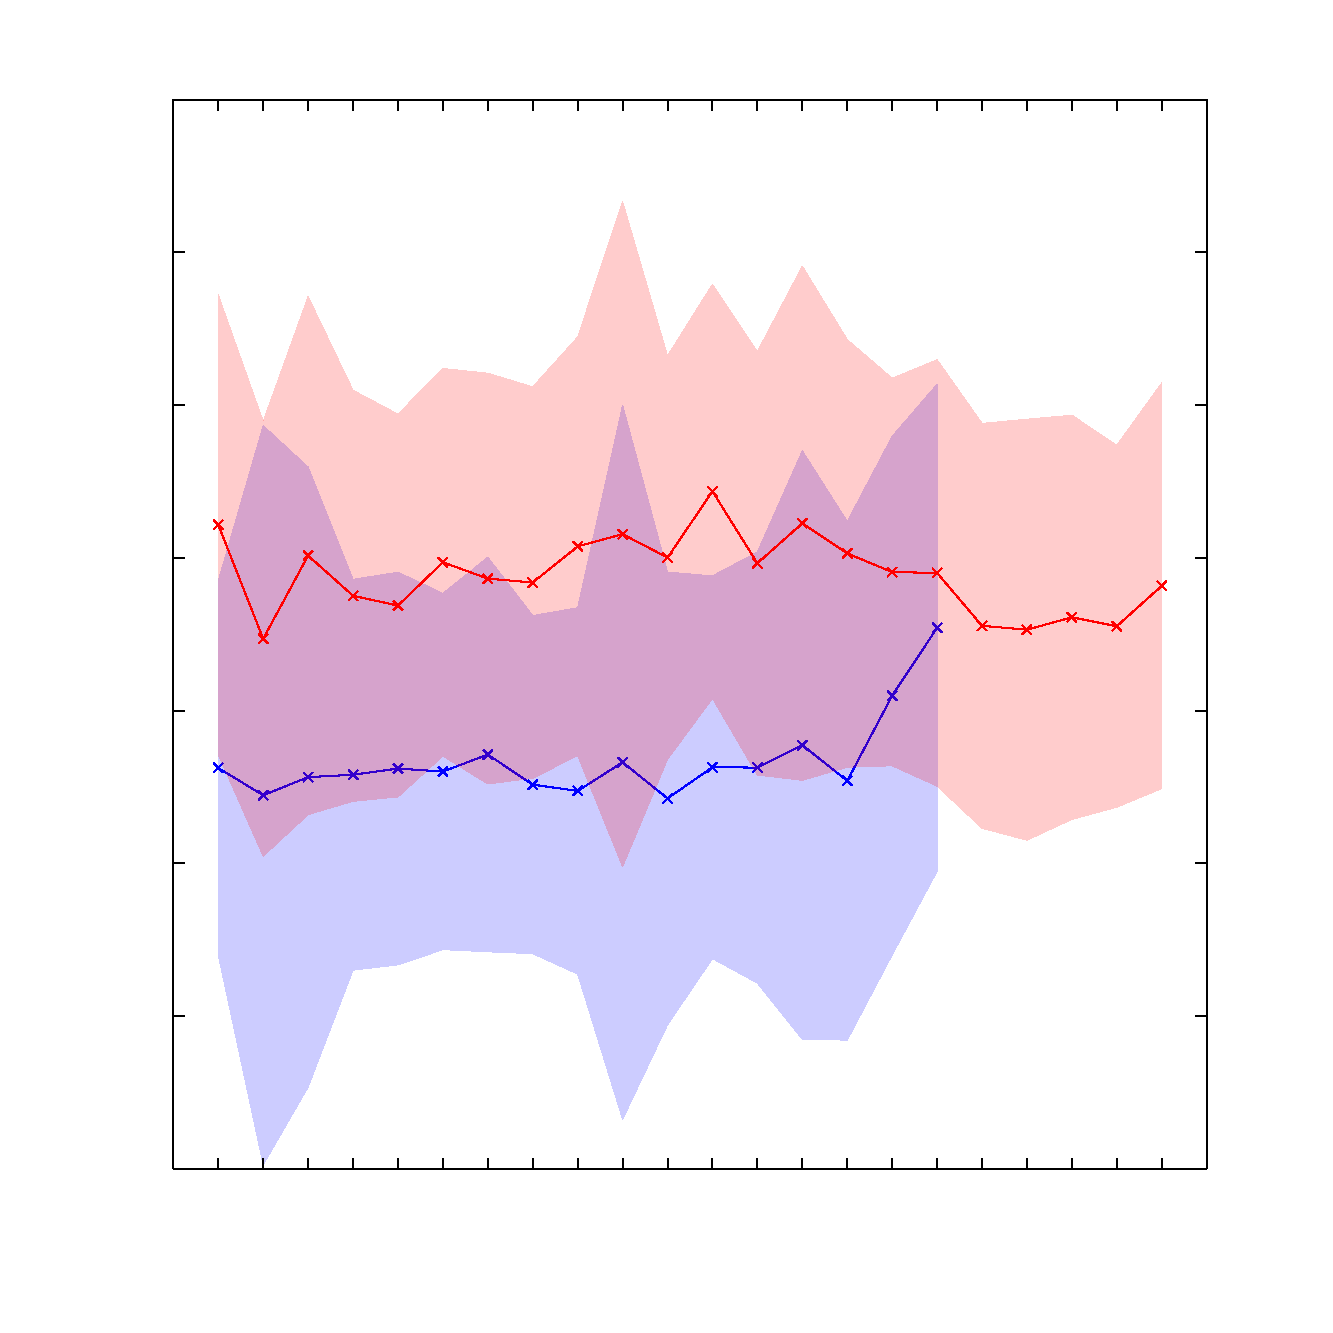
\includegraphics[width=0.47\linewidth]{figs/decoding/rcoef_sess_meanpc_v1_both.pdf}
% }
%     ~~
%     \subfloat[][\label{fig:noise_r_v4_all}\ac{V4}]{
% %         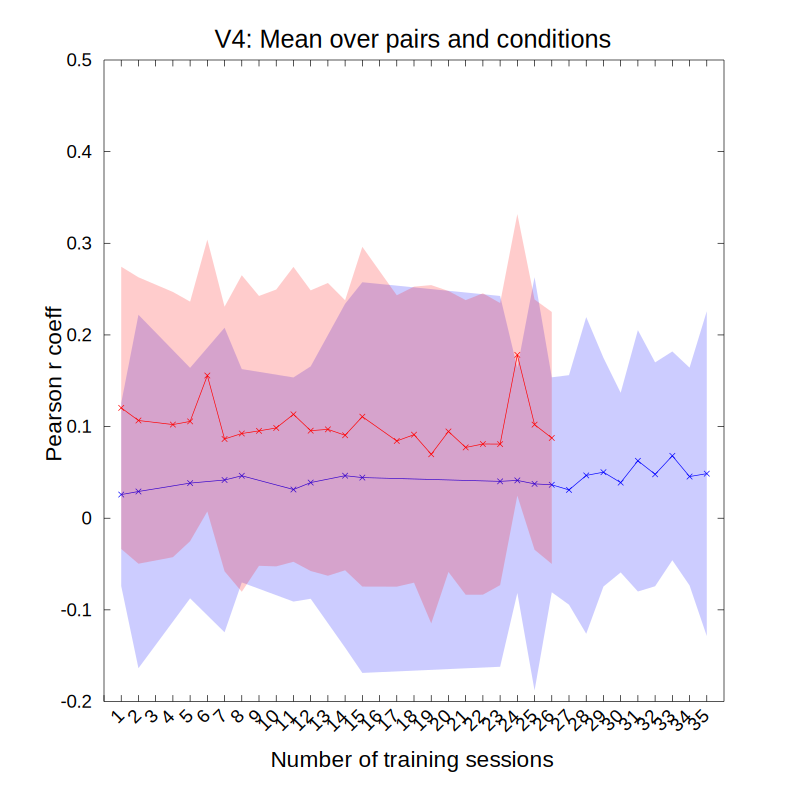
\includegraphics[width=0.47\linewidth]{%
% % ./rcoef_2013-04-09/rcoef_sess_meanpc_2013-04-09/png/rcoef_sess_meanpc_v4_both.png}
%         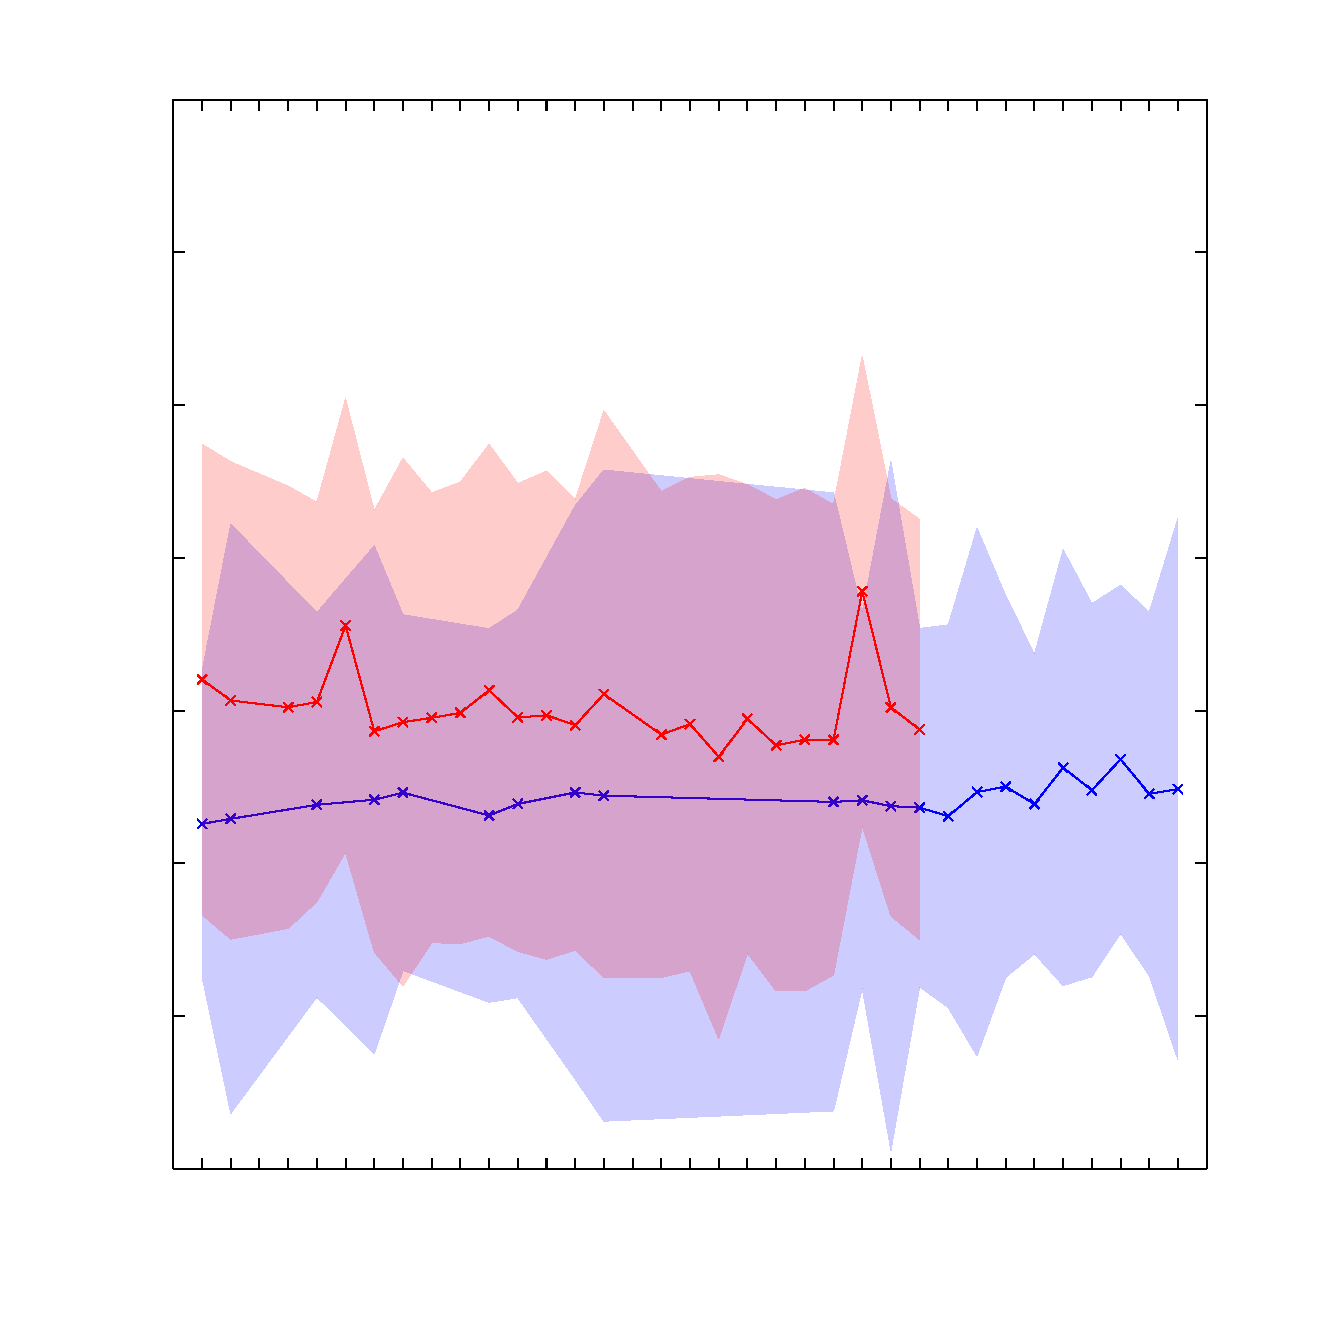
\includegraphics[width=0.47\linewidth]{figs/decoding/rcoef_sess_meanpc_v4_both.pdf}
% }
%     \caption{Change in noise correlations with learning.
% \protect\subref{fig:noise_r_v1_all}:~\ac{V1}.
% \protect\subref{fig:noise_r_v4_all}:~\ac{V4}.
% Blue:~\ac{M1}.
% Red:~\ac{M2}.
% On the x-axis, the number of sessions since the animal began training in the part of the visual field retinotopic to the recording site is shown.
% Line: pearson r coefficient, averaged across the possible pairings between channels for each of the 14 trial conditions.
% Shaded region indicates one standard deviation from mean.
% }
%     \label{fig:noise_r_all}
% \end{figure}
% % \marginnote{In \autoref{fig:noise_r_all} and \autoref{fig:noise_r_hist}, the text is too small due to saving the figure with transparencies in PNG format; if I could get the SVG to load correctly, the text would be sized correctly.}
%
% \autoref{fig:noise_r_hist} is intended to reproduce \citet[Figure 2C]{Gu2011}, with the distribution of $r$ shown across pairs for one pre-training and one post-training session.
% These sessions were chosen from a restricted set of sessions which did not have problems with artificially high correlations from the motion artifact, and selected from this set such that they were as close to the start and end of the training period as possible.
% However, this selection was made before the set of trials was redacted as mentioned in \autoref{sec:dec-meth-noise}, so the sessions selected could possibly be made further apart.
%
% The data presented in \autoref{fig:noise_r_hist} shows that the distribution of noise correlation pairs does not move significantly for \ac{M1} \ac{V1}, which is contrasted by a clear decrease for \ac{M2} \ac{V1}.
% It should be noted though that the distribution for \ac{M2} \ac{V1} begins higher than \ac{M1} and decreases to a similar value as \ac{M1} \ac{V1}.
% For \ac{V4}, there is an increase in mean noise correlation for \ac{M1} and a decrease for \ac{M2}, though as \ac{M2} begins higher than \ac{M1} the two do tend toward to one another.
%
% Cherry-picking is a significant problem here, as there is sizable day-to-day variation in the noise correlation across the pairs.
% Choosing a session where there is more noise correlation than neighbouring sessions at the beginning of training and less at the end of training will give the impression that there is a more significant decrease in noise correlations.
% More effort should be made to counter inadvertently cherry-picking in the session selection, as \autoref{fig:noise_r_j1_pmc} indicates this may be one reason for such a sizable decrease in noise correlation for \ac{M2} \ac{V1}.
%
% \begin{figure}[htbp]
%     \subfloat[][\label{fig:noise_r_b1_hist}]{
%         \centering
% %         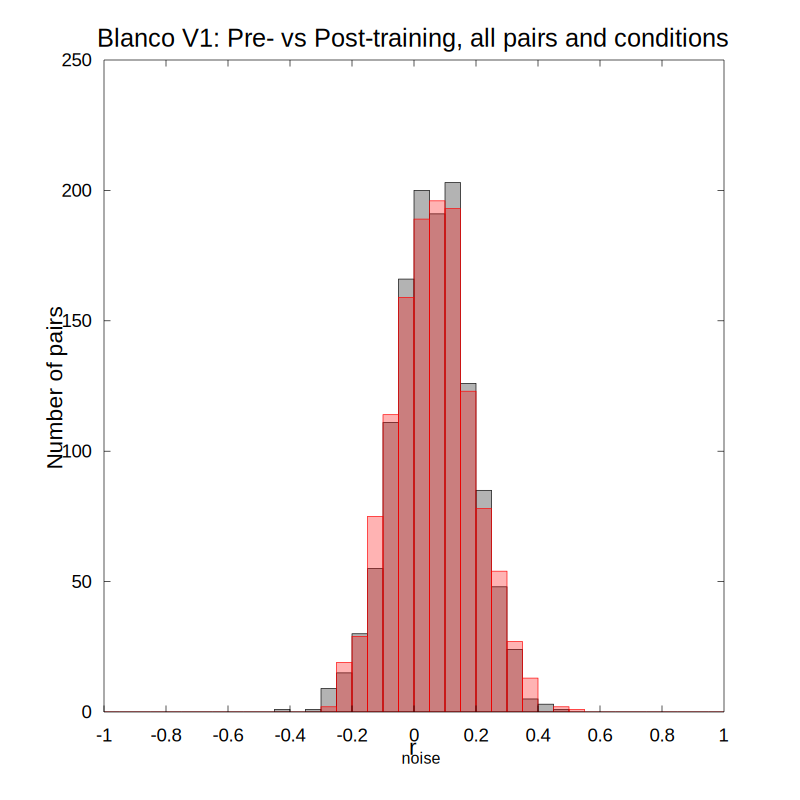
\includegraphics[width=0.47\linewidth]{%
% % ./rcoef_2013-03-25/rcoef_sess_histallover_2013-03-25/png/rcoef_sess_histallover_v1_blanco.png}
%         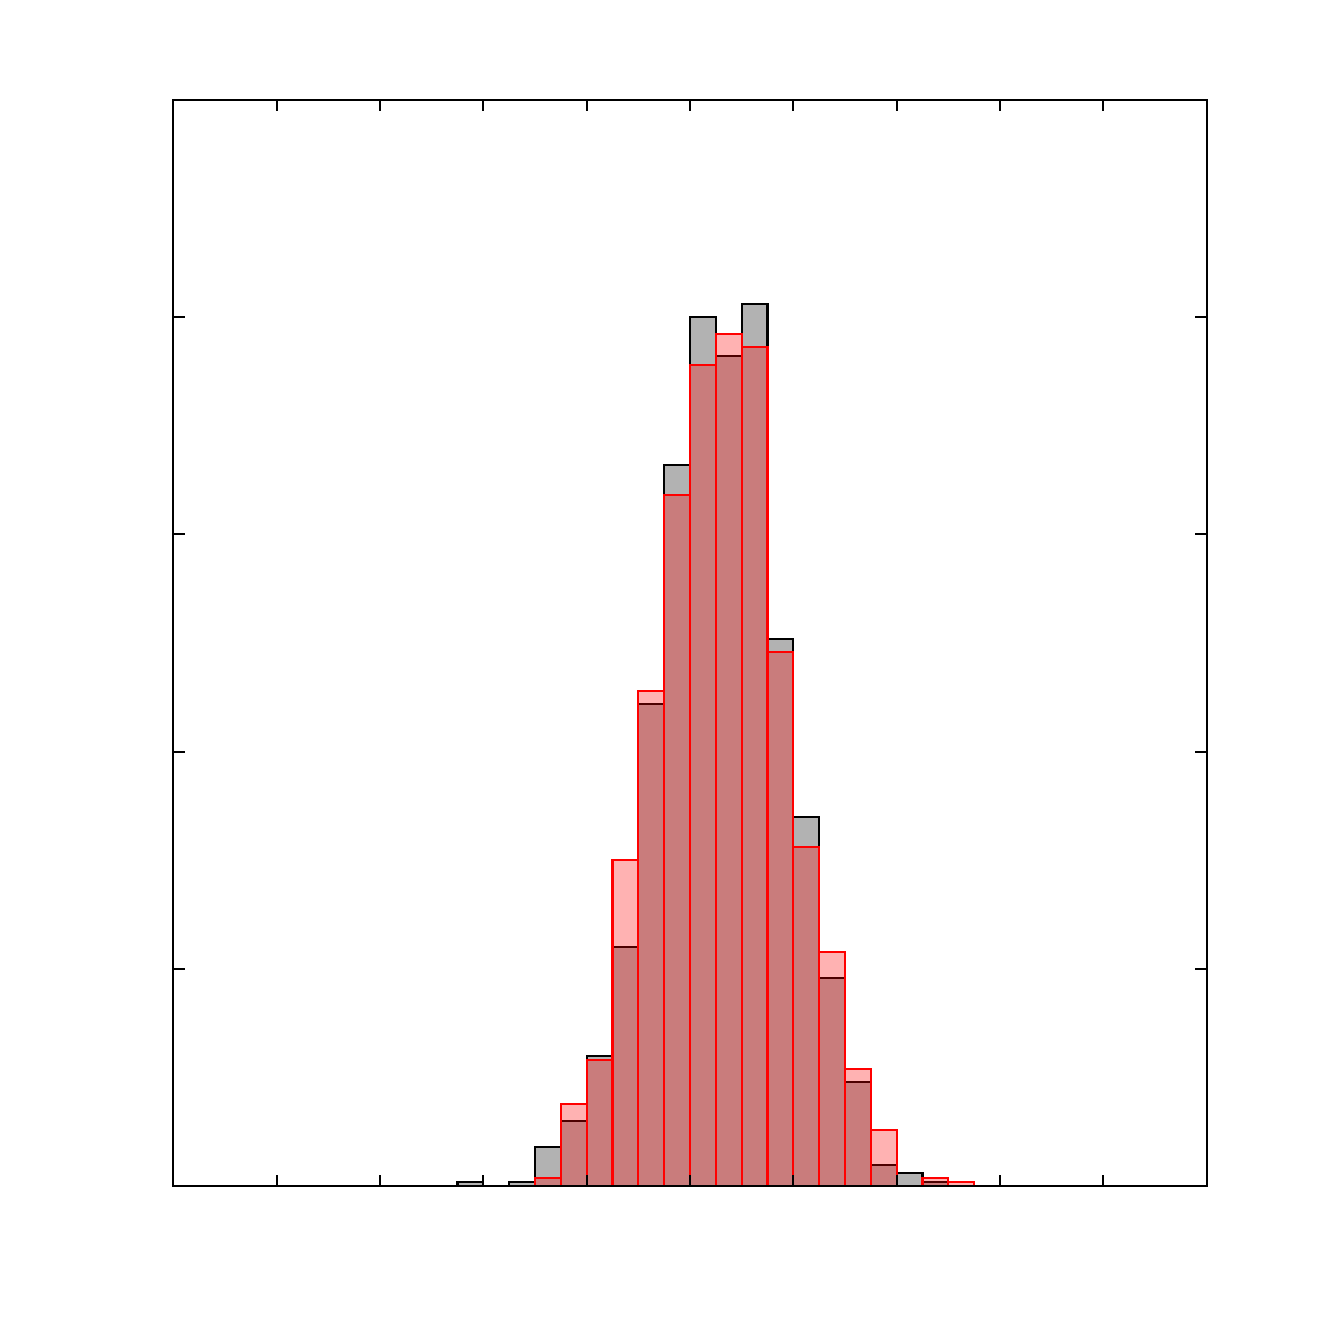
\includegraphics[width=0.47\linewidth]{figs/decoding/rcoef_sess_histallover_v1_blanco.pdf}
%     }
%     ~~
%     \subfloat[][\label{fig:noise_r_j1_hist}]{
%         \centering
% %         \includegraphics[width=0.47\linewidth]{%
% % ./rcoef_2013-03-25/rcoef_sess_histallover_2013-03-25/png/rcoef_sess_histallover_v1_jack.png}
%         \includegraphics[width=0.47\linewidth]{figs/decoding/rcoef_sess_histallover_v1_jack.pdf}
%     }
%     \\
%     \subfloat[][\label{fig:noise_r_b4_hist}]{
%         \centering
% %         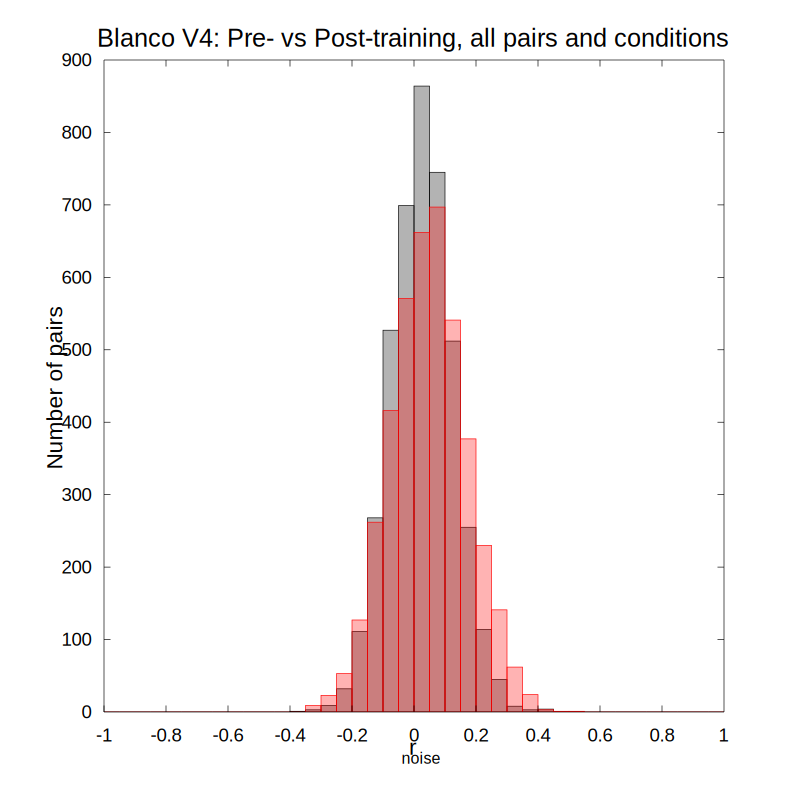
\includegraphics[width=0.47\linewidth]{%
% % ./rcoef_2013-03-25/rcoef_sess_histallover_2013-03-25/png/rcoef_sess_histallover_v4_blanco.png}
%         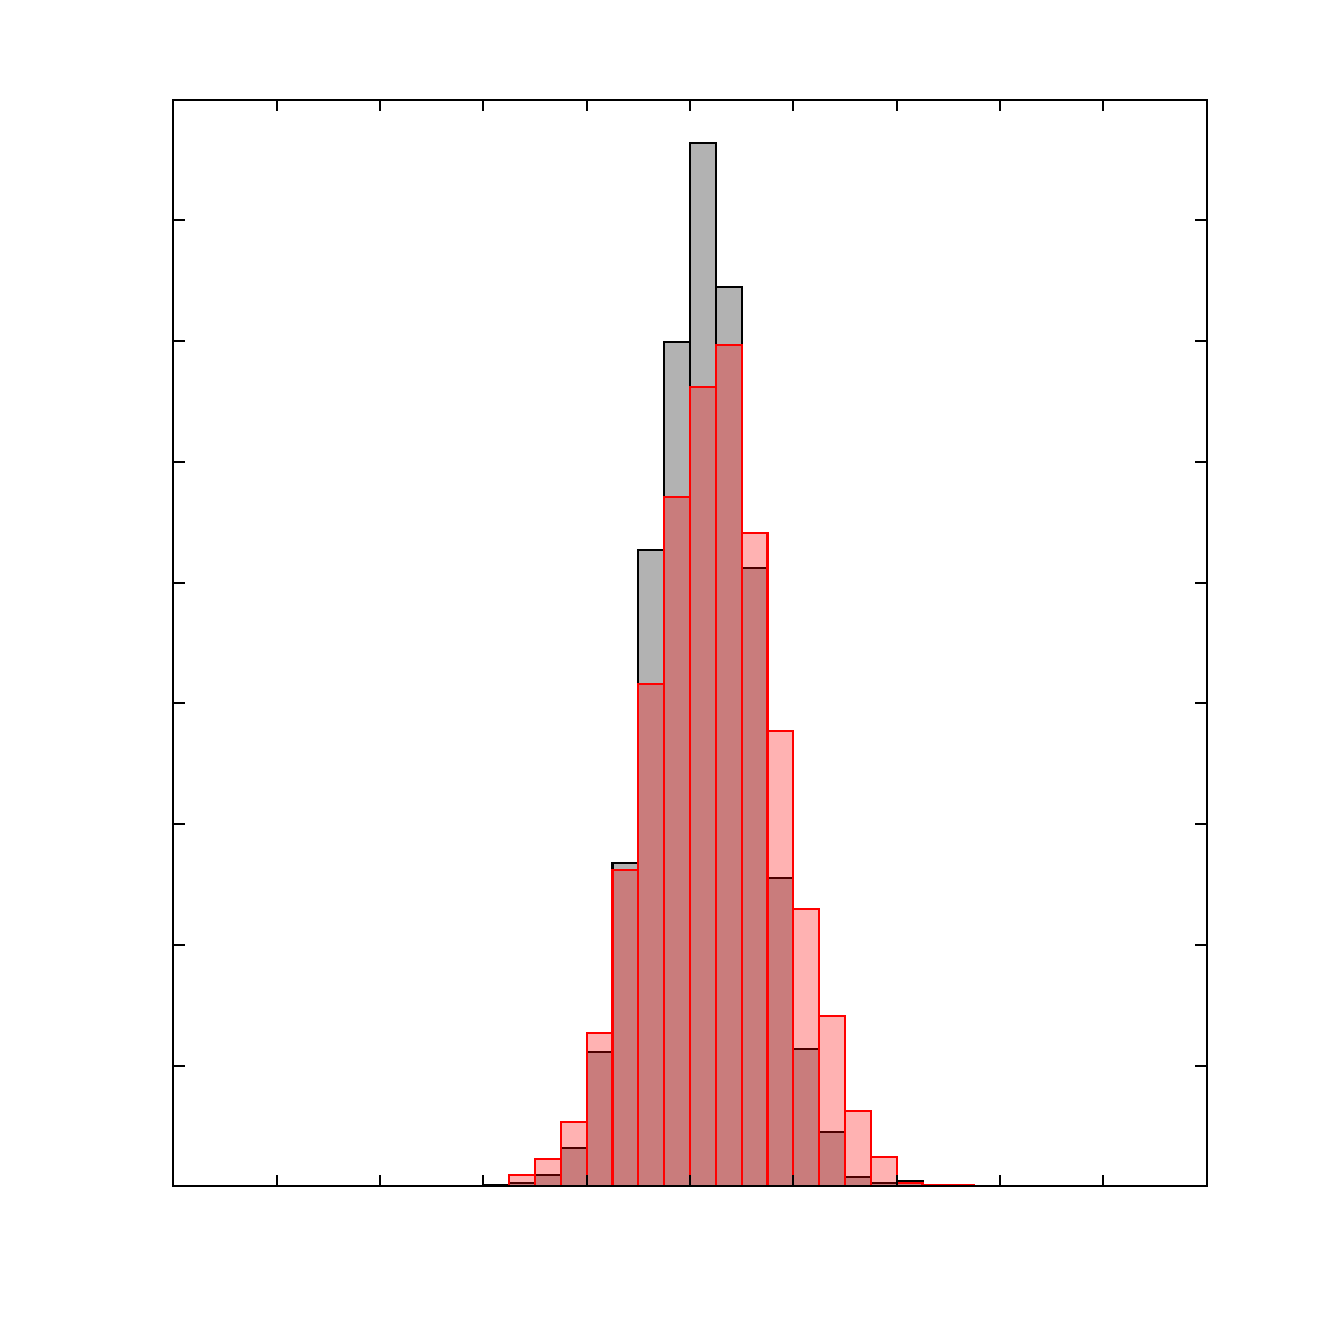
\includegraphics[width=0.47\linewidth]{figs/decoding/rcoef_sess_histallover_v4_blanco.pdf}
%     }
%     ~~
%     \subfloat[][\label{fig:noise_r_j4_hist}]{
%         \centering
% %         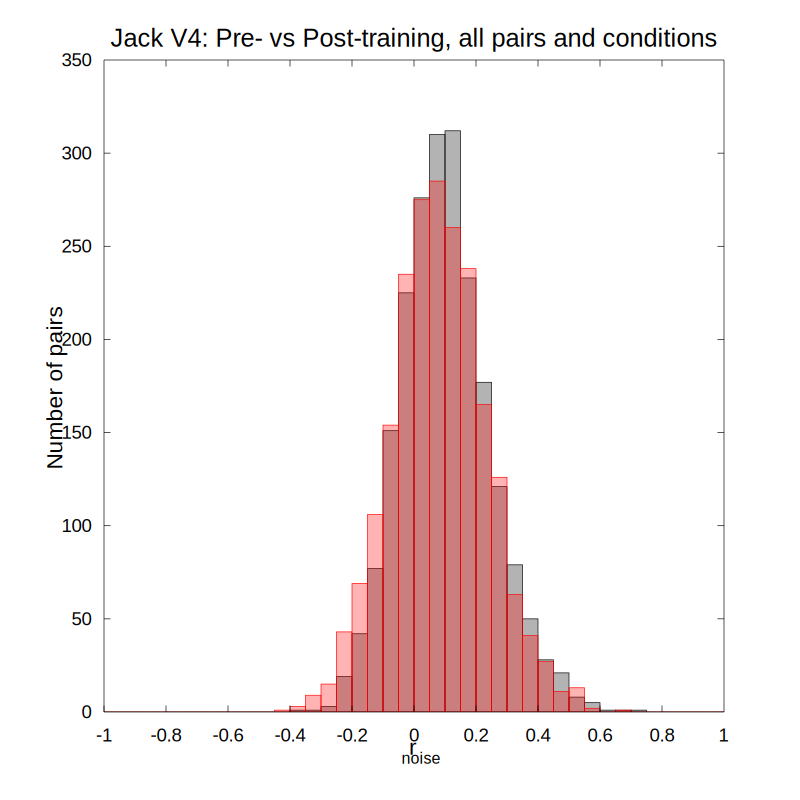
\includegraphics[width=0.47\linewidth]{%
% % ./rcoef_2013-03-25/rcoef_sess_histallover_2013-03-25/png/rcoef_sess_histallover_v4_jack.png}
%         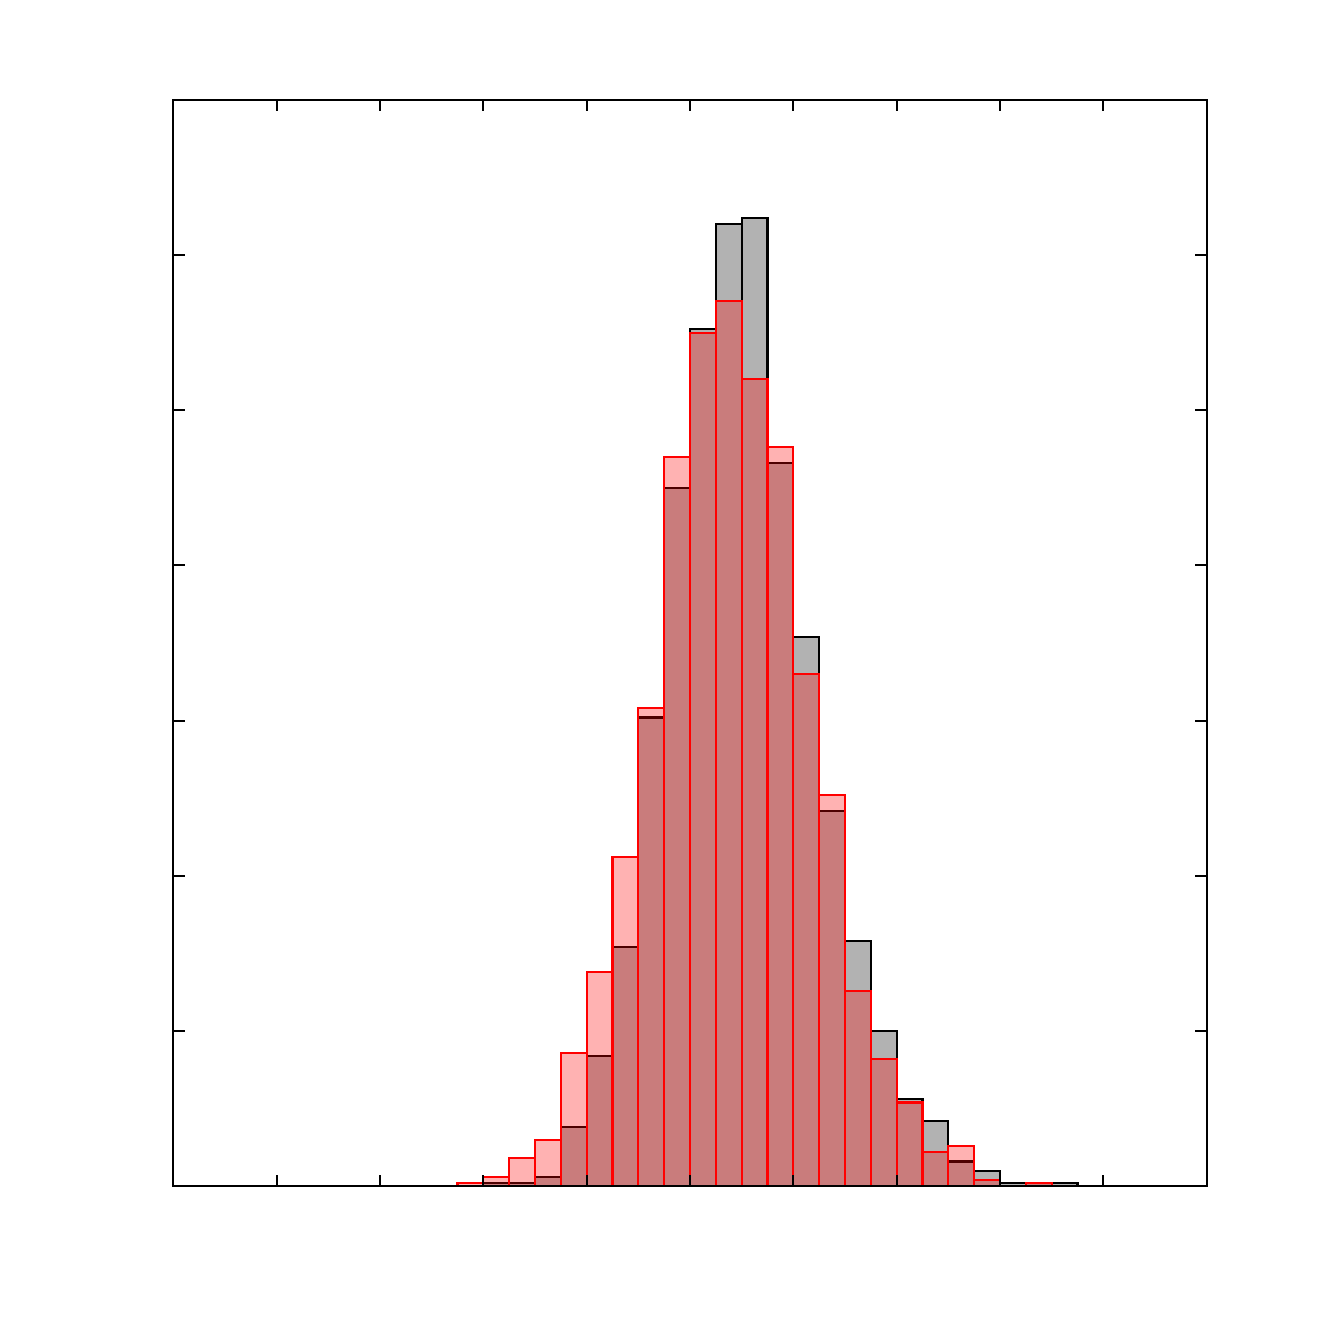
\includegraphics[width=0.47\linewidth]{figs/decoding/rcoef_sess_histallover_v4_jack.pdf}
%     }
%     \caption{Distribution of the noise correlations for the pairings across all conditions.
% Two sessions, one at the beginning of training (black) and one at the end of training (red) are shown for comparitive purposes.
% \protect\subref{fig:noise_r_b1_hist}: \ac{M1} \ac{V1}; sessions 343 and 354.
% \protect\subref{fig:noise_r_j1_hist}: \ac{M2} \ac{V1}; sessions 51 and 71.
% \protect\subref{fig:noise_r_b4_hist}: \ac{M1} \ac{V4}; sessions 307 and 338.
% \protect\subref{fig:noise_r_j4_hist}: \ac{M2} \ac{V4}; sessions 27 and 46.
% }
%     \label{fig:noise_r_hist}
% \end{figure}
%
%
% % \autoref{fig:noise_r_pmc} indicates that noise correlations are correlated for pairs across sessions.
% A pairs of channels which have higher noise correlations in one session are likely to have higher noise correlation in other sessions.
% However, this effect is not present for \ac{M1} \ac{V1}, \autoref{fig:noise_r_b1_pmc}, and could suggest there is less session-to-session consistency for this dataset.
%
% This figure provides an easy way of visually inspecting whether noise correlations are conserved, but does not allow us to quantify this.
%
% \begin{figure}[htbp]
%     \subfloat[][\label{fig:noise_r_b1_pmc}]{
%         \centering
%         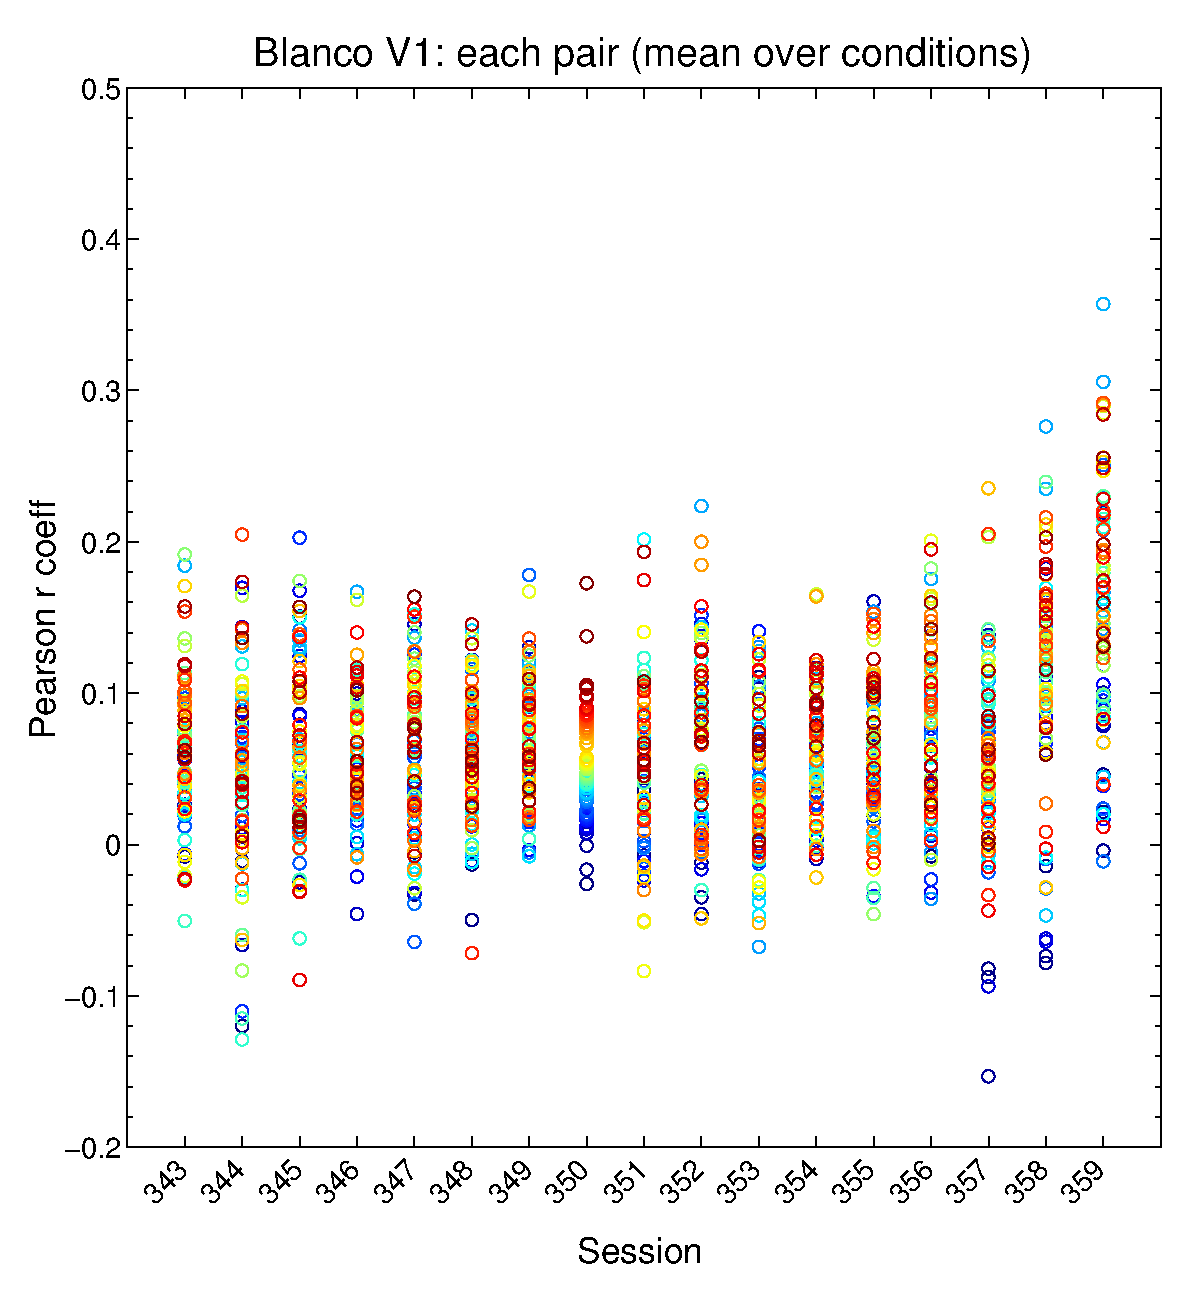
\includegraphics[width=0.47\linewidth]{%
% figs/decoding/rcoef_sess_pairsmeanc_v1_blanco.eps}
%     }
%     ~~
%     \subfloat[][\label{fig:noise_r_j1_pmc}]{
%         \centering
%         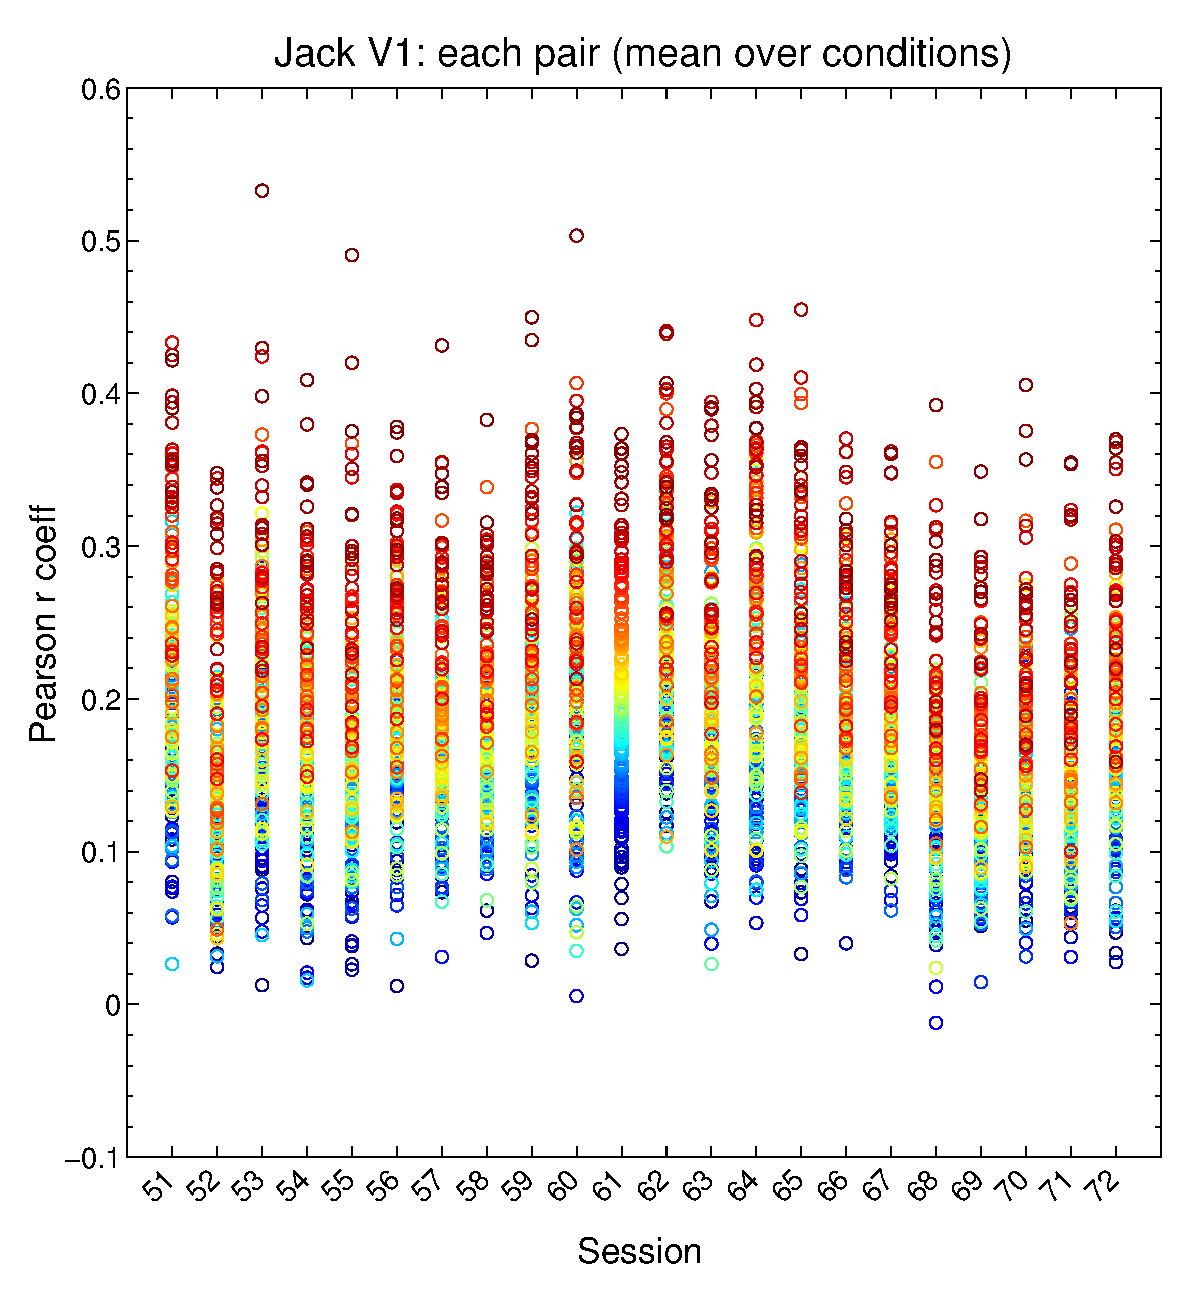
\includegraphics[width=0.47\linewidth]{%
% figs/decoding/rcoef_sess_pairsmeanc_v1_jack.eps}
%     }
%     \\
%     \subfloat[][\label{fig:noise_r_b4_pmc}]{
%         \centering
%         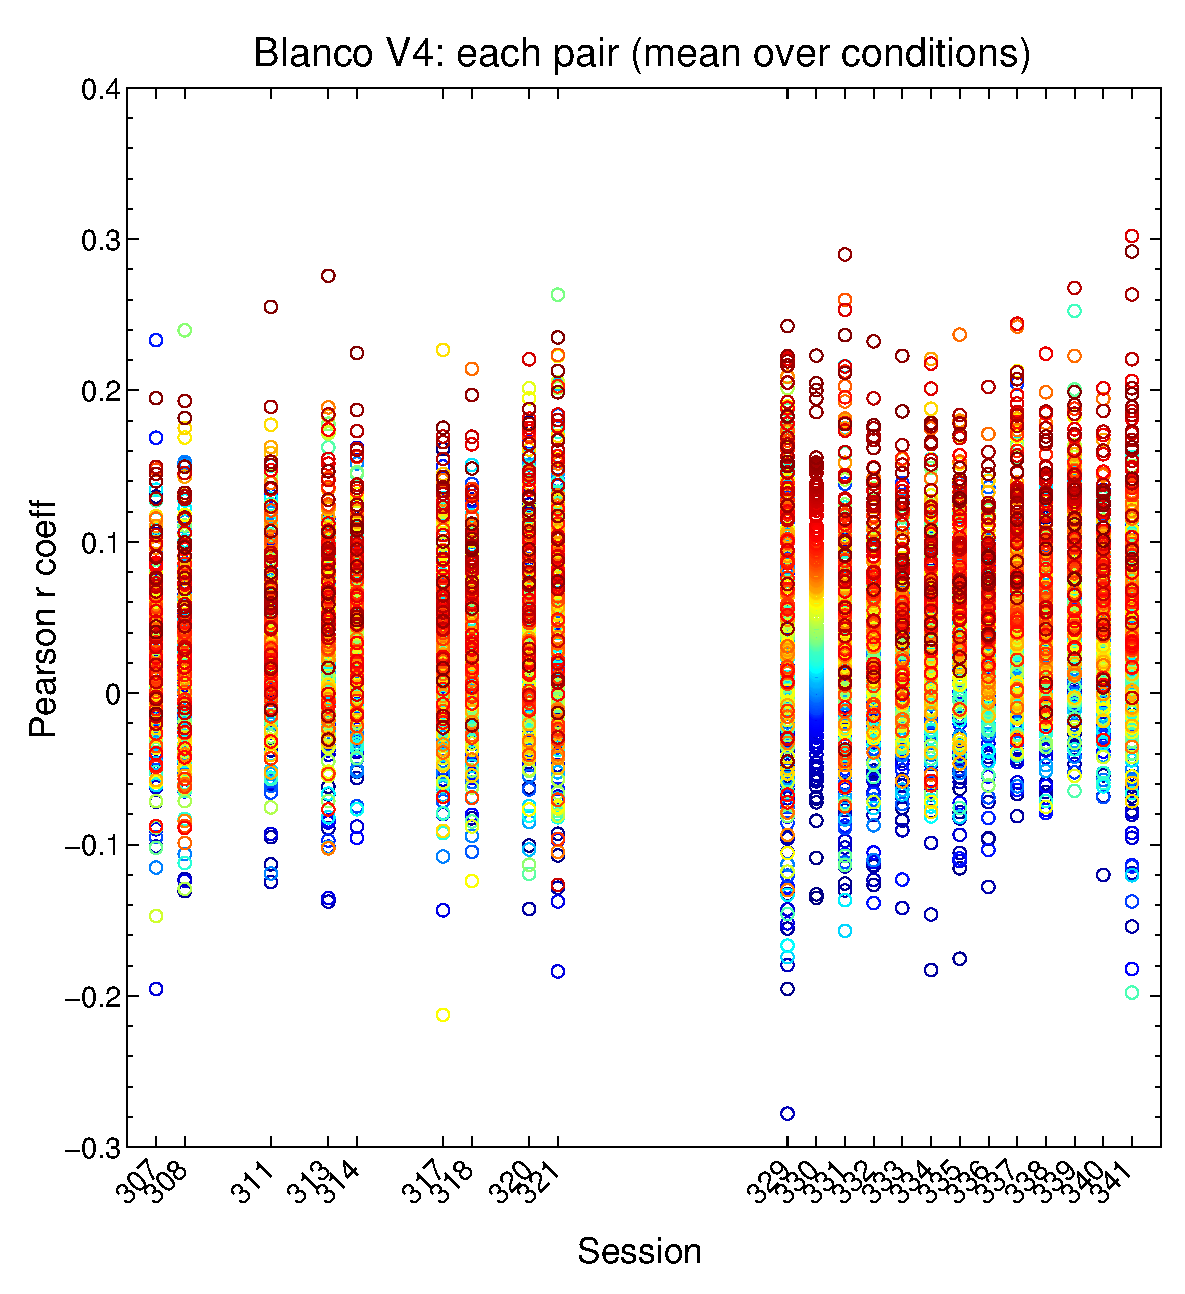
\includegraphics[width=0.47\linewidth]{%
% figs/decoding/rcoef_sess_pairsmeanc_v4_blanco.eps}
%     }
%     ~~
%     \subfloat[][\label{fig:noise_r_j4_pmc}]{
%         \centering
%         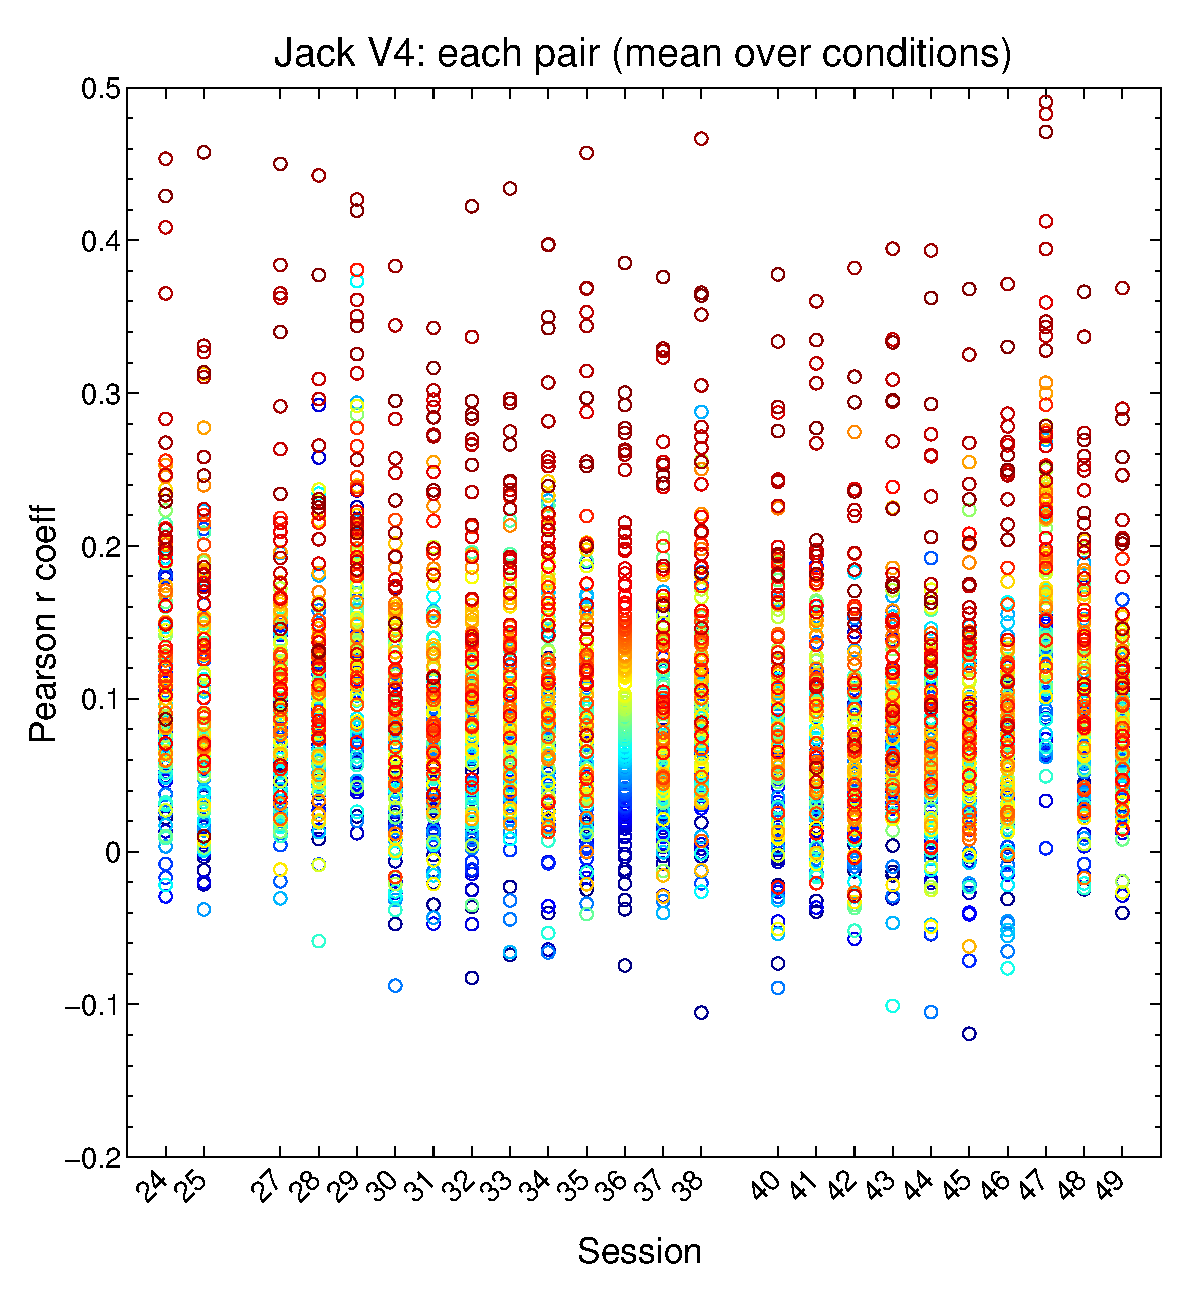
\includegraphics[width=0.47\linewidth]{%
% figs/decoding/rcoef_sess_pairsmeanc_v4_jack.eps}
%     }
%     \caption{Noise correlations for each pair, meaned across the 14 conditions.
% \protect\subref{fig:noise_r_b1_pmc}: \ac{M1} \ac{V1}.
% \protect\subref{fig:noise_r_j1_pmc}: \ac{M2} \ac{V1}.
% \protect\subref{fig:noise_r_b4_pmc}: \ac{M1} \ac{V4}.
% \protect\subref{fig:noise_r_j4_pmc}: \ac{M2} \ac{V4}.
% Colour is assigned by sorting the pairs into ascending order for one of the sessions near the middle of the training period.
% The degree of session-to-session correlation of the noise correlation can hence be inferred by visual inspection.
% }
%     \label{fig:noise_r_pmc}
% \end{figure}
%
%
%==============================================================================
\section{Sensitivity analysis}
%------------------------------------------------------------------------------

One simple method of comparing how the encoding of stimuli changes over time is to use the amount the sensitivity index, $d'$.
This gives a measure of how separable the signal and the noise are, by comparing the difference in their means with the overall standard deviation.
% For a classifier, this is defined as the difference between the hit rate and the false alarm rate,
% \begin{equation}
% d' = P(A | A) - P(A | \bar{A})
% ,\end{equation}

For Gaussian distributed data, the sensitivity index is defined as
\begin{equation}
d' = \frac{\mu_\text{stim} - \mu_\text{noise}}{\sigma_\text{joint}}
,\end{equation}
where the joint standard deviation is the over for the two distributions,
\begin{equation}
% \sigma_\text{joint} = \sqrt
%     \frac{ (n_\text{stim}-1) \, \sigma_\text{stim}^2 + (n_\text{noise}-1) \, \sigma_\text{noise}^2 }
%     { n_\text{stim} + n_\text{noise} - 2}
\sigma_\text{joint} = \sqrt \frac{\sigma_\text{stim}^2 + \sigma_\text{noise}^2}{2}
.\end{equation}
For our analysis, the noise is the spiking activity during periods of spontaneous activity.
With the sample stimulus and 14 test stimuli with differing contrast levels, we have 15 possible signals to choose from for each dataset.
Since it has the most presentations and lies in the middle of the range of the contrasts, we will just consider $d'$ with respect to the response signal when presenting the sample stimulus.

The number of spikes over a finite duration, which cannot be negative, is Poisson distributed instead of Gaussian distributed.
However, the two distributions do converge for large $n$, and so we disregard this and use the Gaussian form of the definition of $d'$.

%------------------------------------------------------------------------------
\subsection{Methods}

To compute $d'$, we considered the signal and noise to be the number of spikes occurring during a \SI{150}{\milli\second} period of activity.
For spontaneous (noise) activity, this was the \SI{150}{\milli\second} immediately preceding the sample stimulus onset.
For signal activity, this was the \SI{150}{\milli\second} either \SI{30}{\milli\second} (\ac{V1}) or \SI{60}{\milli\second} (\ac{V4}).
This delay was used to approximately account for the minimal possible response latency in \ac{V1} and \ac{V4}.

The violin plots showing the distribution over channels of $d'$ before and after training were created by taking a Gaussian kernel density with a bandwidth of 0.15.
This bandwidth was determined using the rule of thumb bandwidth estimator,
\begin{equation}
w = \hat{\sigma} \left( \frac{4}{3 n} \right) ^ \frac{1}{5}
,\end{equation}
for each animal and area on the distribution before and after training, and using the minimum of these 8 values.
This ensures sufficient detail about the distribution is captured for each distribution, and all are comparable with each other.

To investigate whether $d'$ changed significantly during the course of our experiments, we compared the average $d'$ during the first 3 and final 3 experimental sessions (\zonename{A} and \zonename{B}).
A paired $t$-test (two-tailed) was used to study whether the $d'$ consistently increased or decreased for the channels.

%------------------------------------------------------------------------------
\subsection{Results}

\subsubsection{V1}

For \ac{V1}, we found the $d'$ decreased with training (see \autoref{fig:dprime_v1}).
A similar result was observed for each subject.
The average change in was $\Delta d' = -0.324$ ($p=0.02$, paired $t$-test) for \ac{M1} and $\Delta d' = -0.417$ ($p < 3 \times 10 ^{-10}$, paired $t$-test) for \ac{M2}.
 
\begin{figure}[htbp]
    \centering
    \hspace*{\fill}
    \subfloat[\ac{M1} \ac{V1}\label{fig:dprime_v1_blanco}]{
        \centering
        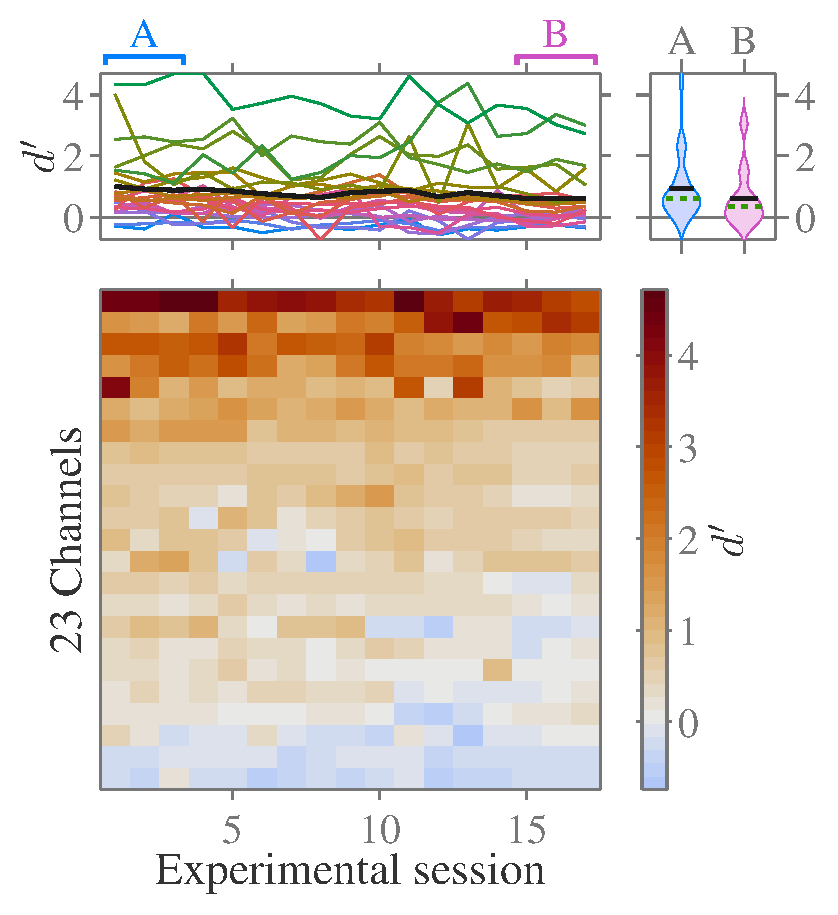
\includegraphics[scale=.45]{%
figs/dprime/dprime_sample_hm_hotcold_blanco_v1_1_rmon2_rmvet2.eps}
    }
    \hspace*{\fill}\hspace{.2cm}\hspace*{\fill}
    \subfloat[\ac{M2} \ac{V1}\label{fig:dprime_v1_jack}]{
        \centering
        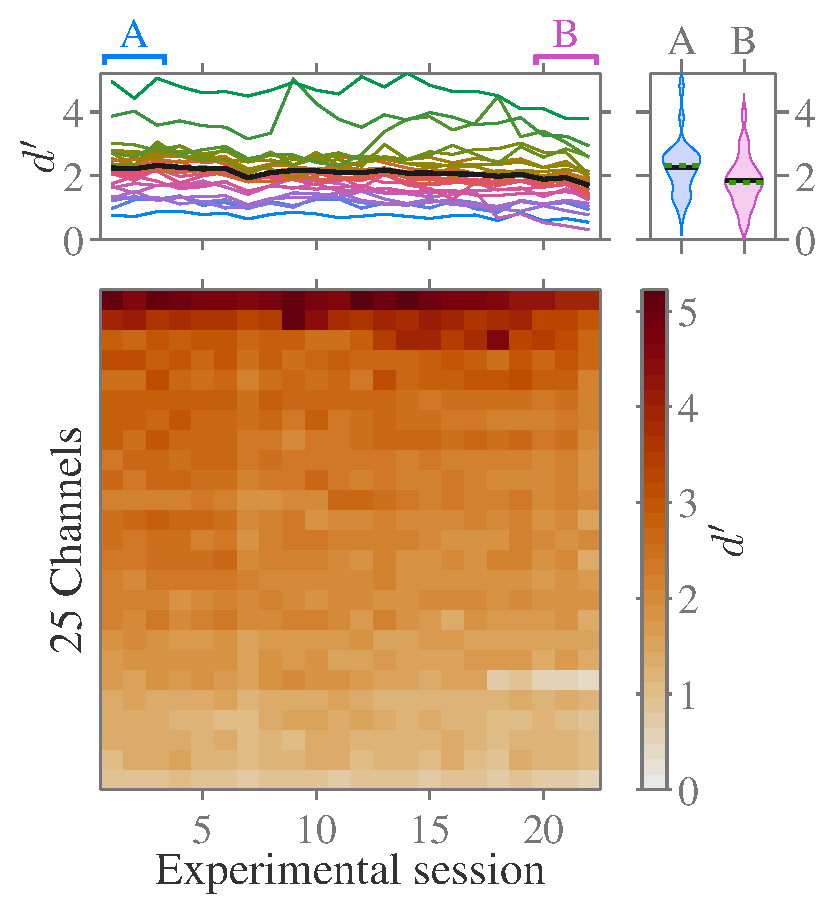
\includegraphics[scale=.45]{%
figs/dprime/dprime_sample_hm_hotcold_jack_v1_1_rmon2_rmvet2.eps}
    }
    \hspace*{\fill}
    \caption{Change in $d'$ over training sessions for \ac{V1} recordings.
\protect\subref{fig:dprime_v1_blanco}: $d'$ for \ac{M1}, shown for each recording channel, with channels ordered according to average $d'$ over all sessions.
Above, traces of $d'$ for each channel (colours), and average over channels (black).
Below, heatmap showing $d'$ for each channel.
Right top, violin plots showing distribution over channels of the average $d'$ in the first three sessions (\zonename{A}) and last three sessions (\zonename{B}), with mean (solid black line) and median (dashed green line) over channels indicated.
The violin plot shows a Gaussian kernel density using a bandwidth determined automatically as described in \autoref{sec:info-methods}.
\protect\subref{fig:dprime_v1_jack}: Same as \protect\subref{fig:dprime_v1_blanco}, but for \ac{M2}.
}
    \label{fig:dprime_v1}
\end{figure}


\subsubsection{V4}

This is in contrast with our findings for \ac{V4}.
For \ac{M1}, some channels marginally increased and others marginally decreased their $d'$ with training (\autoref{fig:dprime_v4_blanco}).
Overall, there was a small increase in average $d'$, with $\Delta d' = +0.053$, which was not a statistically significant change ($p=0.46$).

With \ac{M2}, many channels began training either indifferent to the stimulus, $d'=0$, or suppressed by it, $d'<0$ (\autoref{fig:dprime_v4_jack}).
Starting from this lower position, there was a significant increase of $\Delta d' = +0.491$ ($p < 7 \times 10 ^{-8}$).
However the final $d'$ for almost all channels recorded for \ac{M2} was still lower than the average $d'$ for \ac{M1}.

\begin{figure}[htbp]
    \centering
    \hspace*{\fill}
    \subfloat[\ac{M1} \ac{V4}\label{fig:dprime_v4_blanco}]{
        \centering
        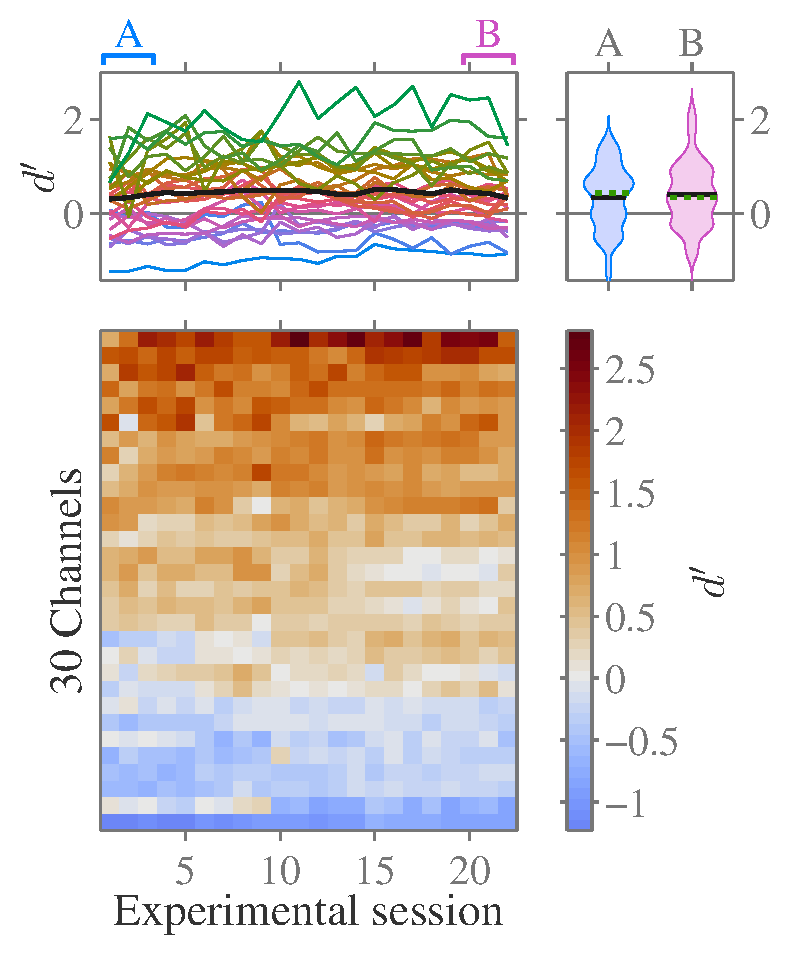
\includegraphics[scale=.45]{%
figs/dprime/dprime_sample_hm_hotcold_blanco_v4_1_rmon2_rmvet2.eps}
    }
    \hspace*{\fill}\hspace{.2cm}\hspace*{\fill}
    \subfloat[\ac{M2} \ac{V4}\label{fig:dprime_v4_jack}]{
        \centering
        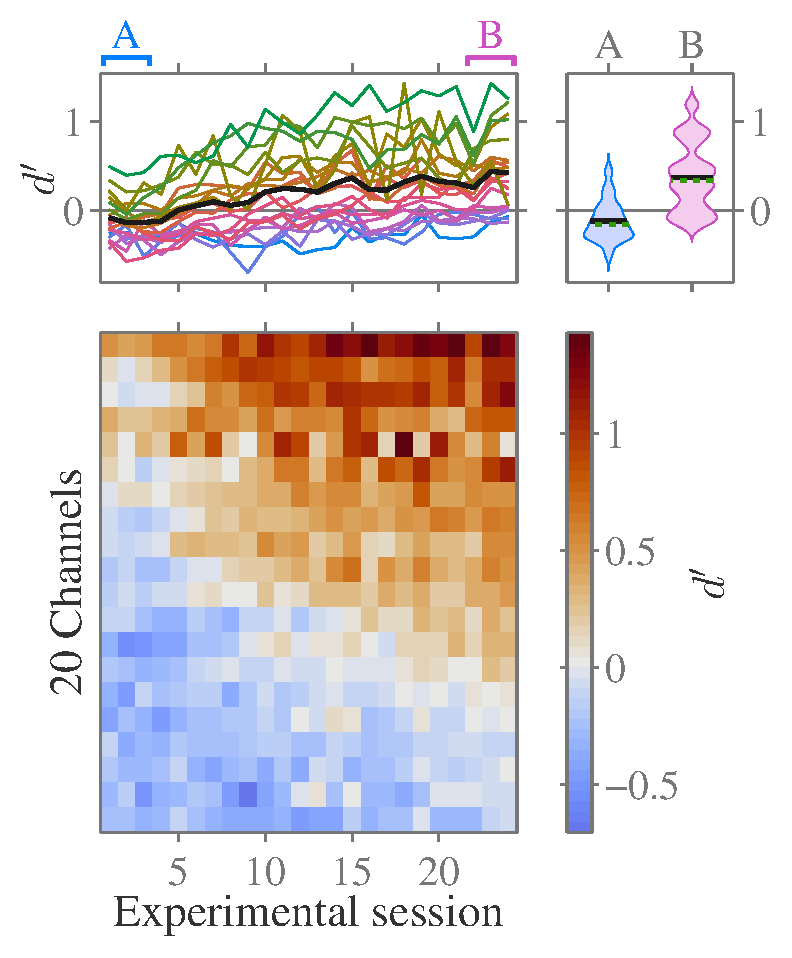
\includegraphics[scale=.45]{%
figs/dprime/dprime_sample_hm_hotcold_jack_v4_1_rmon2_rmvet2.eps}
    }
    \hspace*{\fill}
    \caption{Same as \autoref{fig:dprime_v1}, but for $d'$ during \ac{V4} recordings.
\protect\subref{fig:dprime_v4_blanco}: \ac{M1}.
\protect\subref{fig:dprime_v4_jack}: \ac{M2}.
}
    \label{fig:dprime_v4}
\end{figure}


\subsection{Discussion}
\label{sec:pl_dprime_discuss}

By analysing the sensitivity index, $d'$, we can see whether channels become more or less responsive to our stimulus class over time.
Since \ac{V1} is an early step in the visual processing hierarchy, its neurons respond strongly to simple stimuli such as the sinusoidal gratings we present.
Consequently, neurons have large responses to our stimuli even from the first session of the experimental training.
Over time, we found a decrease in sensitivity in \ac{V1} for both subjects.
We suspect this decrease in sensitivity of the neural response in \ac{V1} to the sample stimulus is due to unpreventable deterioration in the recording quality of the implanted chronic electrodes over time.
Overtime, the noise increases and the signal-to-noise ratio falls, which leads to a reduction in the distinguishability of the two activity distributions.

On the other hand, \ac{V4} is higher up the visual hierarchy and in general responds to more a complex stimulus class.
For \ac{M1}, many of the neurons we recorded from were responsive to the primitive Gabor stimulus from the beginning of training.
But for \ac{M2}, this was not the case --- on the contrary, many neurons were suppress by the Gabor stimulus.
With training, neurons recorded in \ac{M1} did not notably change their sensitivity to the sample stimulus, whereas $d'$ did increase for \ac{M2}.

We make particular note of the fact that the $d'$ in \ac{V4} increased for \ac{M2} from mostly negative initially values.
In principle, a decrease in activity in response to a stimulus can provide as much information about the presence of the stimulus as increase in activity.
However, it is difficult for neurons to increase their spontaneous activity due to the constraining effects of homeostasis, and it would be energetically inefficient for them to do so.
Therefore, since the firing rate of a neuron cannot fall below $0$ there is a smaller limit to the amount by which firing rates can differ if the information about the stimulus is conveyed by a reduction in activity compared to the background rate.
To provided more sensitivity for the response to our experimental stimuli, it thus makes sense for neurons which are suppressed by the stimulus class to increase their responses such that they are enhanced by its presence.
In practice, the de-suppression of the responses may arise not from the need of many individual neurons to encode the stimulus, but from a small number increasing the magnitude of their responses and then the connected neurons (which are positively correlated) increase their responses also.

From these results, we hypothesise that the sensitivity of the response to the experimental stimuli increases for the local network retinotopic to the stimulus location if it is too low for the network overall.
If the neurons are sufficiently sensitive to the stimulus to begin with (if $d'$ is high enough) then the sensitivity remains the same and does not increase with training.
Of course, the recorded sensitivity may decrease due to the decline in the recording quality.

With this measure, we can determine which channels contain neurons which change their relative responsiveness to the stimulus class, but we do not know how the distribution of responses change across the 14 different stimuli.
It is certainly plausible for neurons which begin their training already responsive to the stimuli to change their distribution of activity with respect to the contrast of the stimulus to provide more pertinent information for the experimental task.
For instance, this would be achieved if the absolute activity in response to the sample stimulus remains the same but the rate of change of activity with respect to the contrast of the stimulus increases.


%==============================================================================
\FloatBarrier
\section{Information in individual channels}
%------------------------------------------------------------------------------

We now apply the principles of Shannon information, as described in \autoref{sec:bgit}, to the perceptual learning data.
We are interested in how easy it is to determine which contrast the stimulus was presented with by observing the neural activity in response to the stimulus.
Since the subject's performance increases with training, we expect to find the amount of information encoded in the neural activity to increase with training.

To make its decision, the subject has access to all the neurons we have recorded and all the neurons in the brain from which we have not recorded.
Consequently, it would for the best idea of how much information the brain has access to, we would evaluate how much information is contained in the vector of neuronal responses for every recording channel.
However, this is problematic.
As the number of data streams combined into the response vector increases, the number of possible unique response vectors increases exponentially.
However, the number of trials recorded over is held fixed, and the number of possible response vectors must be constrained to prevent the estimated amount of information diverging to infinity (see \autoref{sec:bgit}).

Therefore, in this section we consider the information about the contrast of the stimulus encoded in the firing rate detected from only a single channel at once.
Because the spikes detected from each channel have been left unsorted and not resolved into clusters corresponding to individual neurons, this will be a multi-unit analysis, but only in the sense of neighbouring neurons being detected by the same electrode contact.


%------------------------------------------------------------------------------
\subsection{Methods}
\label{sec:info-methods}

The mutual information between the spiking activity during the presentation of the test stimulus and the identity of that stimulus was computed using the \textit{Information Breakdown Toolbox} for MATLAB \citep{Magri2009}.
Bias correction was performed using the \ac{PT} method (see \autoref{sec:bgit}) unless indicated otherwise.

The distribution of information over channels is shown using violin plots indicating the Gaussian kernel density with an automatically selected bandwidth.
We state the rule-of-thumb Gaussian basis bandwidth estimator as
\begin{equation}
h = \left( \frac{4}{3n} \right) ^ \frac{1}{5} \, \hat{\sigma}
,\label{eq:estimate-bw}\end{equation}
where $n$ is the number of samples and $\hat{\sigma}$ is the estimated standard deviation over the distribution.
We used \autoref{eq:estimate-bw} to find a suitable kernel basis bandwidth for the distribution over channels of information at the start (\zonename{A}) and end (\zonename{B}) of training.
For the plots, we selected the minimum of $\nicefrac{h_A}{2}$ and $\nicefrac{h_B}{2}$, to ensure sufficient detail was captured and the two distributions were comparable.

To test the significance of changes in information over time, we used a paired Student's $t$-test to compare the difference in information values in $\SET{\zonename{A}}$ and $\SET{\zonename{B}}$ against the null-hypothesis of no change between points \zonename{A} and \zonename{B}.
Although the distribution of information values is evidently non-Gaussian (it is bounded below at \SI{0}{bits}), the distribution in differences in information is close to Gaussian.
We could instead have used the Mann--Whitney $U$ test to compare the two distributions $\SET{\zonename{A}}$ and $\SET{\zonename{B}}$.
This test does not assume the two distributions are Gaussian, but makes the additional assumption that all samples are independent.
Since we record from the same set of channels for both $\SET{\zonename{A}}$ and $\SET{\zonename{B}}$, we are violating the independence assumption, and so the paired Student's $t$-test is a more appropriate choice.


%------------------------------------------------------------------------------
\subsection{Initial analysis}

First, we will consider the amount of information about the stimulus contained in a simple firing rate encoding.
For each test stimulus presentation, our response is the total number of spikes which were detected from a single channel during the first \SI{527}{\milli\second} of the stimulus presentation.%
\footnote{This duration is chosen because there is slight variation in the stimulus presentation time, and \SI{527}{\milli\second} is the shortest presentation duration.}

For each recording channel, we computed how much information was contained in this overall firing response about the identity of which stimulus had been presented.
The results of this initial analysis are shown in \autoref{fig:info_sess_1x527}.
We found that information in the overall firing rate of \ac{V1} channels increased with training for \ac{M2} (\SI{+0.069\pm0.017}{bits} or \SI{+16\pm5}{\percent} relative change, $p=0.0004$) but not for \ac{M1} (\SI{-0.051\pm0.029}{bits} or \SI{-34\pm19}{\percent}, $p=0.09$).
For \ac{V4}, there was an increase in information for both subjects however this increase was significant for \ac{M2} (\SI{+0.056\pm0.013}{bits} or \SI{+87\pm21}{\percent}, $p=0.0005$) but not \ac{M1} (\SI{+0.028\pm0.020}{bits} or \SI{+22\pm16}{\percent}, $p=0.17$).


\begin{figure}[htbp]%
    \centering
    \hspace*{\fill}
    \subfloat[][\ac{M1} \ac{V1}.\label{fig:info_sess_1x527_v1_blanco}]{%
        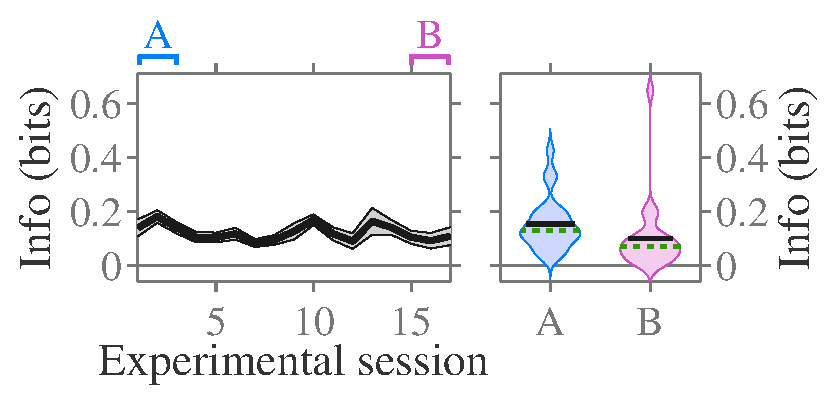
\includegraphics[scale=.45]{%
figs/info2/I_sessionwise_blanco_v1_chmean23_s343-359_oc0_G_1bins_of_527ms_dr_pt_rmvet2_rmvms2_imscn_clhot.eps}}
    \hspace*{\fill}\hspace{.2cm}\hspace*{\fill}
    \subfloat[][\ac{M2} \ac{V1}.\label{fig:info_sess_1x527_v1_jack}]{%
        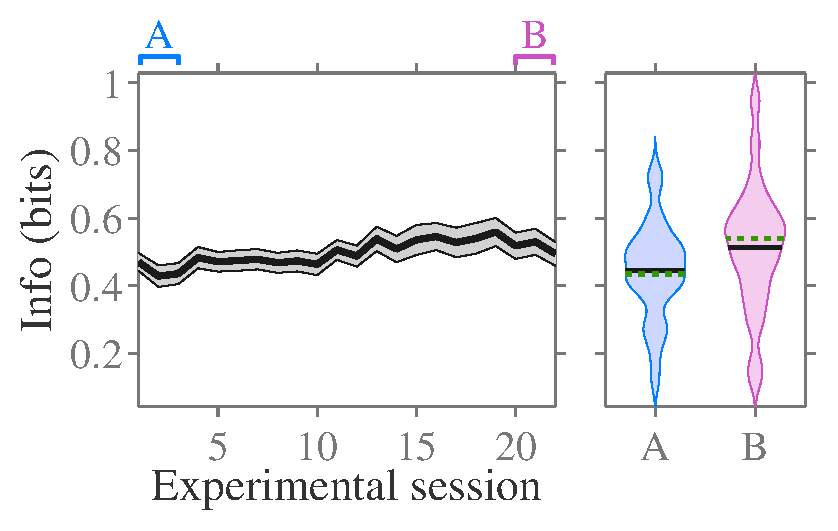
\includegraphics[scale=.45]{%
figs/info2/I_sessionwise_jack_v1_chmean25_s51-72_oc0_G_1bins_of_527ms_dr_pt_rmvet2_rmvms2_imscn_clhot.eps}}
    \hspace*{\fill}
    \\
    \hspace*{\fill}
    \subfloat[][\ac{M1} \ac{V4}.\label{fig:info_sess_1x527_v4_blanco}]{%
        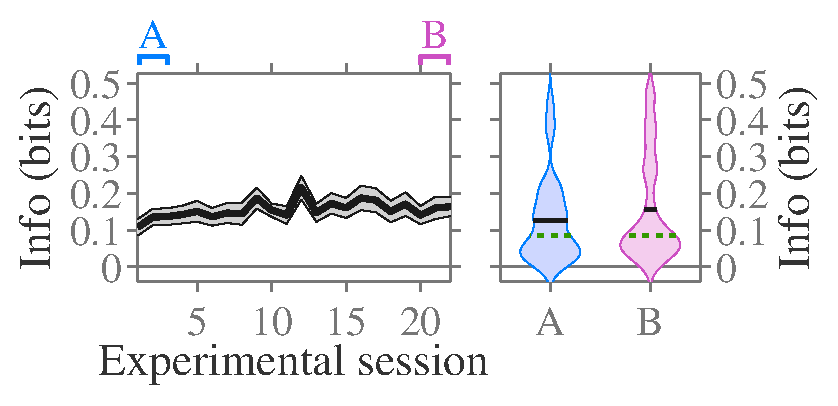
\includegraphics[scale=.45]{%
figs/info2/I_sessionwise_blanco_v4_chmean30_s307,308,311,313,314,317,318,320,321,329-341_oc0_G_1bins_of_527ms_dr_pt_rmvet2_rmvms2_imscn_clhot.eps}}
    \hspace*{\fill}\hspace{.2cm}\hspace*{\fill}
    \subfloat[][\ac{M2} \ac{V4}.\label{fig:info_sess_1x527_v4_jack}]{%
        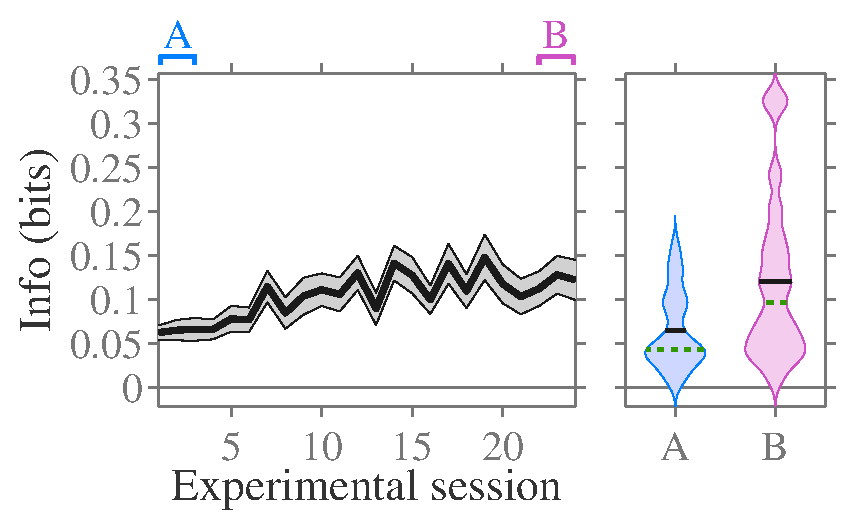
\includegraphics[scale=.45]{%
figs/info2/I_sessionwise_jack_v4_chmean20_s24,25,27-38,40-49_oc0_G_1bins_of_527ms_dr_pt_rmvet2_rmvms2_imscn_clhot.eps}}
    \hspace*{\fill}
    \caption{Information about the test stimulus contained in the firing rate during test presentation and its progression over training sessions.
% The mutual information with the test stimulus is taken for a spike timing based code for a \SI{20}{ms} window of spiking activity, sampled with the start of the window offset ($y$-axis) from \SI{0}{ms} up to \SI{500}{ms} after test stimulus onset.
% The sampling is in intervals of \SI{5}{ms}, so any 4 adjacent squares within each session are highly correlated.
% The recording session number for the data is given along the $x$-axis, and the number of days the animal has been trained for increases from left to right.
% Average mutual information across all the channels is denoted by the pseudo-colour of each of the rectangular patches, centred around the $(x,y)$ co-ordinate to which the measurement relates.
Main panels: the average over channels (\protect\subref{fig:info_sess_1x527_v1_blanco}~23 channels, \protect\subref{fig:info_sess_1x527_v1_jack}~$25$ channels, \protect\subref{fig:info_sess_1x527_v4_blanco}~30 channels, \protect\subref{fig:info_sess_1x527_v4_jack}~$20$ channels) with standard error over channels indicated by the shaded region.
Right hand panels: distribution over channels of the information contained in the first three sessions (\zonename{A}) versus last three sessions (\zonename{B}), with mean (solid black line) and median (dashed green line) over channels indicated.
The violin plot shows a Gaussian kernel density, using a bandwidth determined as described in \autoref{sec:info-methods}.
The \ac{PT} bias correction method was used, without further correction to the residual bias.
}
    \label{fig:info_sess_1x527}
\end{figure}


As described in \autoref{sec:pl_dprime_discuss}, the reduction of information witnessed for \ac{M1} \ac{V1} is most likely explained by the inescapable reduction of recording signal quality over time.
However, one channel had a large increase in information content against the trend observed for other channels on this electrode array (see \autoref{fig:info_sess_1x527_v1_blanco}, right panel).
This channel is one of a minority whose response profile changes completely between consecutive sessions, and so the sudden large increase in information is most likely due to a small movement in the electrode contact changing which neurons are measured in the data.
We address this discrepancy next.


%------------------------------------
\subsubsection{Removing inconsistent channels}

We noted that some channels were moving between sessions.
In general, it is just as likely for electrode contacts to move into locations where they are more informative as to move such that they are less informative.
However, to make the results more comparable across sessions, we chose to remove channels whose raster profile or overall firing rate in response to the \SI{30}{\percent} sample stimulus clearly changed from one session to the next.
We manually selected a small number of channels on this basis, and removed them from the analysis.
For each dataset, the number of channels included afterwards is indicated in \autoref{tab:nchannels_restricted}.


\begin{table}[bthp]
\begin{center}
\begin{tabular}{ccrr}
\toprule
Region  & Animal    & Channels before   & Channels after \\
\midrule
V1      & M1        & 23                & 14 \\
        & M2        & 25                & 20 \\
V4      & M1        & 30                & 25 \\
        & M2        & 20                & 18 \\
\bottomrule
\end{tabular}
\end{center}
\caption{Number of channels before and after restriction on the basis of consistent or smoothly changing firing rates across sessions.}
\label{tab:nchannels_restricted}
\end{table}


\begin{figure}[htbp]%
    \centering
    \hspace*{\fill}
    \subfloat[][\ac{M1} \ac{V1}.\label{fig:info_sess_1x527_restrictchn_v1_blanco}]{%
        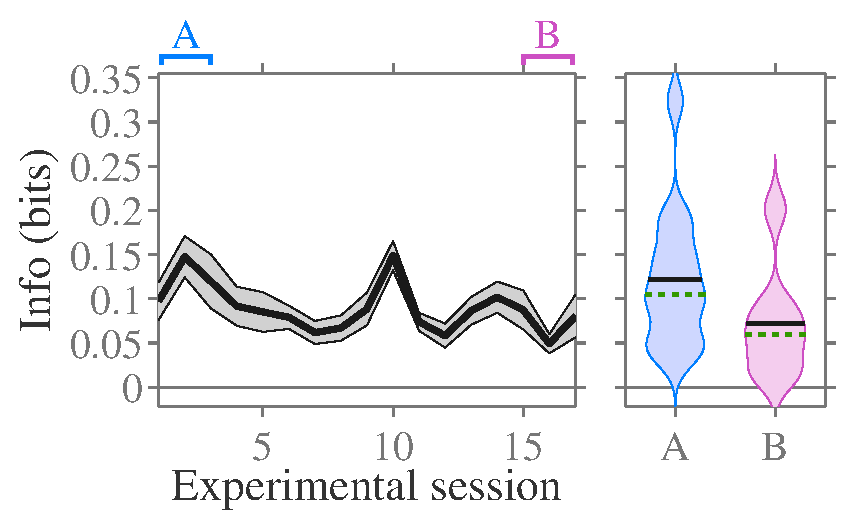
\includegraphics[scale=.45]{%
figs/info2/I_sessionwise_blanco_v1_chmean14_s343-359_oc0_G_1bins_of_527ms_dr_pt_rmvet2_rmvms2_imscn_clhot.eps}}
    \hspace*{\fill}\hspace{.2cm}\hspace*{\fill}
    \subfloat[][\ac{M2} \ac{V1}.\label{fig:info_sess_1x527_restrictchn_v1_jack}]{%
        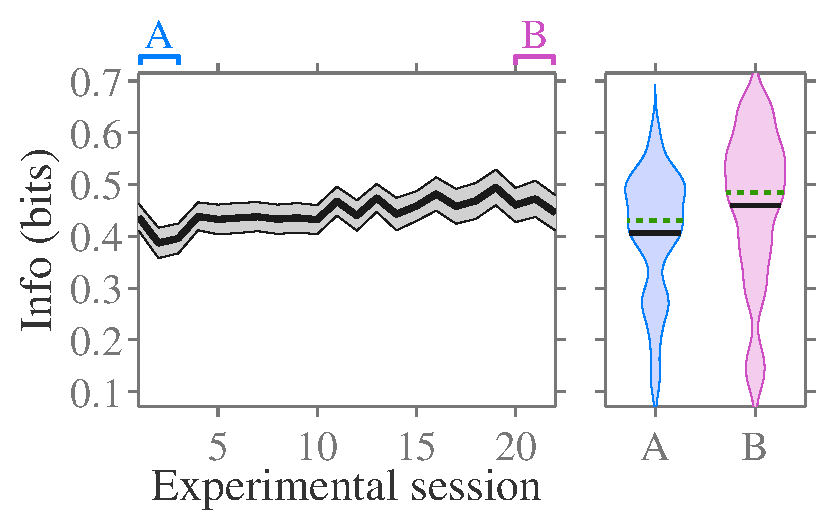
\includegraphics[scale=.45]{%
figs/info2/I_sessionwise_jack_v1_chmean20_s51-72_oc0_G_1bins_of_527ms_dr_pt_rmvet2_rmvms2_imscn_clhot.eps}}
    \hspace*{\fill}
    \\
    \hspace*{\fill}
    \subfloat[][\ac{M1} \ac{V4}.\label{fig:info_sess_1x527_restrictchn_v4_blanco}]{%
        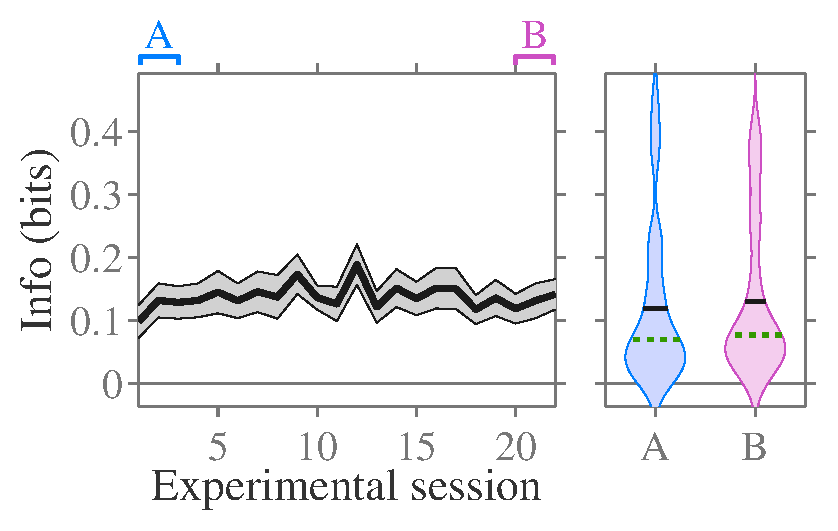
\includegraphics[scale=.45]{%
figs/info2/I_sessionwise_blanco_v4_chmean25_s307,308,311,313,314,317,318,320,321,329-341_oc0_G_1bins_of_527ms_dr_pt_rmvet2_rmvms2_imscn_clhot.eps}}
    \hspace*{\fill}\hspace{.2cm}\hspace*{\fill}
    \subfloat[][\ac{M2} \ac{V4}.\label{fig:info_sess_1x527_restrictchn_v4_jack}]{%
        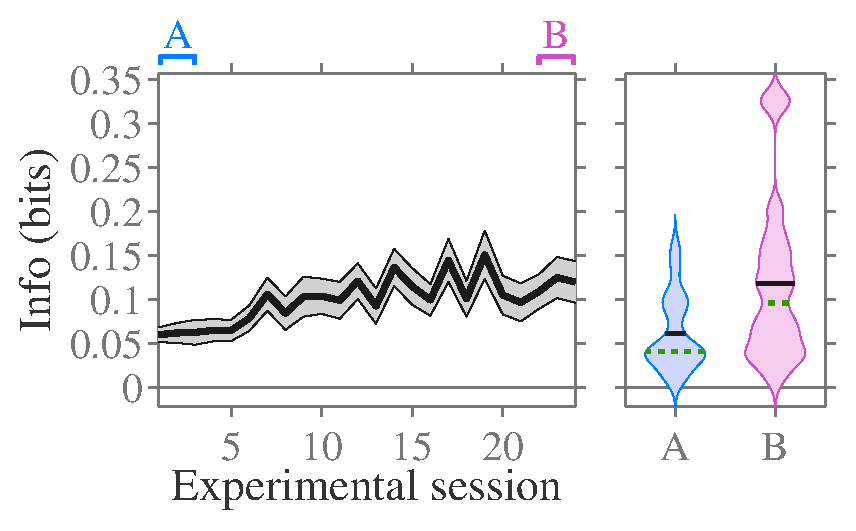
\includegraphics[scale=.45]{%
figs/info2/I_sessionwise_jack_v4_chmean18_s24,25,27-38,40-49_oc0_G_1bins_of_527ms_dr_pt_rmvet2_rmvms2_imscn_clhot.eps}}
    \hspace*{\fill}
    \caption{Information about the test stimulus contained in the firing rate during test presentation and its progression over training sessions.
Main panels: the average over channels (\protect\subref{fig:info_sess_1x527_restrictchn_v1_blanco}~$14$ channels, \protect\subref{fig:info_sess_1x527_restrictchn_v1_jack}~$20$ channels, \protect\subref{fig:info_sess_1x527_restrictchn_v4_blanco}~$25$ channels, \protect\subref{fig:info_sess_1x527_restrictchn_v4_jack}~$18$ channels) with standard error over channels indicated by the shaded region.
Right hand panels: distribution over channels of the information contained in the first three sessions (\zonename{A}) versus last three sessions (\zonename{B}), with mean (solid black line) and median (dashed green line) over channels indicated.
The violin plot shows a Gaussian kernel density, using a bandwidth determined as described in \autoref{sec:info-methods}.
The \ac{PT} bias correction method was used, without further correction to the residual bias.
}
    \label{fig:info_sess_1x527_restrictchn}
\end{figure}

% blanco v1 1x527.00ms
% dr pt
% same bandwidth bw = 0.018561 used for all cols
% h=1.000000  p=0.014856=1.485642e-02   delta = -0.049242+/-0.017549 = -40.514232%+/-14.587530%
%
% jack v1 1x527.00ms
% dr pt
% same bandwidth bw = 0.033931 used for all cols
% h=1.000000  p=0.000970=9.696090e-04   delta = +0.052784+/-0.013545 = +12.980690%+/-4.272728%
%
% blanco v4 1x527.00ms
% dr pt
% same bandwidth bw = 0.033252 used for all cols
% h=0.000000  p=0.556266=5.562658e-01   delta = +0.010819+/-0.018130 = +9.059702%+/-15.387211%
%
% jack v4 1x527.00ms
% dr pt
% same bandwidth bw = 0.012428 used for all cols
% h=1.000000  p=0.001046=1.046127e-03   delta = +0.056465+/-0.014315 = +91.889667%+/-23.318749%

Besides the channel for \ac{M1} \ac{V1} with an aberrantly large increase in information mentioned above, there is little impact on the results (\autoref{fig:info_sess_1x527_restrictchn}) compared with previously (\autoref{fig:info_sess_1x527}).
For this dataset, \ac{M1} \ac{V1}, the removal of the outlier means the reduction in information over time is now statistically significant (\SI{-0.049\pm0.018}{bits} or \SI{-41\pm15}{\percent}, $p=0.015$).
For the other datasets, there were no notable changes.


%------------------------------------
\subsubsection{Correcting for stimulus class imbalance}
\label{sec:pl_class_imbalance}

As mentioned in \autoref{sec:pl_task}, the stimulus presentation procedure was to include a fixed number of repetitions of each stimulus in a block of trials and present them in a random order.
At the end of each block, additional trials were presented for stimuli which the subject responded to incorrectly.
Since stimuli with a contrast far from the pedestal contrast of \SI{30}{\percent} are much easier for the subject, trials which were repeated at the end of the block were not uniformly distributed across the stimuli.
Overall, this means that harder stimuli close to \SI{30}{\percent} contrast are presented more often than the easier stimuli.

When computing the amount of information about the stimulus contained in the animal's response, we do not need to have a uniform distribution across stimuli.
However, the subject becomes better at the task with training, and the change in relative performance is not uniform across sessions.
Performance on the easiest stimuli is high at the beginning of training and has little room for further improvements.
The hardest stimuli are very challenging, and performance on these does not rise much above chance even after training.
The increase in performance is highest for the stimuli of intermediate difficulty, and so since their first-try success rate improves they represent a smaller proportion of the total trials after training.

FIGURE SHOWING CHANGE IN CLASS BALANCE OVER TIME

Changes in the distribution of classes between sessions can impact our analysis in two ways.
Firstly, as described \autoref{eq:info} the amount of information between stimulus, $\SET{S}$, and response, $\SET{R}$, is dependent on the entropy of the stimulus, $\HH(\SET{S})$.
As the distribution of stimulus classes moves closer to uniform, the stimulus entropy increases.
Since our stimulus distribution becomes flatter with training, this may cause an the measured information to become inflated as training progresses.
Secondly, the proportion trials which are in the easier categories increases over time.
These stimuli will have the most distinguishable responses, and their increasing prevalence in the dataset may also produce an artificial increase in information with training.

We corrected the class imbalance on a session-by-session basis by subsampling the trials for more frequent stimulus classes down to the frequency of the least common stimulus class.
The trials included in the subsample were selected at random across the set of trials for each stimulus, without replacement.


\begin{figure}[htbp]%
    \centering
    \hspace*{\fill}
    \subfloat[][\ac{M1} \ac{V1}.\label{fig:info_sess_1x527_balanced_v1_blanco}]{%
        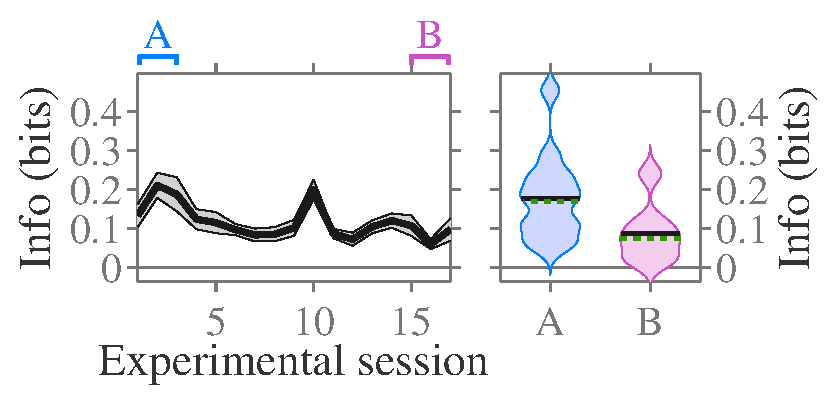
\includegraphics[scale=.45]{%
figs/info2/I_sessionwise_blanco_v1_chmean14_s343-359_oc0_Gbalanced_1bins_of_527ms_dr_pt_rmvet2_rmvms2_imscn_clhot.eps}}
    \hspace*{\fill}\hspace{.2cm}\hspace*{\fill}
    \subfloat[][\ac{M2} \ac{V1}.\label{fig:info_sess_1x527_balanced_v1_jack}]{%
        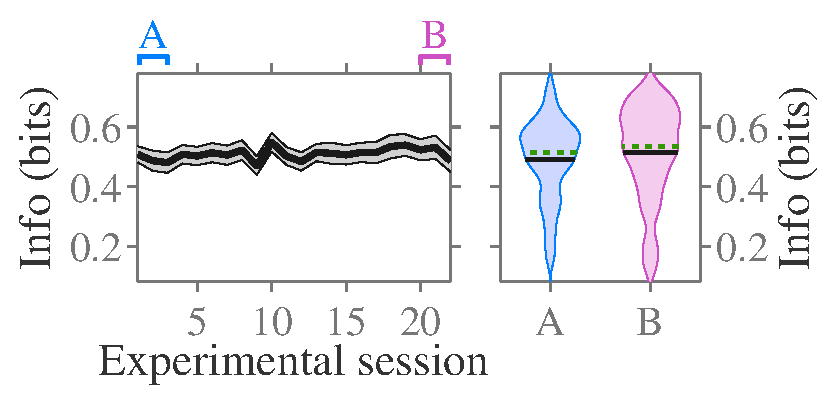
\includegraphics[scale=.45]{%
figs/info2/I_sessionwise_jack_v1_chmean20_s51-72_oc0_Gbalanced_1bins_of_527ms_dr_pt_rmvet2_rmvms2_imscn_clhot.eps}}
    \hspace*{\fill}
    \\
    \hspace*{\fill}
    \subfloat[][\ac{M1} \ac{V4}.\label{fig:info_sess_1x527_balanced_v4_blanco}]{%
        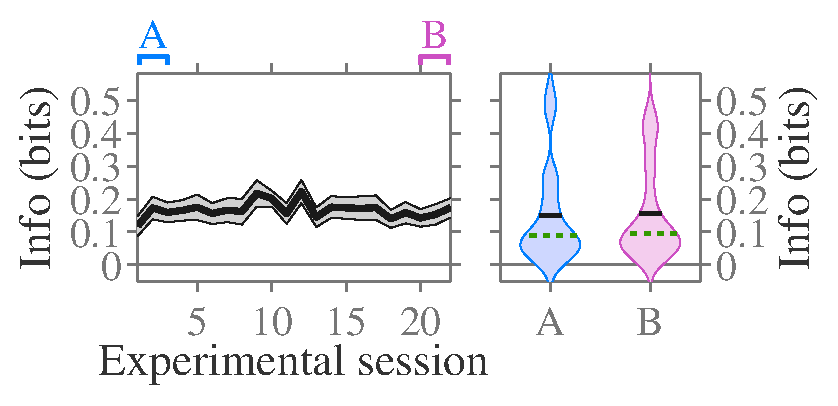
\includegraphics[scale=.45]{%
figs/info2/I_sessionwise_blanco_v4_chmean25_s307,308,311,313,314,317,318,320,321,329-341_oc0_Gbalanced_1bins_of_527ms_dr_pt_rmvet2_rmvms2_imscn_clhot.eps}}
    \hspace*{\fill}\hspace{.2cm}\hspace*{\fill}
    \subfloat[][\ac{M2} \ac{V4}.\label{fig:info_sess_1x527_balanced_v4_jack}]{%
        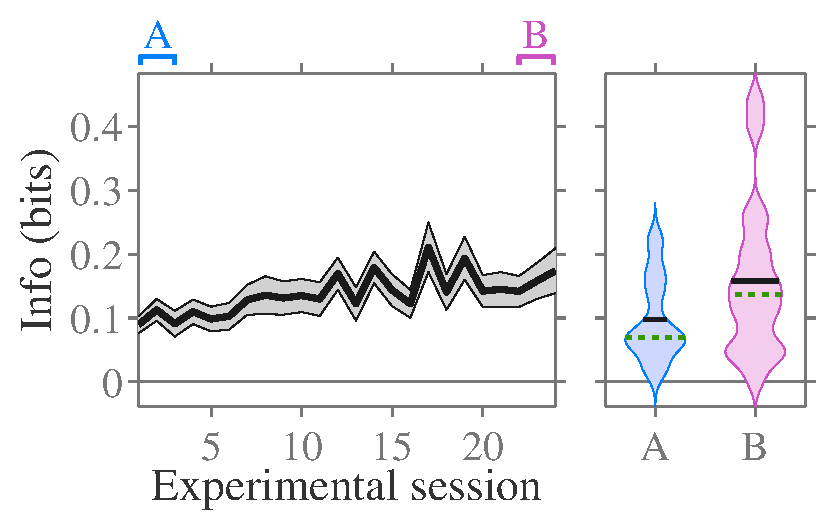
\includegraphics[scale=.45]{%
figs/info2/I_sessionwise_jack_v4_chmean18_s24,25,27-38,40-49_oc0_Gbalanced_1bins_of_527ms_dr_pt_rmvet2_rmvms2_imscn_clhot.eps}}
    \hspace*{\fill}
    \caption{Information about the test stimulus contained in the firing rate during test presentation and its progression over training sessions, after correcting for the stimulus class balance in each session.
Main panels: the average over channels (\protect\subref{fig:info_sess_1x527_balanced_v1_blanco}~$14$ channels, \protect\subref{fig:info_sess_1x527_balanced_v1_jack}~$20$ channels, \protect\subref{fig:info_sess_1x527_balanced_v4_blanco}~$25$ channels, \protect\subref{fig:info_sess_1x527_balanced_v4_jack}~$18$ channels) with standard error over channels indicated by the shaded region.
Right hand panels: distribution over channels of the information contained in the first three sessions (\zonename{A}) versus last three sessions (\zonename{B}), with mean (solid black line) and median (dashed green line) over channels indicated.
The violin plot shows a Gaussian kernel density, using a bandwidth determined as described in \autoref{sec:info-methods}.
The \ac{PT} bias correction method was used, without further correction to the residual bias.
}
    \label{fig:info_sess_1x527_balanced}
\end{figure}

% blanco v1 1x527.00ms
% dr pt
% same bandwidth bw = 0.02234 used for all cols
% h=1.000000  p=0.001794=1.794017e-03   delta = -0.089123+/-0.022797 = -50.472174%+/-13.226381%
%
% jack v1 1x527.00ms
% dr pt
% same bandwidth bw = 0.038202 used for all cols
% h=0.000000  p=0.179003=1.790031e-01   delta = +0.022181+/-0.015896 = +4.511570%+/-4.419345%
%
% blanco v4 1x527.00ms
% dr pt
% same bandwidth bw = 0.038581 used for all cols
% h=0.000000  p=0.779391=7.793914e-01   delta = +0.006273+/-0.022144 = +4.185196%+/-15.076193%
%
% jack v4 1x527.00ms
% dr pt
% same bandwidth bw = 0.018676 used for all cols
% h=1.000000  p=0.004131=4.130838e-03   delta = +0.060078+/-0.018145 = +61.470204%+/-18.627960%


Overall, we find the amount of information increases when the class imbalance is for (compare the y-scales of \autoref{fig:info_sess_1x527_balanced} with those of \autoref{fig:info_sess_1x527_restrictchn}).
This is because the stimulus entropy, $\HH(\SET{S})$, has increased when the stimulus distribution became uniform.

As anticipated, correcting for changes in the class balance over time reduces the relative increase in information between the beginning and end of training.
For \ac{V1}, the reduction in information with time seen in \ac{M1} is increased (\SI{-0.089\pm0.023}{bits} or \SI{-50\pm13}{\percent}, $p=0.0018$) and the increase in information for \ac{M2} is no longer statistically significant (\SI{+0.022\pm0.016}{bits} or \SI{+4.5\pm4.4}{\percent}, $p=0.18$).
For \ac{V4}, the outcomes stand unchanged even though the relative change in information is reduced
(\ac{M1}: \SI{+0.006\pm0.022}{bits} or \SI{+4\pm15}{\percent}, $p=0.78$; \ac{M2}: \SI{+0.060\pm0.018}{bits} or \SI{+61\pm19}{\percent}, $p=0.004$).


%------------------------------------
\subsubsection{Defending against changes in session duration}

A large amount of session-to-session variability in the measurements was observed in our results (\autoref{fig:info_sess_1x527}).
Further investigation revealed that this variability was due to changes in the duration of each session --- some sessions contain $5$ times as many trials as others.

Although we were utilising the \ac{PT} bias correction technique, this typically requires $4$ trials per response for each stimulus condition to be completely effective \citep{Panzeri2007}.
When analysing the amount of information contained in the overall firing rate, the cardinality of the set of spike counts per channel ranges from N to M.
The number of trials per session (including all 14 stimulus conditions) ranges from N to M. (250 to 1250, approx)
Consequently, the number of trials per stimulus ranges from N to M.
After correcting for the stimulus class imbalance, the effective number of trials per session ranges from N to M.

This shortage of trials per stimulus condition results means the \ac{PT} bias correction method underestimates the bias for the shorter sessions, leading to an overestimate in the reported information.
This is illustrated in \autoref{fig:I_vs_invN}, where we compare with the estimated information with the reciprocal number of trials, $\nicefrac{1}{N}$, and find a linear correlation.
This is in keeping with the literature, since $\I_{\text{measured}}$ is known to be proportional to $\nicefrac{1}{N}$ if no bias correction is performed \citep{Treves1995}.


\begin{figure}[htbp]
    \centering
    \hspace*{\fill}
    \subfloat[][\ac{M1} \ac{V1}.\label{fig:I_vs_invN_v1_blanco}]{%
        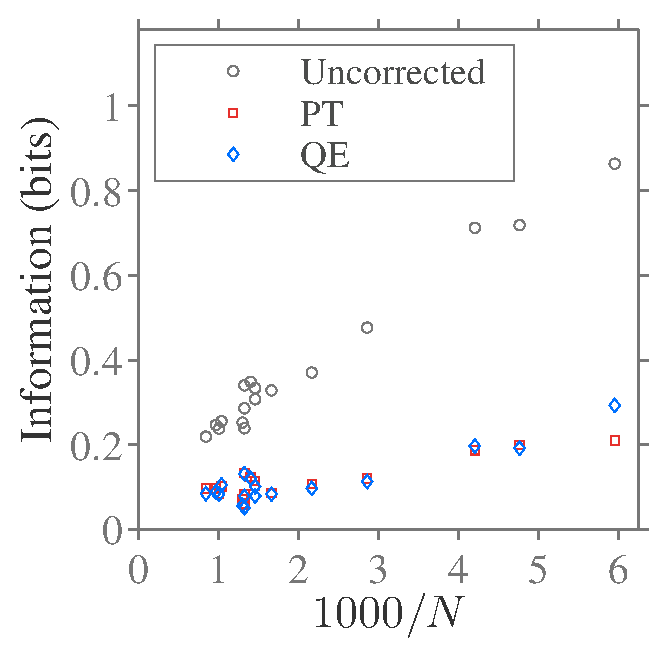
\includegraphics[scale=.45]{%
figs/info2/ntrials_I_vs_invN_combindivpap_leg_blanco_v1_14chn_Gbalanced_1bins_of_527ms.eps}}
    \hspace*{\fill}\hspace{.2cm}\hspace*{\fill}
    \subfloat[][\ac{M2} \ac{V1}.\label{fig:I_vs_invN_v1_jack}]{%
        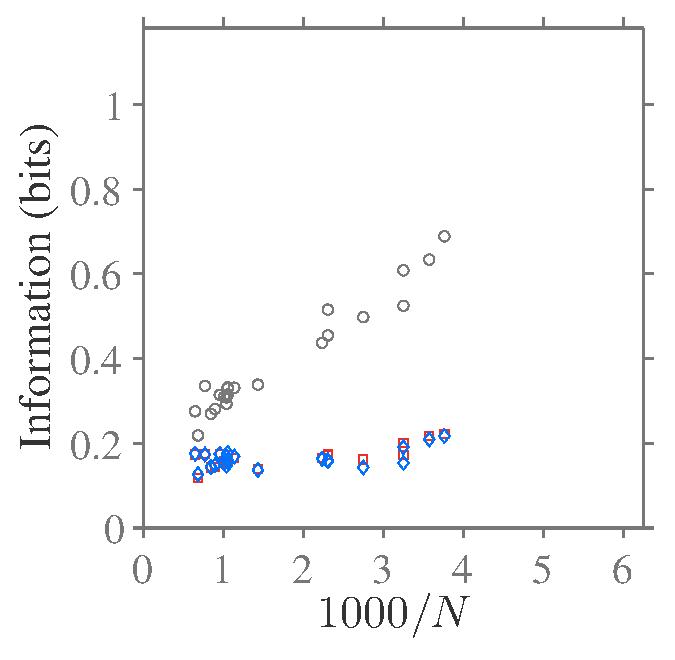
\includegraphics[scale=.45]{%
figs/info2/ntrials_I_vs_invN_combindivpap_blanco_v4_25chn_Gbalanced_1bins_of_527ms.eps}}
    \hspace*{\fill}
    \\
    \hspace*{\fill}
    \subfloat[][\ac{M1} \ac{V4}.\label{fig:I_vs_invN_v4_blanco}]{%
        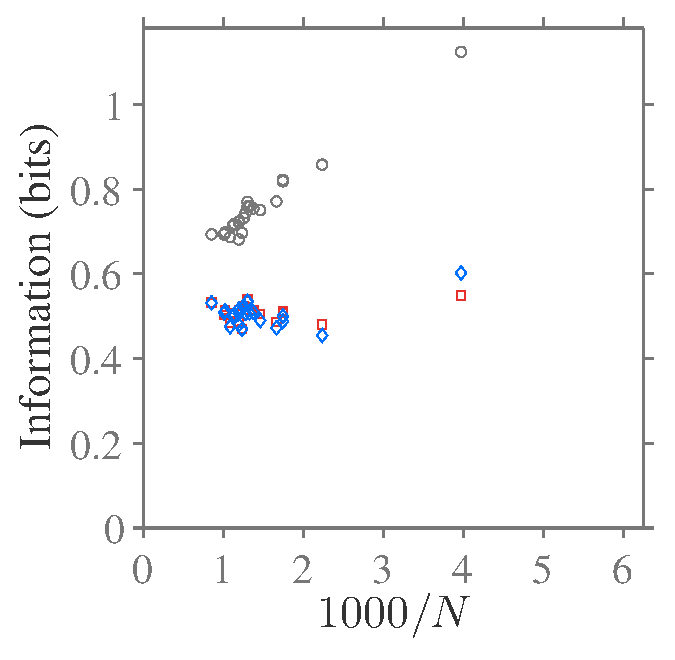
\includegraphics[scale=.45]{%
figs/info2/ntrials_I_vs_invN_combindivpap_jack_v1_20chn_Gbalanced_1bins_of_527ms.eps}}
    \hspace*{\fill}\hspace{.2cm}\hspace*{\fill}
    \subfloat[][\ac{M2} \ac{V4}.\label{fig:I_vs_invN_v4_jack}]{%
        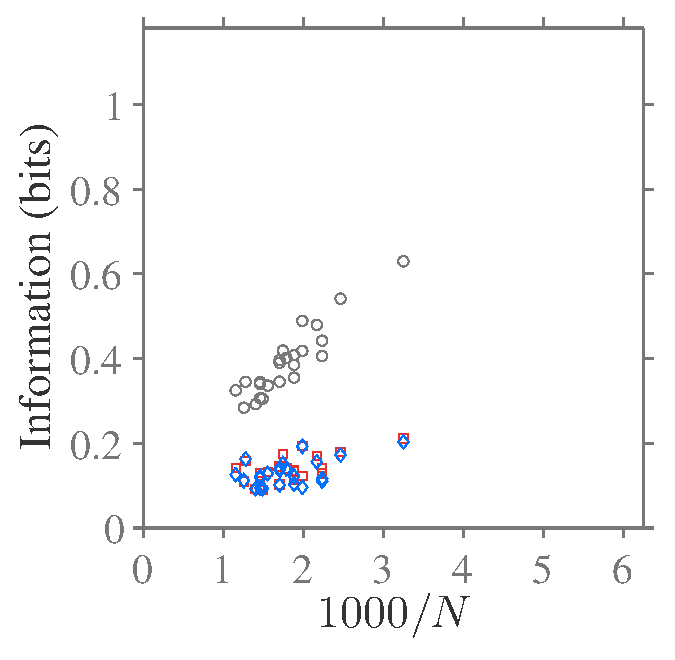
\includegraphics[scale=.45]{%
figs/info2/ntrials_I_vs_invN_combindivpap_jack_v4_18chn_Gbalanced_1bins_of_527ms.eps}}
    \hspace*{\fill}
    \caption{Distribution of measured information as a function of $\nicefrac{1}{N}$, where $N$ is the number of trials in the session.
Results are shown both without correcting for the finite measurement bias (grey circles), using \ac{PT} bias correction (red squares), and using \ac{QE} bias correction (blue diamonds).
Information was computed after using subsampling to address the stimulus class imbalance (see \autoref{sec:pl_class_imbalance}), and this is reflected in the value of $N$.
}
    \label{fig:IvN}
    \label{fig:I_vs_invN}
\end{figure}


There are several potential ways we can correct for the change in bias incurred by the changes in number of trials.
\begin{itemize}
\item Subsample all sessions down to the same number of trials.
\item Use bootstrapping, shuffling response against stimuli at random, to estimate and subtract the residual bias.
\item Group together stimuli above and below \SI{30}{\percent} contrast so we only two conditions each with $\approx7$ times more trials.
\item Group together trials across consecutive sessions so we have the same number of trials in each information computation step.
\end{itemize}

The first method is clearly undesirable, since we would be throwing away most of our data and knowingly operating in the regime where the bias correction method breaks down for all sessions instead of only a few.
In such a scenario, the bias on the estimated information would be larger than the actual information and our comparison across sessions would have little validity.
Instead, we focus on the three other more practical methods, whose outcomes are described below.


%------------------------------------
 \subsubsection{Bootstrap correction}

Shuffling the responses across stimuli destroys the information contained in the response about the stimulus.
By performing such shuffling and computing the amount of information between the randomly paired labels, we can estimate the bias \citep{Optican1991}.
Using this in conjunction with a bias correction technique such as \ac{PT} both when performing the original and bootstrapped information calculation allows us to estimate the residual bias after on the corrected value.
As described in \autoref{sec:info-bias} and by \citet{Panzeri1996}, this will typically lead to an overestimate of the bias.
However, since our residual bias will be significantly reduced beforehand due to the \ac{PT} technique, the overestimation is on a much smaller residual bias and impacts the results less.

\begin{figure}[htbp]
    \centering
    \hspace*{\fill}
    \subfloat[][\ac{M1} \ac{V1}.\label{fig:I_vs_invN_btsp_v1_blanco}]{%
        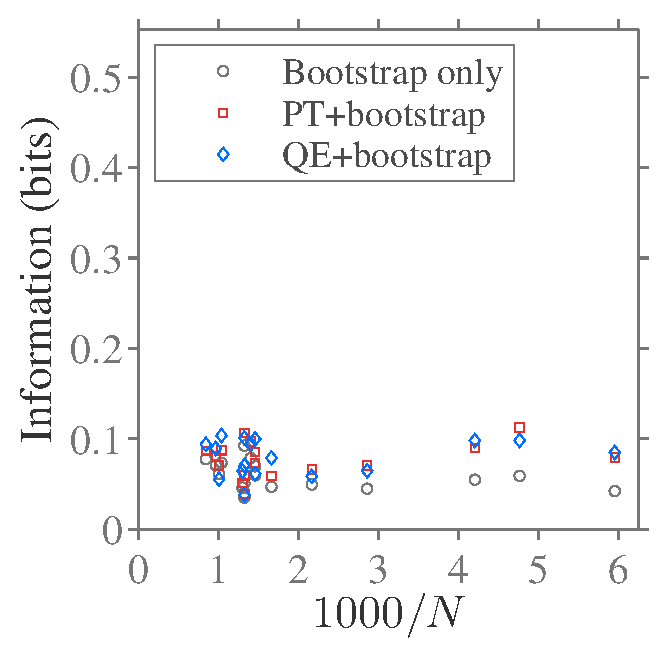
\includegraphics[scale=.45]{%
figs/info2/ntrials_I_vs_invN_combindivpap_leg_blanco_v1_14chn_Gbalanced_1bins_of_527ms_btsp20.eps}}
    \hspace*{\fill}\hspace{.2cm}\hspace*{\fill}
    \subfloat[][\ac{M2} \ac{V1}.\label{fig:I_vs_invN_btsp_v1_jack}]{%
        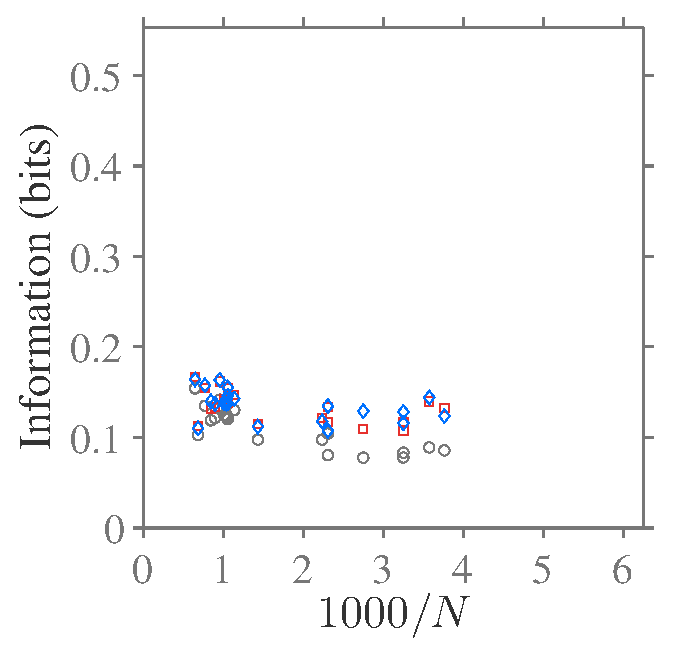
\includegraphics[scale=.45]{%
figs/info2/ntrials_I_vs_invN_combindivpap_blanco_v4_25chn_Gbalanced_1bins_of_527ms_btsp20.eps}}
    \hspace*{\fill}
    \\
    \hspace*{\fill}
    \subfloat[][\ac{M1} \ac{V4}.\label{fig:I_vs_invN_btsp_v4_blanco}]{%
        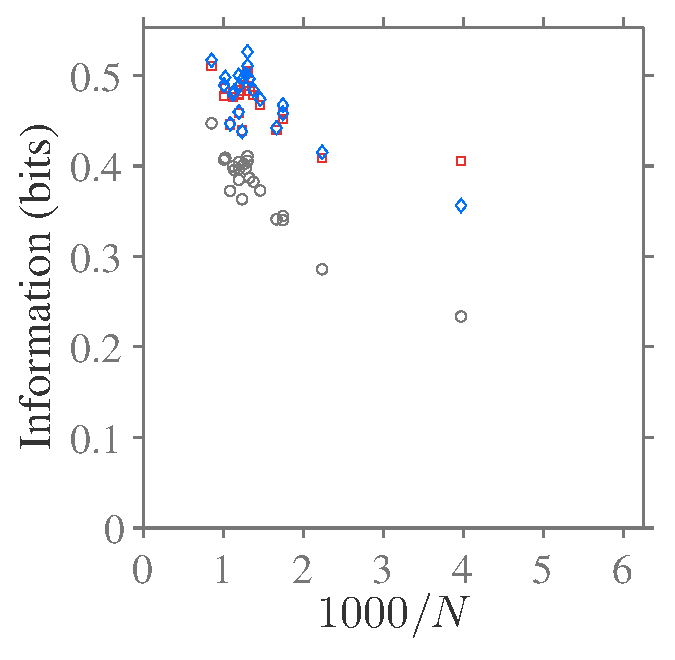
\includegraphics[scale=.45]{%
figs/info2/ntrials_I_vs_invN_combindivpap_jack_v1_20chn_Gbalanced_1bins_of_527ms_btsp20.eps}}
    \hspace*{\fill}\hspace{.2cm}\hspace*{\fill}
    \subfloat[][\ac{M2} \ac{V4}.\label{fig:I_vs_invN_btsp_v4_jack}]{%
        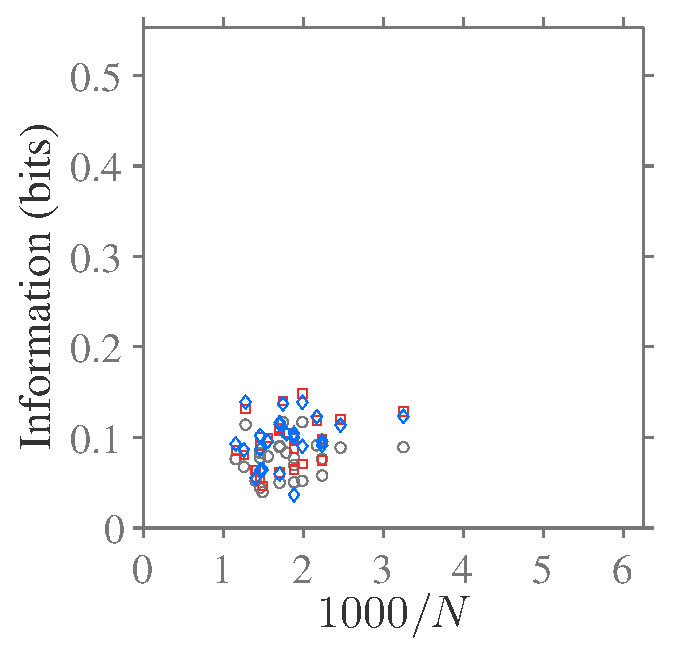
\includegraphics[scale=.45]{%
figs/info2/ntrials_I_vs_invN_combindivpap_jack_v4_18chn_Gbalanced_1bins_of_527ms_btsp20.eps}}
    \hspace*{\fill}
    \caption{Distribution of measured information as a function of $\nicefrac{1}{N}$, where $N$ is the number of trials in the session.
Results are shown with bias correction either achieved solely from subtracting the information contained in response-shuffled copies of the data (grey circles), or by combining this with a better principled bias correction technique (\ac{PT}, red squares; \ac{QE}, blue diamonds).
Information was computed after using subsampling to address the stimulus class imbalance (see \autoref{sec:pl_class_imbalance}), and this is reflected in the value of $N$.
}
    \label{fig:I_vs_invN_btsp}
\end{figure}

We find that using bootstrapping for the bias correction does indeed overestimate the bias, resulting in a negative correlation between information and $\nicefrac{1}{N}$.
This effect is particularly dominant for the \ac{M1} \ac{V4} dataset (see \autoref{fig:I_vs_invN_btsp_v4_blanco}).

%------------------------------------
 \subsubsection{Grouping stimuli together}

During the experiment, the subject is tasked with determining whether the stimulus contrast is higher or lower than the \SI{30}{\percent} sample stimulus presented at the start of each trial.
As a consequence of this, the subject does not need to learn exactly what stimulus is on screen, only whether the stimulus is in the half above or below \SI{30}{\percent} contrast.
For instance, since the target output is the same for \SI{31}{\percent} and \SI{32}{\percent} contrast stimuli, there is no need for the subject to discriminate between them, but there is motivation for the subject to learn to discriminate between these and the \SI{29}{\percent} contrast stimulus.


\begin{figure}[htbp]
    \centering
    \hspace*{\fill}
    \subfloat[][\ac{M1} \ac{V1}.\label{fig:I_vs_invN_target-group_v1_blanco}]{%
        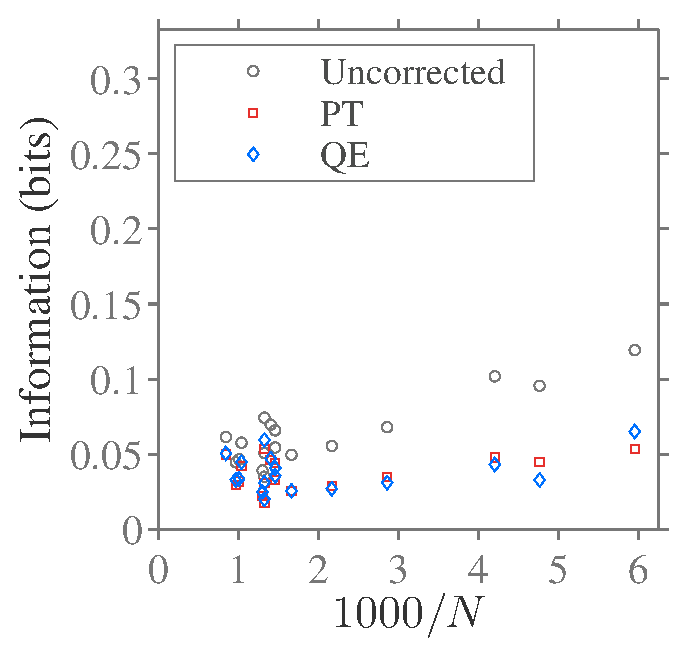
\includegraphics[scale=.45]{%
figs/info2/ntrials_I_vs_invN_combindivpap_leg_blanco_v1_14chn_Gclass-group-balanced_1bins_of_527ms.eps}}
    \hspace*{\fill}\hspace{.2cm}\hspace*{\fill}
    \subfloat[][\ac{M2} \ac{V1}.\label{fig:I_vs_invN_target-group_v1_jack}]{%
        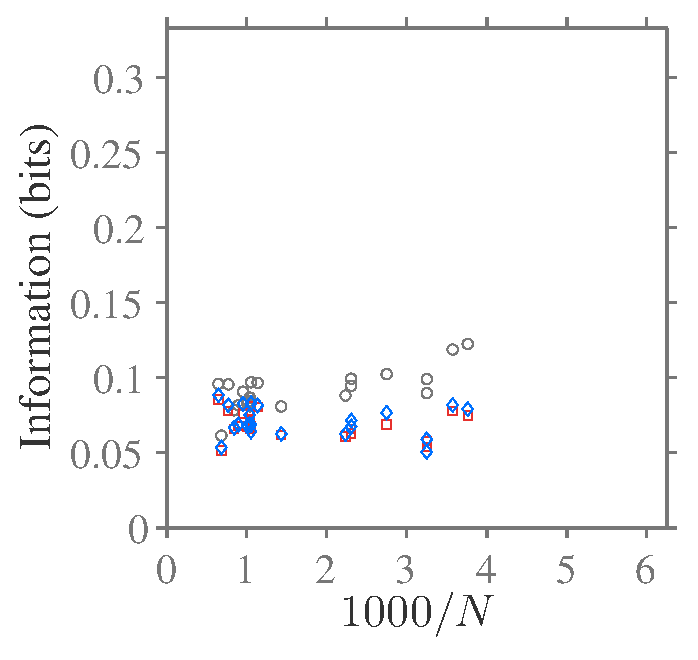
\includegraphics[scale=.45]{%
figs/info2/ntrials_I_vs_invN_combindivpap_blanco_v4_25chn_Gclass-group-balanced_1bins_of_527ms.eps}}
    \hspace*{\fill}
    \\
    \hspace*{\fill}
    \subfloat[][\ac{M1} \ac{V4}.\label{fig:I_vs_invN_target-group_v4_blanco}]{%
        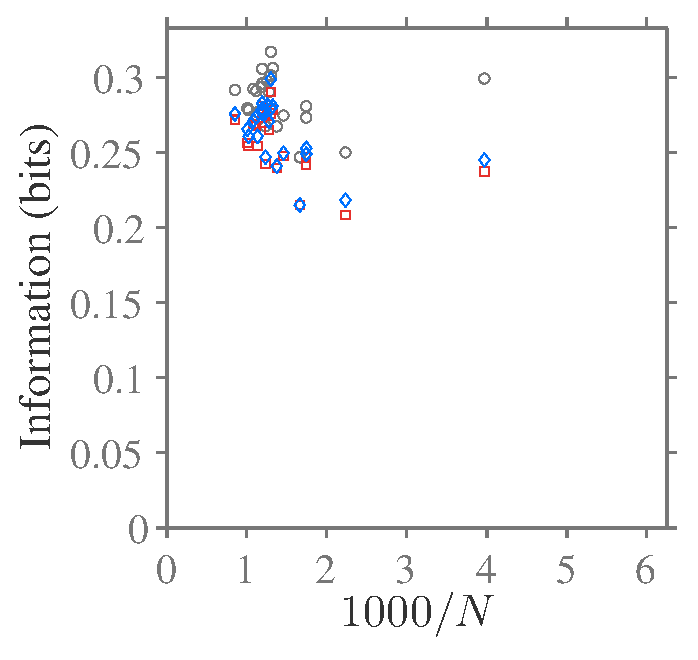
\includegraphics[scale=.45]{%
figs/info2/ntrials_I_vs_invN_combindivpap_jack_v1_20chn_Gclass-group-balanced_1bins_of_527ms.eps}}
    \hspace*{\fill}\hspace{.2cm}\hspace*{\fill}
    \subfloat[][\ac{M2} \ac{V4}.\label{fig:I_vs_invN_target-group_v4_jack}]{%
        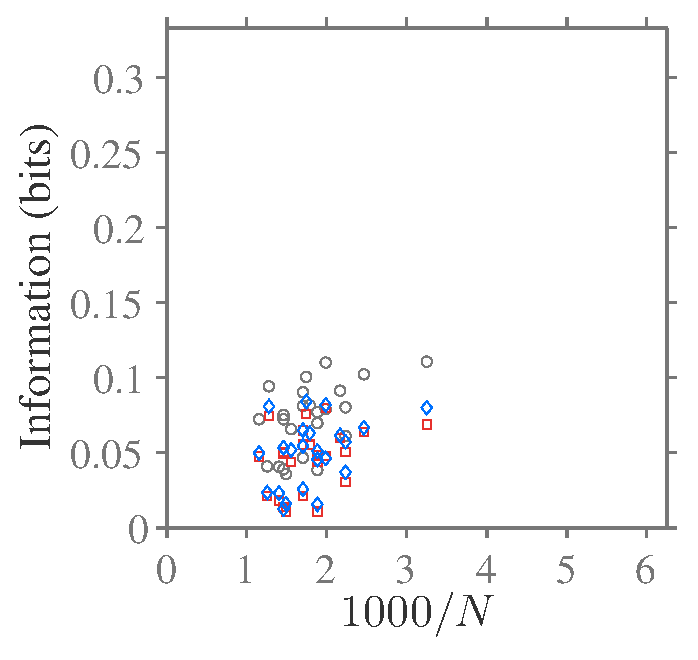
\includegraphics[scale=.45]{%
figs/info2/ntrials_I_vs_invN_combindivpap_jack_v4_18chn_Gclass-group-balanced_1bins_of_527ms.eps}}
    \hspace*{\fill}
    \caption{Distribution of measured information as a function of $\nicefrac{1}{N}$, where $N$ is the number of trials in the session.
Results are shown both without correcting for the finite measurement bias (grey circles), using \ac{PT} bias correction (red squares), and using \ac{QE} bias correction (blue diamonds).
Information was computed after using subsampling to address the stimulus class imbalance (see \autoref{sec:pl_class_imbalance}), and this is reflected in the value of $N$.
}
    \label{fig:I_vs_invN_target-group}
\end{figure}

Grouping the stimuli together in this manner reduces the total amount of information which is measured (compare the $y$-axis scale bars of \autoref{fig:I_vs_invN_target-group} with \autoref{fig:I_vs_invN}).
The fraction of information encoded in the neural response which is task-specific is investigated in more detail in \autoref{sec:task-info}.
For now, we are only concerned with whether we can prevent differences in information estimation between sessions due to a shortage of trials per stimulus by grouping together the stimuli into two categories.

As anticipated, using only two stimulus classes to increase the number of trials per stimulus class greatly reduces the residual bias after \ac{PT} bias correction.
This is witnessed in the reduced correlation between estimated information and $\nicefrac{1}{N}$ seen in \autoref{fig:I_vs_invN_target-group}.

%------------------------------------
 \subsubsection{Trial-wise analysis}

We now consider what happens if we group together trials from multiple sessions into a single block and analyse them together.
Doing so allows us overcome the difference in bias between sessions, since the same number of trials would be used in each block and this can be set large enough to ensure we are in the correct domain for bias correction perform adequately.
There are typically no more than $25$ different firing rates for any single channel, so we grouped together $100$ trials of each stimulus condition.

Using this methodology, we focus on the subject's performance as a function of the number of trials which they have completed since the beginning of the experiment, irrespective of how many training sessions these trials are spread across.
Therefore, such a technique makes sense if we consider learning to occur during sessions and not to occur between them.
However, such a view is in contrast with the hypothesis that one of the important functions of sleep is to facilitate consolidation of memories and learning from during the day.
Should this be an important contributor towards perceptual learning, one would expect the breaks between sessions not to be irrelevant but to instead enable an increase in performance even without exposure to the training stimuli.


\begin{figure}[htbp]%
    \centering
    \hspace*{\fill}
    \subfloat[][\ac{M1} \ac{V1}.\label{fig:info_trial_1x527_balanced_v1_blanco}]{%
        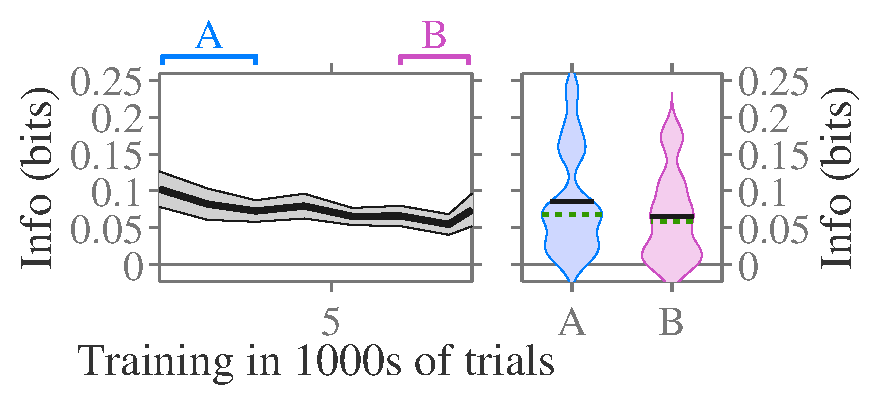
\includegraphics[scale=.45]{%
figs/info2/I_trialwise_blanco_v1_chmean14_s343-354,355.1,355.2,356-359_tp4_1bins_of_527ms_dr_pt_oc0_Gbalanced_test_tc5-5-20,22-3-28,32,35-5-50,60,90_nt1400_ts1400_rmvet2_rmvms2_imscn_clhot.eps}}
    \hspace*{\fill}\hspace{.2cm}\hspace*{\fill}
    \subfloat[][\ac{M2} \ac{V1}.\label{fig:info_trial_1x527_balanced_v1_jack}]{%
        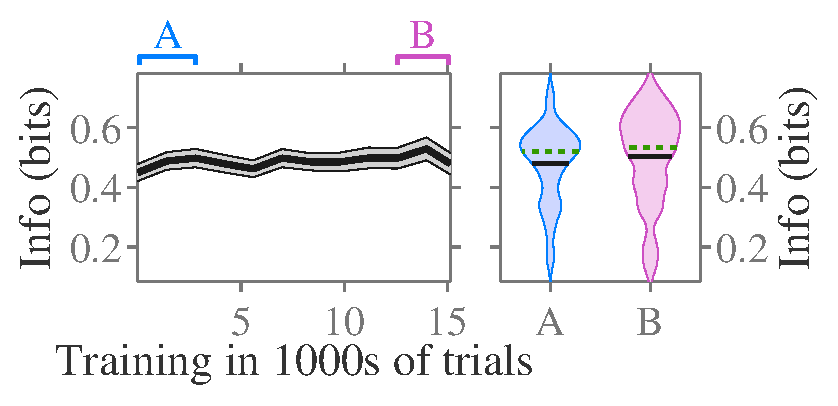
\includegraphics[scale=.45]{%
figs/info2/I_trialwise_jack_v1_chmean20_s51-72_tp4_1bins_of_527ms_dr_pt_oc0_Gbalanced_test_tc5-5-20,22-3-28,32,35-5-50,60,90_nt1400_ts1400_rmvet2_rmvms2_imscn_clhot.eps}}
    \hspace*{\fill}
    \\
    \hspace*{\fill}
    \subfloat[][\ac{M1} \ac{V4}.\label{fig:info_trial_1x527_balanced_v4_blanco}]{%
        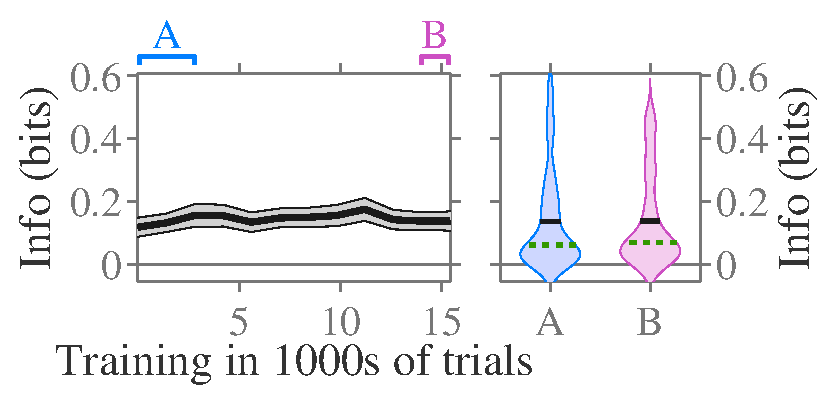
\includegraphics[scale=.45]{%
figs/info2/I_trialwise_blanco_v4_chmean25_s307,308,311,313,314,317,318,320,321,329-341_tp4_1bins_of_527ms_dr_pt_oc0_Gbalanced_test_tc10-5-25,27-29,31-33,35,40-10-60_nt1400_ts1400_rmvet2_rmvms2_imscn_clhot.eps}}
    \hspace*{\fill}\hspace{.2cm}\hspace*{\fill}
    \subfloat[][\ac{M2} \ac{V4}.\label{fig:info_trial_1x527_balanced_v4_jack}]{%
        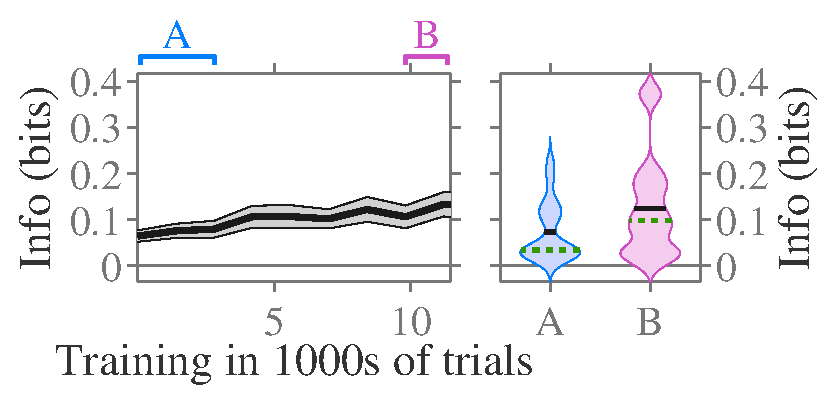
\includegraphics[scale=.45]{%
figs/info2/I_trialwise_jack_v4_chmean18_s24,25,27-38,40-49_tp4_1bins_of_527ms_dr_pt_oc0_Gbalanced_test_tc10-5-25,27-29,31-33,35,40-10-60_nt1400_ts1400_rmvet2_rmvms2_imscn_clhot.eps}}
    \hspace*{\fill}
    \caption{Information about the test stimulus contained in the firing rate during test presentation and its progression over training sessions, estimated across blocks of $100$ consecutive trials of each stimulus class taken by merging consecutive sessions together to accumulate sufficiently many trials.
Main panels: the average over channels (\protect\subref{fig:info_trial_1x527_balanced_v1_blanco}~$14$ channels, \protect\subref{fig:info_trial_1x527_balanced_v1_jack}~$20$ channels, \protect\subref{fig:info_trial_1x527_balanced_v4_blanco}~$25$ channels, \protect\subref{fig:info_trial_1x527_balanced_v4_jack}~$18$ channels) with standard error over channels indicated by the shaded region.
Right hand panels: distribution over channels of the information contained in the first three blocks of $1400$ trials (\zonename{A}) versus last three blocks (\zonename{B}), with mean (solid black line) and median (dashed green line) over channels indicated.
The violin plot shows a Gaussian kernel density, using a bandwidth determined as described in \autoref{sec:info-methods}.
The \ac{PT} bias correction method was used, without further correction to the residual bias.
The stimulus class imbalance was address on a session-by-session basis by subsampling as described previously (\autoref{sec:pl_class_imbalance}) before merging sessions together.
}
    \label{fig:info_trial_1x527_balanced}
\end{figure}


Since we performed the spike extraction such that the spontaneous firing rate is held constant across sessions for each channel, the firing rate during stimulus presentation is comparable between sessions.
This means it is plausible that, when decoding the information, the extracted firing rate corresponding to the stimuli could be similar across consecutive sessions.

We find that grouping trials together in this way smooths out the problems with inter-session changes in residual bias on the information estimate.
But because of both changes in neural connectivity and small movement in the electrode contacts between sessions, the neural code is not guaranteed to be the same between sessions.
Indeed, we observed a peak in the estimated information corresponding to longer sessions where the trial sample size is smaller than or a similar size to the number of trials grouped together in each block.
For this reason, it is prudent not to proceed with such a methodology.


%------------------------------------------------------------------------------
\subsection{Task-pertinent information}
% \subsection{Comparing information about the stimulus with task-relevant information}
\label{sec:task-info}

Show for the animal's response

Show for the neural response

%------------------------------------------------------------------------------
\subsection{Information versus firing rate integration window duration}


%------------------------------------------------------------------------------
\subsection{Information in spike timing}



%------------------------------------------------------------------------------
\subsection{Trial-based analysis}

To counter the correlation between measured information and number of trials, an obvious solution is to use the same number of trials for every computation.
We now consider how many trials should be taken at once to obtain a reasonably reliable estimate.

Some rules-of-thumb for the number of trials are offered by \citep{Panzeri2007}.
Let $\overline{R}$ denote the number of possible response codes.
Then, for the bias-uncorrected estimate of mutual information, we need to have at least $N_S \ge 2^{32} \, \overline{R}$ trials per stimulus,
whilst if the \ac{PT} or \ac{QE} bias correction methods are applied, we only need $N_S > 2 \, \overline{R}$.

% The spike detection software was set to only detect spikes at least \SI{3}{ms} apart, and moreover, 
The probability of having two spikes within \SI{4}{ms} from a non-bursting neuron is very low.
For example, a neuron with a high firing rate might fire at \SI{100}{Hz}, which means inter-spike intervals are typically around \SI{10}{ms} (and \SI{100}{Hz} is a high firing rate for the channels in our dataset).
Consequently any \SI{4}{ms} bin will realistically contain either 0 or 1 spikes, and the number of possible response codes in our spike timing code analysis with 5 bins each of \SI{4}{ms} is $\overline{R} = 2^5 = 32$.
In comparison for a spike count code, if we assume spikes cannot be closer together than \SI{3}{ms}, there are between 0 and 7 spikes in any \SI{20}{ms} interval.
Consequently there are $\overline{R} = 8$ possible response codes.

As we wish our analysis to work for both spike timing and spike count codes, using the above rules we need to use at least 64 trials per stimulus to get a reasonable estimate of the information with one of the bias correction methods in place.
Since there are 14 different stimuli, this means at least 896 trials in total are needed.
This presents a dilemma, since most of the sessions are shorter than this, even when both correctly and incorrectly responded trials are included.
Excluding sessions with fewer than 896 trials would severely limit the size of the dataset.
% and the patchwork of holes which would result would limit how much can be read into the results due to  which would result.

The solution found was to concatenate the sessions together and analyse groups of $N$ trials taken from multiple consecutive sessions.
The na\"{i}ve justification for this approach is a ``first-order approximation'' to perceptual learning would be that the monkey gets better at recognising the stimuli every-time they perceive it, and so the most important quantifier for the amount of perceptual learning which has taken place is the total number of trials the monkey has performed to date.

This rather basic assumption neglects several factors which influence the animal's performance, such as their mood during the particular training day; and factors which influence the animal's willingness to work (in turn influencing performance), which depends on their recent level of access to water (the reward used in the study).
For instance, the animal performs less well on Mondays, which follows on from readily available water during the weekend.
Furthermore, the consolidation which occurs during sleep is commonly believed to be important to perceptual learning, and (as this only occurs between training sessions) this effect is completely ignored by this approach.

However, the session-concatenation approach was attempted regardless, and a value of $N_S = 100$ trials per stimulus was chosen.
Though there are enough trials available to use more and reduce the bias further, it is undesirable data from so many sessions at once.

As mentioned in \autoref{ch:exp}, a delayed repeat is used for any trials to which the animal does not correctly respond.
Consequently, more difficult test stimuli (with contrasts close to the sample contrast) are presented significantly more frequently than easier stimuli.
For instance, when presented with the most difficult test stimuli, the animal will have a success rate only just above \SI{50}{\percent} on the first day of the experiment, rising to around \SI{70}{\percent} by the last day.
For the easiest stimuli, the success rate will be nearly \SI{100}{\percent} throughout.

Say we arrange all the trials into groups based on their stimulus, then take 100 subsequent trials from each of the groups to perform the analysis on.
Due to the different number of trials per stimulus, it will not be long before the trials selected for each stimulus are from very different points in time and from different sessions.\footnote{Even if we only analyse the correctly responded trials, there is still a difference in the number of trials per stimulus due to a limit on the number of repeats of any test condition.
The difference was negligible for \ac{M1}, but accumulated to a 100 trial difference over all the sessions between the most and least correctly responded conditions for \ac{M2}.}
To ensure all the trials are from when the animal has had the same amount of training, we can instead take a group of $S \cdot N_S = 14 \cdot 100 = 1400$ consecutive trials regardless of the stimulus presented and analysed.
The differences in number of trials per stimulus are not particularly important, so long as there are always  enough.

All trials where the monkey completed the trial and gave a response (either correct or incorrect) were included in the analysis.
Trials where the monkey did not complete the task by fixating and then providing a response as required were excluded.
Using both the correct and incorrectly responded trials means our distribution for $P(s)$ is the same as that presented to the monkey, and there are notably more trials available to perform the analysis on.

% Using 50 and 100 trials explored: not considerable difference between results. 100 shown for conciseness


%------------------------------------------------------------------------------
\subsection{General Information plots}

Starting with \ac{V1}, the first thing which is noticed in \autoref{fig:b1-1x20tp4} and \autoref{fig:b1-5x4tp4}, and \autoref{fig:j1-1x20tp4} \autoref{fig:j1-5x4tp4} is the large peak in information over the \SI{20}{ms} window starting at around \SI{40}{ms} after stimulus onset.
This is due to the onset transient response, where there is a larger amount of neural activity, and this is also less variable than usual \citep{Muller2001}.
A second, smaller peak from the ``rebound'' of the transient also occurs around \SI{100}{ms} after stimulus onset.
Looking at the scale bars, we can see there is about 10 times as much information on average from the neurons in \ac{M2} than \ac{M1}.
This is probably due to differences in data quality between the two animals.

Comparing the information found using the spike timing code \autoref{fig:b1-5x4tp4} with the spike count code \autoref{fig:b1-1x20tp4}, it seems that there is significantly more information when the binned spike times are considered: there is three times as much information for the spike timing code for \ac{M1} and twice as much for \ac{M2}.
However, if we look at information in the spontaneous activity, this reveals we cannot trust this result, as the bias for the information from the spontaneous activity is much higher for the spike timing code than spike count.

For \ac{M1}, aside from the transient, the information measured with the spike timing code from the spontaneous activity is about the same as the information from the test presentation, suggesting something has gone very wrong!

For the spike timing codes, there is a clear decrease in information with learning in \ac{M1}, and a clear increase in information for \ac{M2}.
This is, however, present in both the test presentation activity and the spontaneous activity, suggesting it is not a genuine effect.
This is believed to be due to a decrease in signal quality in the implants in \ac{M1}, and possibly an increase in \ac{M2}.
The increase is also seen in the spike count code for \ac{M2}, but not to any real extent and it is doubtful that the result is significant.

The bias in the information for the spontaneous activity changes with time for the spike timing code, but does not for the spike count code.
Since any changes in the dataset are the same for both of these, this suggests there are too few trials for the spike timing code to give a reliable reading of the information.
This would make sense because with an average of $N_S = 100$ trials per stimulus and a spike timing code with $\overline{R} = 32$, there are
on average $\nicefrac{N_S}{\overline{R}} = 3.125$ trials per response per stimulus,
whilst for a spike count code with $\overline{R} = 8$ there are on average $\nicefrac{N_S}{\overline{R}} = 12.5$ trials per response per stimulus.
Similarly if there we assume a minimum of $N_S = 64$ trials per stimulus, there are
at least $\nicefrac{N_S}{\overline{R}} > 2$ trials per response per stimulus for the spike timing code, and
at least $\nicefrac{N_S}{\overline{R}} > 8$ trials per response per stimulus for the spike count code.

The information in the spontaneous activity was subsequently computed with an average of $N_S = 200$ and with $N_S = 400$ trials per stimulus.
This means there is now $\nicefrac{N_S}{\overline{R}} > 8$ for the spike timing code, however precisely the same relationship was observed.
From this, we can conclude the problem is due to the inconsistencies between sessions.
If the firing rate changes between two sessions, the probability distribution of the responses generated will change for each condition.
This will not matter so much for the spike count code because there are only 8 possible responses, and even if there are only 250 trials in the session there should be at least 16 trials per condition, meeting the minimal requirements for the \ac{PT} method to function.

The small bump in the information in the spontaneous activity around \SI{50}{ms} in \autoref{fig:b1-5x4tp4} and \autoref{fig:j1-5x4tp4} will be due to an increase in activity from a transient response.
This data is normalised so \SI{0}{ms} is when the animal begins fixating on the fixation target, and there will be a transient response after the animal saccades to the target.
Although the increase in activity does not relate to the conditions used on the subsequent test presentation, the extra spikes will increase the variability of the response, and thus $H(\SET{R})$, which will not be cancelled out by an increase in $H(\SET{R}|\SET{S})$ for the same reasons the bias appears in the first place.

In short, the data for \ac{M1} \ac{V1} does not seem to be of good enough quality whilst \ac{M2} \ac{V1} does, and the information in the spike timing code cannot be trusted for either monkey.

%  figs/info/I_trialwise_blanco_v1_chmean23_s343-354,355.1,355.2,356-359_tp4_1bins_of_20ms_dr_pt_oc0_test_tc5-5-20,22-3-28,32,35-5-50,60,90_nt1400_ts350_rmvet1_rmvms0_pcolorhot_20120815T234452.png
% figs/info/I_trialwise_blanco_v1_chmean23_s343-354,355.1,355.2,356-359_tp1_1bins_of_20ms_dr_pt_oc0_test_tc5-5-20,22-3-28,32,35-5-50,60,90_nt1400_ts350_rmvet1_rmvms0_pcolorhot_20120815T234326.png
% figs/info/I_trialwise_blanco_v1_chmean23_s343-354,355.1,355.2,356-359_tp4_1bins_of_20ms_dr_pt_oc0_test_tc5-5-20,22-3-28,32,35-5-50,60,90_nt1400_ts350_rmvet1_rmvms1_pcolorhot_20120815T234741.png
% figs/info/I_trialwise_blanco_v1_chmean23_s343-354,355.1,355.2,356-359_tp1_1bins_of_20ms_dr_pt_oc0_test_tc5-5-20,22-3-28,32,35-5-50,60,90_nt1400_ts350_rmvet1_rmvms1_pcolorbp_20120816T175451.png
% figs/info/I_trialwise_blanco_v1_chmean23_s343-354,355.1,355.2,356-359_tp4_5bins_of_4ms_dr_pt_oc0_test_tc5-5-20,22-3-28,32,35-5-50,60,90_nt1400_ts350_rmvet1_rmvms1_pcolorhot_20120815T234513.png
% figs/info/I_trialwise_blanco_v1_chmean23_s343-354,355.1,355.2,356-359_tp1_5bins_of_4ms_dr_pt_oc0_test_tc5-5-20,22-3-28,32,35-5-50,60,90_nt1400_ts350_rmvet1_rmvms1_pcolorbp_20120816T175423.png


\begin{figure}[htbp]
%     \begin{subfigure}[b]{0.5\linewidth}
%         \centering
%         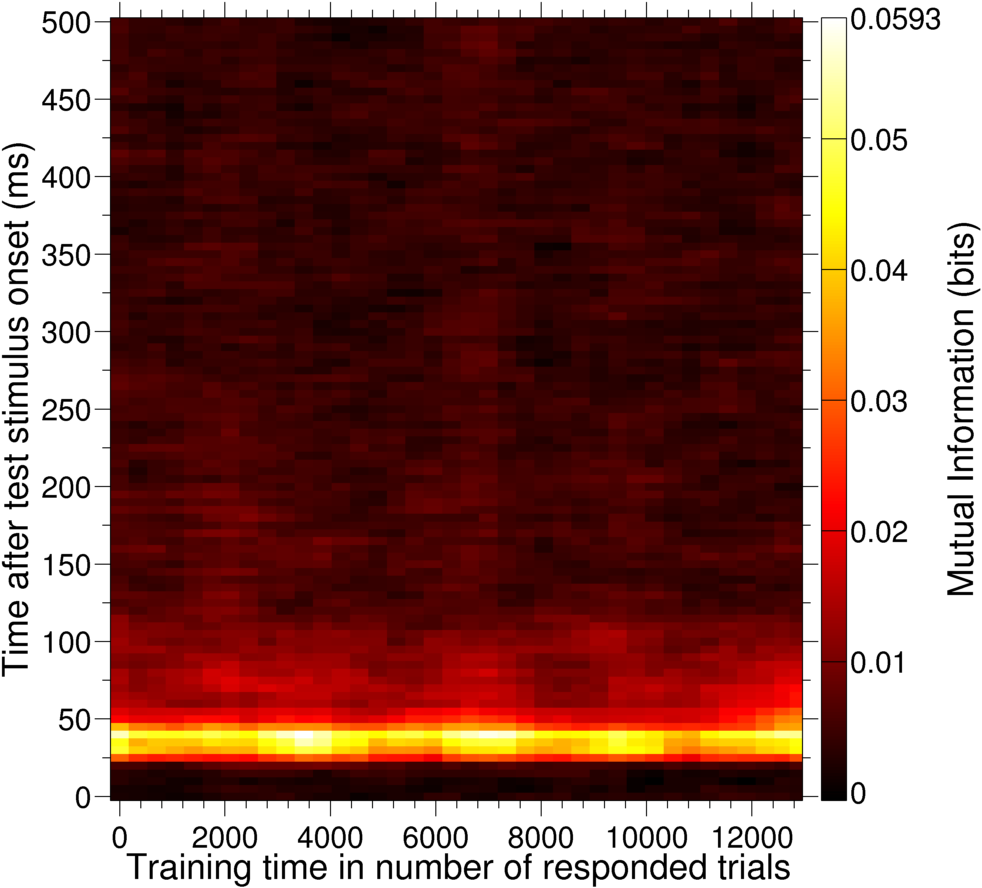
\includegraphics[scale=.25]{%
% figs/info/I_trialwise_blanco_v1_chmean23_s343-354,355.1,355.2,356-359_tp4_1bins_of_20ms_dr_pt_oc0_test_tc5-5-20,22-3-28,32,35-5-50,60,90_nt1400_ts350_rmvet1_rmvms0_pcolorhot_20120815T234452.png}
%         \caption{}
%         \label{fig:b1-1x20tp4ma}
%     \end{subfigure}
%     ~~
%     \begin{subfigure}[b]{0.5\linewidth}
%         \centering
%         \includegraphics[scale=.25]{%
% figs/info/I_trialwise_blanco_v1_chmean23_s343-354,355.1,355.2,356-359_tp1_1bins_of_20ms_dr_pt_oc0_test_tc5-5-20,22-3-28,32,35-5-50,60,90_nt1400_ts350_rmvet1_rmvms0_pcolorhot_20120815T234326.png}
%         \caption{}
%         \label{fig:b1-1x20tp1ma}
%     \end{subfigure}
%     \\
    \subfloat[][\label{fig:b1-1x20tp4}]{
        \centering
        \includegraphics[scale=.25]{%
figs/info/I_trialwise_blanco_v1_chmean23_s343-354,355.1,355.2,356-359_tp4_1bins_of_20ms_dr_pt_oc0_test_tc5-5-20,22-3-28,32,35-5-50,60,90_nt1400_ts350_rmvet1_rmvms1_pcolorhot_20120815T234741.png}
    }
    ~~
    \subfloat[][\label{fig:b1-1x20tp1}]{
        \centering
        \includegraphics[scale=.25]{%
figs/info/I_trialwise_blanco_v1_chmean23_s343-354,355.1,355.2,356-359_tp1_1bins_of_20ms_dr_pt_oc0_test_tc5-5-20,22-3-28,32,35-5-50,60,90_nt1400_ts350_rmvet1_rmvms1_pcolorbp_20120816T175451.png}
    }
    \\
    \subfloat[][\label{fig:b1-5x4tp4}]{
        \centering
        \includegraphics[scale=.25]{%
figs/info/I_trialwise_blanco_v1_chmean23_s343-354,355.1,355.2,356-359_tp4_5bins_of_4ms_dr_pt_oc0_test_tc5-5-20,22-3-28,32,35-5-50,60,90_nt1400_ts350_rmvet1_rmvms1_pcolorhot_20120815T234513.png}
    }
    ~~
    \subfloat[][\label{fig:b1-5x4tp1}]{
        \centering
        \includegraphics[scale=.25]{%
figs/info/I_trialwise_blanco_v1_chmean23_s343-354,355.1,355.2,356-359_tp1_5bins_of_4ms_dr_pt_oc0_test_tc5-5-20,22-3-28,32,35-5-50,60,90_nt1400_ts350_rmvet1_rmvms1_pcolorbp_20120816T175423.png}
    }
    \caption{\ac{M1} \ac{V1}: Mutual information between the test stimulus and \SI{20}{ms} of spiking activity, averaged across 23 channels.
The \ac{PT} bias correction method was used in all estimates of the information, and the modification to the spiking data to remove the artifact as described in \autoref{sec:ma} was performed.
The neural code used in \protect\subref{fig:b1-1x20tp4}, \protect\subref{fig:b1-1x20tp1} is a spike count code, whilst in \protect\subref{fig:b1-5x4tp4} and \protect\subref{fig:b1-5x4tp1} it is a spike timing code where the \SI{20}{ms} window was subdivided into 5 bins each of \SI{4}{ms}.
In \protect\subref{fig:b1-1x20tp4} and \protect\subref{fig:b1-5x4tp4} the spike-train is taken from the test presentation part of the trial;
for \protect\subref{fig:b1-1x20tp1} and \protect\subref{fig:b1-5x4tp1} the spike-train is taken from spontaneous pre-stimulus activity.
The data is sampled in intervals of \SI{350}{trials} in the $x$-direction and \SI{5}{ms} in the $y$-direction, so there is significant correlation between any pair of pixels in the image with less than 4 pixels between them in either cartesian direction.
% In \protect\subref{fig:b1-1x20tp4ma}, \protect\subref{fig:b1-1x20tp4}, and \protect\subref{fig:b1-5x4tp4}, the spike-train is taken from the test presentation part of the trial;
% for \protect\subref{fig:b1-1x20tp1ma}, \protect\subref{fig:b1-1x20tp1}, and \protect\subref{fig:b1-5x4tp1}, the spike-train is taken from spontaneous pre-stimulus activity.
% In \protect\subref{fig:b1-1x20tp4ma} and \protect\subref{fig:b1-1x20tp1ma} no attempt was made to remove the monitor artifact from the raw data, whilst in the rest of the panels the data was modified to counter this as described in \autoref{sec:ma}.
}
    \label{fig:b1-trialwise}
\end{figure}


% figs/info/I_trialwise_jack_v1_chmean25_s51-72_tp4_1bins_of_20ms_dr_pt_oc0_test_tc5-5-20,22-3-28,32,35-5-50,60,90_nt1400_ts350_rmvet1_rmvms0_pcolorhot_20120815T234410.png
% figs/info/I_trialwise_jack_v1_chmean25_s51-72_tp1_1bins_of_20ms_dr_pt_oc0_test_tc5-5-20,22-3-28,32,35-5-50,60,90_nt1400_ts350_rmvet1_rmvms0_pcolorhot_20120815T234245.png
% figs/info/I_trialwise_jack_v1_chmean25_s51-72_tp4_1bins_of_20ms_dr_pt_oc0_test_tc5-5-20,22-3-28,32,35-5-50,60,90_nt1400_ts350_rmvet1_rmvms1_pcolorhot_20120815T234701.png
% figs/info/I_trialwise_jack_v1_chmean25_s51-72_tp1_1bins_of_20ms_dr_pt_oc0_test_tc5-5-20,22-3-28,32,35-5-50,60,90_nt1400_ts350_rmvet1_rmvms1_pcolorbp_20120816T175411.png
% figs/info/I_trialwise_jack_v1_chmean25_s51-72_tp4_5bins_of_4ms_dr_pt_oc0_test_tc5-5-20,22-3-28,32,35-5-50,60,90_nt1400_ts350_rmvet1_rmvms1_pcolorhot_20120815T234434.png
% figs/info/I_trialwise_jack_v1_chmean25_s51-72_tp1_5bins_of_4ms_dr_pt_oc0_test_tc5-5-20,22-3-28,32,35-5-50,60,90_nt1400_ts350_rmvet1_rmvms1_pcolorbp_20120816T175343.png

\begin{figure}[htbp]
%     \begin{subfigure}[b]{0.5\linewidth}
%         \centering
%         \includegraphics[scale=.25]{%
% figs/info/I_trialwise_jack_v1_chmean25_s51-72_tp4_1bins_of_20ms_dr_pt_oc0_test_tc5-5-20,22-3-28,32,35-5-50,60,90_nt1400_ts350_rmvet1_rmvms0_pcolorhot_20120815T234410.png}
%         \caption{}
%         \label{fig:j1-1x20tp4ma}
%     \end{subfigure}
%     ~~
%     \begin{subfigure}[b]{0.5\linewidth}
%         \centering
%         \includegraphics[scale=.25]{%
% figs/info/I_trialwise_jack_v1_chmean25_s51-72_tp1_1bins_of_20ms_dr_pt_oc0_test_tc5-5-20,22-3-28,32,35-5-50,60,90_nt1400_ts350_rmvet1_rmvms0_pcolorhot_20120815T234245.png}
%         \caption{}
%         \label{fig:j1-1x20tp1ma}
%     \end{subfigure}
%     \\
    \subfloat[][\label{fig:j1-1x20tp4}]{
        \centering
        \includegraphics[scale=.25]{%
figs/info/I_trialwise_jack_v1_chmean25_s51-72_tp4_1bins_of_20ms_dr_pt_oc0_test_tc5-5-20,22-3-28,32,35-5-50,60,90_nt1400_ts350_rmvet1_rmvms1_pcolorhot_20120815T234701.png}
    }
    ~~
    \subfloat[][\label{fig:j1-1x20tp1}]{
        \centering
        \includegraphics[scale=.25]{%
figs/info/I_trialwise_jack_v1_chmean25_s51-72_tp1_1bins_of_20ms_dr_pt_oc0_test_tc5-5-20,22-3-28,32,35-5-50,60,90_nt1400_ts350_rmvet1_rmvms1_pcolorbp_20120816T175411.png}
    }
    \\
    \subfloat[][\label{fig:j1-5x4tp4}]{
        \centering
        \includegraphics[scale=.25]{%
figs/info/I_trialwise_jack_v1_chmean25_s51-72_tp4_5bins_of_4ms_dr_pt_oc0_test_tc5-5-20,22-3-28,32,35-5-50,60,90_nt1400_ts350_rmvet1_rmvms1_pcolorhot_20120815T234434.png}
    }
    ~~
    \subfloat[][\label{fig:j1-5x4tp1}]{
        \centering
        \includegraphics[scale=.25]{%
figs/info/I_trialwise_jack_v1_chmean25_s51-72_tp1_5bins_of_4ms_dr_pt_oc0_test_tc5-5-20,22-3-28,32,35-5-50,60,90_nt1400_ts350_rmvet1_rmvms1_pcolorbp_20120816T175343.png}
    }
    \caption{\ac{M2} \ac{V1}: Mutual information between the test stimulus and \SI{20}{ms} of spiking activity, averaged across 25 channels.
The \ac{PT} bias correction method was used in all estimates of the information.
Panels \protect\subref{fig:j1-1x20tp4}--\protect\subref{fig:j1-5x4tp1} are the same as for \autoref{fig:b1-trialwise}.
% The neural code used in \protect\subref{fig:j1-1x20tp4ma}--\protect\subref{fig:j1-1x20tp1} is a spike count code, whilst in \protect\subref{fig:j1-5x4tp4}, \protect\subref{fig:j1-5x4tp1} it is a spike timing code where the \SI{20}{ms} window was subdivided into 5 bins each of \SI{4}{ms}.
% In \protect\subref{fig:j1-1x20tp4ma}, \protect\subref{fig:j1-1x20tp4}, and \protect\subref{fig:j1-5x4tp4}, the spike-train is taken from the test presentation part of the trial;
% for \protect\subref{fig:j1-1x20tp1ma}, \protect\subref{fig:j1-1x20tp1}, and \protect\subref{fig:j1-5x4tp1}, the spike-train is taken from spontaneous pre-stimulus activity.
% In \protect\subref{fig:j1-1x20tp4ma} and \protect\subref{fig:j1-1x20tp1ma} no attempt was made to remove the monitor artifact from the raw data, whilst in the rest of the panels the data was modified to counter this as described in \autoref{sec:ma}.
}
    \label{fig:j1-trialwise}
\end{figure}

% figs/info/I_trialwise_blanco_v4_chmean31_s307,308,311,313,314,317,318,320,321,329-341_tp4_1bins_of_20ms_dr_pt_oc0_test_tc10-5-25,27-29,31-33,35,40-10-60_nt1400_ts350_rmvet1_rmvms0_pcolorhot_20120815T234508.png
% figs/info/I_trialwise_blanco_v4_chmean31_s307,308,311,313,314,317,318,320,321,329-341_tp1_1bins_of_20ms_dr_pt_oc0_test_tc10-5-25,27-29,31-33,35,40-10-60_nt1400_ts350_rmvet1_rmvms0_pcolorhot_20120815T234341.png
% figs/info/I_trialwise_blanco_v4_chmean31_s307,308,311,313,314,317,318,320,321,329-341_tp4_1bins_of_20ms_dr_pt_oc0_test_tc10-5-25,27-29,31-33,35,40-10-60_nt1400_ts350_rmvet1_rmvms1_pcolorhot_20120815T234756.png
% figs/info/I_trialwise_blanco_v4_chmean31_s307,308,311,313,314,317,318,320,321,329-341_tp1_1bins_of_20ms_dr_pt_oc0_test_tc10-5-25,27-29,31-33,35,40-10-60_nt1400_ts350_rmvet1_rmvms1_pcolorbp_20120816T175507.png
% figs/info/I_trialwise_blanco_v4_chmean31_s307,308,311,313,314,317,318,320,321,329-341_tp4_5bins_of_4ms_dr_pt_oc0_test_tc10-5-25,27-29,31-33,35,40-10-60_nt1400_ts350_rmvet1_rmvms1_pcolorhot_20120815T234528.png
% figs/info/I_trialwise_blanco_v4_chmean31_s307,308,311,313,314,317,318,320,321,329-341_tp1_5bins_of_4ms_dr_pt_oc0_test_tc10-5-25,27-29,31-33,35,40-10-60_nt1400_ts350_rmvet1_rmvms1_pcolorbp_20120816T175438.png


% % \begin{figure}[htbp]
% % %     \begin{subfigure}[b]{0.5\linewidth}
% % %         \centering
% % %         \includegraphics[scale=.25]{%
% % % figs/info/I_trialwise_blanco_v4_chmean31_s307,308,311,313,314,317,318,320,321,329-341_tp4_1bins_of_20ms_dr_pt_oc0_test_tc10-5-25,27-29,31-33,35,40-10-60_nt1400_ts350_rmvet1_rmvms0_pcolorhot_20120815T234508.png}
% % %         \caption{}
% % %         \label{fig:b4-1x20tp4ma}
% % %     \end{subfigure}
% % %     ~~
% % %     \begin{subfigure}[b]{0.5\linewidth}
% % %         \centering
% % %         \includegraphics[scale=.25]{%
% % % figs/info/I_trialwise_blanco_v4_chmean31_s307,308,311,313,314,317,318,320,321,329-341_tp1_1bins_of_20ms_dr_pt_oc0_test_tc10-5-25,27-29,31-33,35,40-10-60_nt1400_ts350_rmvet1_rmvms0_pcolorhot_20120815T234341.png}
% % %         \caption{}
% % %         \label{fig:b4-1x20tp1ma}
% % %     \end{subfigure}
% % %     \\
% %     \subfloat[][\label{fig:b4-1x20tp4}]{
% %         \centering
% %         \includegraphics[scale=.25]{%
% % figs/info/I_trialwise_blanco_v4_chmean31_s307,308,311,313,314,317,318,320,321,329-341_tp4_1bins_of_20ms_dr_pt_oc0_test_tc10-5-25,27-29,31-33,35,40-10-60_nt1400_ts350_rmvet1_rmvms1_pcolorhot_20120815T234756.png}
% %     }
% %     ~~
% %     \subfloat[][\label{fig:b4-1x20tp1}]{
% %         \centering
% %         \includegraphics[scale=.25]{%
% % figs/info/I_trialwise_blanco_v4_chmean31_s307,308,311,313,314,317,318,320,321,329-341_tp1_1bins_of_20ms_dr_pt_oc0_test_tc10-5-25,27-29,31-33,35,40-10-60_nt1400_ts350_rmvet1_rmvms1_pcolorbp_20120816T175507.png}
% %     }
% %     \\
% %     \subfloat[][\label{fig:b4-5x4tp4}]{
% %         \centering
% %         \includegraphics[scale=.25]{%
% % figs/info/I_trialwise_blanco_v4_chmean31_s307,308,311,313,314,317,318,320,321,329-341_tp4_5bins_of_4ms_dr_pt_oc0_test_tc10-5-25,27-29,31-33,35,40-10-60_nt1400_ts350_rmvet1_rmvms1_pcolorhot_20120815T234528.png}
% %     }
% %     ~~
% %     \subfloat[][\label{fig:b4-5x4tp1}]{
% %         \centering
% %         \includegraphics[scale=.25]{%
% % figs/info/I_trialwise_blanco_v4_chmean31_s307,308,311,313,314,317,318,320,321,329-341_tp1_5bins_of_4ms_dr_pt_oc0_test_tc10-5-25,27-29,31-33,35,40-10-60_nt1400_ts350_rmvet1_rmvms1_pcolorbp_20120816T175438.png}
% %     }
% %     \caption{\ac{M1} \ac{V4}: Mutual information between the test stimulus and \SI{20}{ms} of spiking activity, averaged across 30 channels.
% % The \ac{PT} bias correction method was used in all estimates of the information.
% % Panels \protect\subref{fig:b4-1x20tp4}--\protect\subref{fig:b4-5x4tp1} are the same as for \autoref{fig:b1-trialwise}.
% % % The neural code used in \protect\subref{fig:b4-1x20tp4ma}--\protect\subref{fig:b4-1x20tp1} is a spike count code, whilst in \protect\subref{fig:b4-5x4tp4}, \protect\subref{fig:b4-5x4tp1} it is a spike timing code where the \SI{20}{ms} window was subdivided into 5 bins each of \SI{4}{ms}.
% % % In \protect\subref{fig:b4-1x20tp4ma}, \protect\subref{fig:b4-1x20tp4}, and \protect\subref{fig:b4-5x4tp4}, the spike-train is taken from the test presentation part of the trial;
% % % for \protect\subref{fig:b4-1x20tp1ma}, \protect\subref{fig:b4-1x20tp1}, and \protect\subref{fig:b4-5x4tp1}, the spike-train is taken from spontaneous pre-stimulus activity.
% % % In \protect\subref{fig:b4-1x20tp4ma} and \protect\subref{fig:b4-1x20tp1ma} no attempt was made to remove the monitor artifact from the raw data, whilst in the rest of the panels the data was modified to counter this as described in \autoref{sec:ma}.
% % }
% %     \label{fig:b4-trialwise}
% % \end{figure}



% figs/info/I_trialwise_jack_v4_chmean20_s24-49_tp4_1bins_of_20ms_dr_pt_oc0_test_tc10-5-25,27-29,31-33,35,40-10-60_nt1400_ts350_rmvet1_rmvms0_pcolorhot_20120815T234433.png
% figs/info/I_trialwise_jack_v4_chmean20_s24-49_tp1_1bins_of_20ms_dr_pt_oc0_test_tc10-5-25,27-29,31-33,35,40-10-60_nt1400_ts350_rmvet1_rmvms1_pcolorbp_20120816T175433.png
% figs/info/I_trialwise_jack_v4_chmean20_s24-49_tp4_1bins_of_20ms_dr_pt_oc0_test_tc10-5-25,27-29,31-33,35,40-10-60_nt1400_ts350_rmvet1_rmvms1_pcolorhot_20120815T234723.png
% figs/info/I_trialwise_jack_v4_chmean20_s24-49_tp1_1bins_of_20ms_dr_pt_oc0_test_tc10-5-25,27-29,31-33,35,40-10-60_nt1400_ts350_rmvet1_rmvms1_pcolorhot_20120815T234559.png
% figs/info/I_trialwise_jack_v4_chmean20_s24-49_tp4_5bins_of_4ms_dr_pt_oc0_test_tc10-5-25,27-29,31-33,35,40-10-60_nt1400_ts350_rmvet1_rmvms1_pcolorhot_20120815T234455.png
% figs/info/I_trialwise_jack_v4_chmean20_s24-49_tp1_5bins_of_4ms_dr_pt_oc0_test_tc10-5-25,27-29,31-33,35,40-10-60_nt1400_ts350_rmvet1_rmvms1_pcolorbp_20120816T175404.png

\begin{figure}[htbp]
%     \begin{subfigure}[b]{0.5\linewidth}
%         \centering
%         \includegraphics[scale=.25]{%
% figs/info/I_trialwise_jack_v4_chmean20_s24-49_tp4_1bins_of_20ms_dr_pt_oc0_test_tc10-5-25,27-29,31-33,35,40-10-60_nt1400_ts350_rmvet1_rmvms0_pcolorhot_20120815T234433.png}
%         \caption{}
%         \label{fig:j4-1x20tp4ma}
%     \end{subfigure}
%     ~~
%     \begin{subfigure}[b]{0.5\linewidth}
%         \centering
%         \includegraphics[scale=.25]{%
% figs/info/I_trialwise_jack_v4_chmean20_s24-49_tp1_1bins_of_20ms_dr_pt_oc0_test_tc10-5-25,27-29,31-33,35,40-10-60_nt1400_ts350_rmvet1_rmvms0_pcolorhot_20120815T234307.png}
%         \caption{}
%         \label{fig:j4-1x20tp1ma}
%     \end{subfigure}
%     \\
    \subfloat[][\label{fig:j4-1x20tp4}]{
        \centering
        \includegraphics[scale=.25]{%
figs/info/I_trialwise_jack_v4_chmean20_s24-49_tp4_1bins_of_20ms_dr_pt_oc0_test_tc10-5-25,27-29,31-33,35,40-10-60_nt1400_ts350_rmvet1_rmvms1_pcolorhot_20120815T234723.png}
    }
    ~~
    \subfloat[][\label{fig:j4-1x20tp1}]{
        \centering
        \includegraphics[scale=.25]{%
figs/info/I_trialwise_jack_v4_chmean20_s24-49_tp1_1bins_of_20ms_dr_pt_oc0_test_tc10-5-25,27-29,31-33,35,40-10-60_nt1400_ts350_rmvet1_rmvms1_pcolorbp_20120816T175433.png}
    }
    \\
    \subfloat[][\label{fig:j4-5x4tp4}]{
        \centering
        \includegraphics[scale=.25]{%
figs/info/I_trialwise_jack_v4_chmean20_s24-49_tp4_5bins_of_4ms_dr_pt_oc0_test_tc10-5-25,27-29,31-33,35,40-10-60_nt1400_ts350_rmvet1_rmvms1_pcolorhot_20120815T234455.png}
    }
    ~~
    \subfloat[][\label{fig:j4-5x4tp1}]{
        \centering
        \includegraphics[scale=.25]{%
figs/info/I_trialwise_jack_v4_chmean20_s24-49_tp1_5bins_of_4ms_dr_pt_oc0_test_tc10-5-25,27-29,31-33,35,40-10-60_nt1400_ts350_rmvet1_rmvms1_pcolorbp_20120816T175404.png}
    }
    \caption{\ac{M2} \ac{V4}: Mutual information between the test stimulus and \SI{20}{ms} of spiking activity, averaged across 20 channels.
The \ac{PT} bias correction method was used in all estimates of the information.
Panels \protect\subref{fig:j4-1x20tp4}--\protect\subref{fig:j4-5x4tp1} are the same as for \autoref{fig:b1-trialwise}.
% The neural code used in \protect\subref{fig:j4-1x20tp4ma}--\protect\subref{fig:j4-1x20tp1} is a spike count code, whilst in \protect\subref{fig:j4-5x4tp4}, \protect\subref{fig:j4-5x4tp1} it is a spike timing code where the \SI{20}{ms} window was subdivided into 5 bins each of \SI{4}{ms}.
% In \protect\subref{fig:j4-1x20tp4ma}, \protect\subref{fig:j4-1x20tp4}, and \protect\subref{fig:j4-5x4tp4}, the spike-train is taken from the test presentation part of the trial;
% for \protect\subref{fig:j4-1x20tp1ma}, \protect\subref{fig:j4-1x20tp1}, and \protect\subref{fig:j4-5x4tp1}, the spike-train is taken from spontaneous pre-stimulus activity.
% In \protect\subref{fig:j4-1x20tp4ma} and \protect\subref{fig:j4-1x20tp1ma} no attempt was made to remove the monitor artifact from the raw data, whilst in the rest of the panels the data was modified to counter this as described in \autoref{sec:ma}.
}
    \label{fig:j4-trialwise}
\end{figure}

% 20, 30 and \SI{40}{ms} all tried.
% Mutual information increases as the duration increases as one would expect, but there is no other significant difference.
% Consequently only 20ms is shown in this section.

% More information with only correct trials used, but this could be due to differences in $P(S)$.

Turning our attention to the \ac{V4} results in \autoref{fig:b4-trialwise} and \autoref{fig:j4-trialwise}, we can see the effect of the transient is present in \ac{M1}'s data (at the later start time of \SI{75}{ms}), but not in \ac{M2}'s.
This is surprising because, looking at the rasters, in both animals there are some channels which exhibit a transient response and some which do not.

Similar to \ac{V1}, it seems as if there is four times as much information in the timebinned code compared with the count code.
However, there is much more information measured for the spontaneous activity data again.
This is not reduced by increasing the number of trials either.

For the spike count code in \ac{M2}, the spontaneous information is nearly distributed around 0, suggesting the bias has been all but removed and the data is of very high quality.
For this animal, we can see a distinct increase in the information content with time, for both the spike count and timing codes.
Simultaneously, there is a movement of the peak information to earlier times closer to the stimulus onset.

In \ac{M1}, there is a small increase in the information content with time which may or may not significant.
However, it is reassuring to see that this is not due to an improvement in the data with time, as the trend in the spontaneous activity information bias (\autoref{fig:j4-5x4tp1}) is a decrease with time.


%------------------------------------------------------------------------------
\subsection{Information in fine vs. coarse distinctions}

The difference between information about fine differences in contrast can be studied by only considering trials where the contrast presented is one of the middle 6 contrasts:
\SIlist{22;25;28;32;35;40}{\percent} for \ac{V1} and
\SIlist{27;28;29;31;32;33}{\percent} for \ac{V4}.
To keep the dimensionality of the stimulus the same, this has been compared to the information across some more separated contrasts:
\SIlist{5;15;22;40;50;90}{\percent} for \ac{V1} and
\SIlist{10;15;20;40;50;60}{\percent} for \ac{V4}.
For \ac{V4}, the group of coarsely differentiated contrasts is the outer most six contrasts, but for \ac{V1} the coarsely differentiated contrasts are alternate


\subsubsection{Results}

Comparing \autoref{fig:b1-1x20cc} and \autoref{fig:j1-1x20cc} where the outer 6 contrasts are included with \autoref{fig:b1-1x20tp4} and \autoref{fig:b1-1x20tp4} where all contrasts are included, it seems as if the amount of information has increased, which should not be possible.
However, the difference will be due to the difference in trials contained in each of the analyses.
In each case, an average of 100 trials per stimulus is used, but since the easier test conditions are presented less frequently, they are under-represented in \autoref{fig:b1-1x20tp4} and \autoref{fig:b1-1x20tp4} (about 75 trials per stimulus).
Obviously these are more discriminable, so the under-representation comparably reduces the information.

Looking at \ac{V1} (\autoref{fig:v1-fvc}), we observe there is much more information for \ac{M2} than \ac{M1}, as we found before.
The quality of the data seems to have severely hampered the analysis for \ac{M1}, destroying the the fine differences in the data needed to evaluate the information contained about fine contrast differences (\autoref{fig:b1-1x20fc}).

Unsurprisingly, there is more information when considering the coarsely distinct contrasts than the finer differences, as the neural activity is bound to be more discriminable for these.
For \ac{M2}, there is a small upward trend again for both coarse and fine contrast differences, which may or may not be genuine.

% figs/info/I_trialwise_blanco_v1_chmean23_s343-354,355.1,355.2,356-359_tp4_1bins_of_20ms_dr_pt_oc0_test_tc5,15,22,40,50,90_nt600_ts150_rmvet1_rmvms1_pcolorhot_20120816T011936.png
% figs/info/I_trialwise_blanco_v1_chmean23_s343-354,355.1,355.2,356-359_tp4_1bins_of_20ms_dr_pt_oc0_test_tc22-3-28,32,35,40_nt600_ts150_rmvet1_rmvms1_pcolorhot_20120816T011920.png
% figs/info/I_trialwise_jack_v1_chmean25_s51-72_tp4_1bins_of_20ms_dr_pt_oc0_test_tc5,15,22,40,50,90_nt600_ts150_rmvet1_rmvms1_pcolorhot_20120816T011822.png
% figs/info/I_trialwise_jack_v1_chmean25_s51-72_tp4_1bins_of_20ms_dr_pt_oc0_test_tc22-3-28,32,35,40_nt600_ts150_rmvet1_rmvms1_pcolorhot_20120816T011800.png

\begin{figure}[htbp]
    \subfloat[][\label{fig:b1-1x20cc}]{
        \centering
        \includegraphics[scale=.25]{%
figs/info/I_trialwise_blanco_v1_chmean23_s343-354,355.1,355.2,356-359_tp4_1bins_of_20ms_dr_pt_oc0_test_tc5,15,22,40,50,90_nt600_ts150_rmvet1_rmvms1_pcolorhot_20120816T011936.png}
    }
    ~~
    \subfloat[][\label{fig:j1-1x20cc}]{
        \centering
        \includegraphics[scale=.25]{%
figs/info/I_trialwise_jack_v1_chmean25_s51-72_tp4_1bins_of_20ms_dr_pt_oc0_test_tc5,15,22,40,50,90_nt600_ts150_rmvet1_rmvms1_pcolorhot_20120816T011822.png}
    }
    \\
    \subfloat[][\label{fig:b1-1x20fc}]{
        \centering
        \includegraphics[scale=.25]{%
figs/info/I_trialwise_blanco_v1_chmean23_s343-354,355.1,355.2,356-359_tp4_1bins_of_20ms_dr_pt_oc0_test_tc22-3-28,32,35,40_nt600_ts150_rmvet1_rmvms1_pcolorhot_20120816T011920.png}
    }
    ~~
    \subfloat[][\label{fig:j1-1x20fc}]{
        \centering
        \includegraphics[scale=.25]{%
figs/info/I_trialwise_jack_v1_chmean25_s51-72_tp4_1bins_of_20ms_dr_pt_oc0_test_tc22-3-28,32,35,40_nt600_ts150_rmvet1_rmvms1_pcolorhot_20120816T011800.png}
    }
    \caption{\ac{V1}: Fine vs. coarse contrast differences.
% Mutual information between the test stimulus and \SI{20}{ms} of spiking activity.
% The \ac{PT} bias correction method was used in all estimates of the information.
In the top panels, the six contrasts included are \{5, 15, 22, 40, 50, 90\}\%; bottom panels \{22, 25, 28, 32, 35, 40\}\%.
An average of 100 trials per stimulus is used in each of these.
Left panels are for \ac{M1}, right are \ac{M2}.
In each case, mutual information between the six test stimuli and \SI{20}{ms} of spiking activity was measured using a spike count code, and bias corrected using the \ac{PT} method.
% Panels \protect\subref{fig:b1-1x20cc} and \protect\subref{fig:b1-1x20fc} are for \ac{M1}, \protect\subref{fig:b1-1x20cc} and \protect\subref{fig:b1-1x20fc} for \ac{M2}.
}
    \label{fig:v1-fvc}
\end{figure}


% figs/info/I_trialwise_blanco_v4_chmean31_s307,308,311,313,314,317,318,320,321,329-341_tp4_1bins_of_20ms_dr_pt_oc0_test_tc10-5-20,40-10-60_nt600_ts150_rmvet1_rmvms1_pcolorhot_20120816T012120.png
% figs/info/I_trialwise_blanco_v4_chmean31_s307,308,311,313,314,317,318,320,321,329-341_tp4_1bins_of_20ms_dr_pt_oc0_test_tc27-29,31-33_nt600_ts150_rmvet1_rmvms1_pcolorhot_20120816T011952.png
% figs/info/I_trialwise_jack_v4_chmean20_s24-49_tp4_1bins_of_20ms_dr_pt_oc0_test_tc10-5-20,40-10-60_nt600_ts150_rmvet1_rmvms1_pcolorhot_20120816T011902.png
% figs/info/I_trialwise_jack_v4_chmean20_s24-49_tp4_1bins_of_20ms_dr_pt_oc0_test_tc27-29,31-33_nt600_ts150_rmvet1_rmvms1_pcolorhot_20120816T011843.png

\begin{figure}[htbp]
    \subfloat[][\label{fig:b4-1x20cc}]{
        \centering
        \includegraphics[scale=.25]{%
figs/info/I_trialwise_blanco_v4_chmean31_s307,308,311,313,314,317,318,320,321,329-341_tp4_1bins_of_20ms_dr_pt_oc0_test_tc10-5-20,40-10-60_nt600_ts150_rmvet1_rmvms1_pcolorhot_20120816T012120.png}
    }
    ~~
    \subfloat[][\label{fig:j4-1x20cc}]{
        \centering
        \includegraphics[scale=.25]{%
figs/info/I_trialwise_jack_v4_chmean20_s24-49_tp4_1bins_of_20ms_dr_pt_oc0_test_tc10-5-20,40-10-60_nt600_ts150_rmvet1_rmvms1_pcolorhot_20120816T011902.png}
    }
    \\
    \subfloat[][\label{fig:b4-1x20fc}]{
        \centering
        \includegraphics[scale=.25]{%
figs/info/I_trialwise_blanco_v4_chmean31_s307,308,311,313,314,317,318,320,321,329-341_tp4_1bins_of_20ms_dr_pt_oc0_test_tc27-29,31-33_nt600_ts150_rmvet1_rmvms1_pcolorhot_20120816T011952.png}
    }
    ~~
    \subfloat[][\label{fig:j4-1x20fc}]{
        \centering
        \includegraphics[scale=.25]{%
figs/info/I_trialwise_jack_v4_chmean20_s24-49_tp4_1bins_of_20ms_dr_pt_oc0_test_tc27-29,31-33_nt600_ts150_rmvet1_rmvms1_pcolorhot_20120816T011843.png}
    }
    \caption{\ac{V4}: Fine vs coarse contrast differences.
% Mutual information between the test stimulus and \SI{20}{ms} of spiking activity.
% The \ac{PT} bias correction method was used in all estimates of the information.
In the top panels, the six contrasts included are \{10, 15, 20, 40, 50, 60\}\%; bottom panels \{27, 28, 29, 31, 32, 33\}\%. An average of 100 trials per stimulus is used in each of these.
Left panels are for \ac{M1}, right are \ac{M2}.
In each case, mutual information between the six test stimuli and \SI{20}{ms} of spiking activity was measured using a spike count code, and bias corrected using the \ac{PT} method.
% Panels \protect\subref{fig:b1-1x20cc} and \protect\subref{fig:b1-1x20fc} are for \ac{M1}, \protect\subref{fig:b1-1x20cc} and \protect\subref{fig:b1-1x20fc} for \ac{M2}.
}
    \label{fig:v4-fvc}
\end{figure}

For \ac{V4}, we find there is no information about fine contrast differences in either animal (\autoref{fig:b4-1x20fc} and \autoref{fig:j4-1x20fc}).
The information about the coarse differences is higher than when all conditions are considered, for reasons discussed above, and these show the same trends as when we analysed all the conditions, in \autoref{fig:b4-1x20tp4} and \autoref{fig:j4-1x20tp4}.


\subsubsection{Discussion}

We did not find that learning was focused on the more difficult contrasts with the fine differences between them.
If there is an increase in the information in \ac{V1}, it is not very large and occurs for all groups of contrasts to the same degree.
Curiously, for \ac{V4}, it seems that the neurons improve their discriminability for the coarsely differentiated contrasts, but not the fine differences, which is the opposite to what was anticipated.
It could be that fine stimuli differences cannot be accurately resolved using the signals from only individual neurons, and concurrent signals from a population of neurons are needed for this to be finer discrimination to be possible.


%------------------------------------------------------------------------------
\subsection{Information in spike timing code vs. spike count code}

Because the possible responses in the spike timing and count codes have different dimensionality, they have different biases \citep{Panzeri2007} and it is not possible to compare them directly.
Consequently, to investigate how much more information there is in a spike timing based code we must consider a set of responses which have the same dimensionality, but lack the timing information.

To do this, the spike-timing response codes are taken, then shuffled across the 5 bins for every individual trial.%
\footnote{The shuffling of bins was performed using the open source Shuffle.m
available from \url{http://www.mathworks.com/matlabcentral/fileexchange/27076-shuffle}.}
Since the 5 bins are now in a random order, any information contained in their order is lost.
To make ensure the estimate of the information in the spike-timing code with the timing information destroyed was reasonable, the information was measured for five different shuffles%
% \footnote{The five shuffles were performed with a random seed linked to microsecond of execution time.}
 and then the mean was taken.

The information contained in the \SI{4}{ms} level spike timing can then be found by subtracting the mean shuffled information from the unshuffled information.


\subsubsection{Results}

For \ac{M2} \ac{V1}, there seems to be some information in the millisecond-level timing of the spikes during the transient response, but not afterward this has elapsed (\autoref{fig:v1-dif}, right-hand panels).
This band due to the transient is clearly well above the variance of the sampling for the rest of the window offsets.
However, the information in the transient is only present for the coarse contrasts and not for the fine contrasts.
For the fine contrast discrimination in \ac{M2} \ac{V1}, shown in \autoref{fig:j1-fdif}, (and possibly to a lesser degree on a couple of the other figures) there is an unusual effect where there seems to be more information in the shuffled bins than the unshuffled bins.\footnote{When this is analysed for the raw data with the artifact included, this is subtly more prominently on several of the plots.}

For \ac{M1} \ac{V1}, and also \ac{M1} \ac{V4}, there seems to be an increase in the information contained in the spike timing during the transient also.
However, these results are not as clear-cut as in \ac{M2} \ac{V1}.

% figs/info/I_diff_trialwise_dur=20ms_nshuf=1_blanco_v1_chmean23_s343-354,355.1,355.2,356-359_tp4_dr_pt_oc0_test_tc5-5-20,22-3-28,32,35-5-50,60,90_nt1400_ts350_rmvet1_rmvms1_pcolorbp_20120816T010538.png
% figs/info/I_diff_trialwise_dur=20ms_nshuf=1_blanco_v1_chmean23_s343-354,355.1,355.2,356-359_tp4_dr_pt_oc0_test_tc5,15,22,40,50,90_nt600_ts150_rmvet1_rmvms1_pcolorbp_20120816T004933.png
% figs/info/I_diff_trialwise_dur=20ms_nshuf=1_blanco_v1_chmean23_s343-354,355.1,355.2,356-359_tp4_dr_pt_oc0_test_tc22-3-28,32,35,40_nt600_ts150_rmvet1_rmvms1_pcolorbp_20120816T004908.png
% 
% figs/info/I_diff_trialwise_dur=20ms_nshuf=1_jack_v1_chmean25_s51-72_tp4_dr_pt_oc0_test_tc5-5-20,22-3-28,32,35-5-50,60,90_nt1400_ts350_rmvet1_rmvms1_pcolorbp_20120816T004517.png
% figs/info/I_diff_trialwise_dur=20ms_nshuf=1_jack_v1_chmean25_s51-72_tp4_dr_pt_oc0_test_tc5,15,22,40,50,90_nt600_ts150_rmvet1_rmvms1_pcolorbp_20120816T010526.png
% figs/info/I_diff_trialwise_dur=20ms_nshuf=1_jack_v1_chmean25_s51-72_tp4_dr_pt_oc0_test_tc22-3-28,32,35,40_nt600_ts150_rmvet1_rmvms1_pcolorbp_20120816T004555.png

\begin{figure}[htbp]
    \subfloat[][\label{fig:b1-alldif}]{
        \centering
        \includegraphics[scale=.25]{%
figs/info/I_diff_trialwise_dur=20ms_nshuf=1_blanco_v1_chmean23_s343-354,355.1,355.2,356-359_tp4_dr_pt_oc0_test_tc5-5-20,22-3-28,32,35-5-50,60,90_nt1400_ts350_rmvet1_rmvms1_pcolorbp_20120816T010538.png}
    }
    ~~
    \subfloat[][\label{fig:j1-alldif}]{
        \centering
        \includegraphics[scale=.25]{%
figs/info/I_diff_trialwise_dur=20ms_nshuf=1_jack_v1_chmean25_s51-72_tp4_dr_pt_oc0_test_tc5-5-20,22-3-28,32,35-5-50,60,90_nt1400_ts350_rmvet1_rmvms1_pcolorbp_20120816T004517.png}
    }
    \\
    \subfloat[][\label{fig:b1-cdif}]{
        \centering
        \includegraphics[scale=.25]{%
figs/info/I_diff_trialwise_dur=20ms_nshuf=1_blanco_v1_chmean23_s343-354,355.1,355.2,356-359_tp4_dr_pt_oc0_test_tc5,15,22,40,50,90_nt600_ts150_rmvet1_rmvms1_pcolorbp_20120816T004933.png}
    }
    ~~
    \subfloat[][\label{fig:j1-cdif}]{
        \centering
        \includegraphics[scale=.25]{%
figs/info/I_diff_trialwise_dur=20ms_nshuf=1_jack_v1_chmean25_s51-72_tp4_dr_pt_oc0_test_tc5,15,22,40,50,90_nt600_ts150_rmvet1_rmvms1_pcolorbp_20120816T010526.png}
    }
    \\
    \subfloat[][\label{fig:b1-fdif}]{
        \centering
        \includegraphics[scale=.25]{%
figs/info/I_diff_trialwise_dur=20ms_nshuf=1_blanco_v1_chmean23_s343-354,355.1,355.2,356-359_tp4_dr_pt_oc0_test_tc22-3-28,32,35,40_nt600_ts150_rmvet1_rmvms1_pcolorbp_20120816T004908.png}
    }
    ~~
    \subfloat[][\label{fig:j1-fdif}]{
        \centering
        \includegraphics[scale=.25]{%
figs/info/I_diff_trialwise_dur=20ms_nshuf=1_jack_v1_chmean25_s51-72_tp4_dr_pt_oc0_test_tc22-3-28,32,35,40_nt600_ts150_rmvet1_rmvms1_pcolorbp_20120816T004555.png}
    }
    \caption{\ac{V1}: Information in millisecond level spike timing.
% Mutual information between the test stimulus and \SI{20}{ms} of spiking activity.
% The \ac{PT} bias correction method was used in all estimates of the information.
The information with time-wise shuffled bins was subtracted from information in the spike time code with a \SI{20}{ms} window subdivided into 5 bins.
Information was bias corrected using the \ac{PT} method.
Left panels: \ac{M1}; Right: \ac{M2}.
Top panels: all contrasts, \{10, 15, 20, 25, 27, 28, 29, 31, 32, 33, 35, 40, 50, 60\}\%.
Centre panels: \{5, 15, 22, 40, 50, 90\}\%.
Bottom panels: \{22, 25, 28, 32, 35, 40\}\%.
An average of 100 trials per stimulus is used in the analysis for each.
% Panels \protect\subref{fig:b1-1x20cc} and \protect\subref{fig:b1-1x20fc} are for \ac{M1}, \protect\subref{fig:b1-1x20cc} and \protect\subref{fig:b1-1x20fc} for \ac{M2}.
}
    \label{fig:v1-dif}
\end{figure}


% figs/info/I_diff_trialwise_dur=20ms_nshuf=1_blanco_v4_chmean31_s307,308,311,313,314,317,318,320,321,329-341_tp4_dr_pt_oc0_test_tc10-5-20,40-10-60_nt600_ts150_rmvet1_rmvms1_pcolorbp_20120816T011506.png
% figs/info/I_diff_trialwise_dur=20ms_nshuf=1_blanco_v4_chmean31_s307,308,311,313,314,317,318,320,321,329-341_tp4_dr_pt_oc0_test_tc10-5-25,27-29,31-33,35,40-10-60_nt1400_ts350_rmvet1_rmvms1_pcolorbp_20120816T004958.png
% figs/info/I_diff_trialwise_dur=20ms_nshuf=1_blanco_v4_chmean31_s307,308,311,313,314,317,318,320,321,329-341_tp4_dr_pt_oc0_test_tc27-29,31-33_nt600_ts150_rmvet1_rmvms1_pcolorbp_20120816T005048.png
% 
% figs/info/I_diff_trialwise_dur=20ms_nshuf=1_jack_v4_chmean20_s24-49_tp4_dr_pt_oc0_test_tc10-5-20,40-10-60_nt600_ts150_rmvet1_rmvms1_pcolorbp_20120816T213446.png
% figs/info/I_diff_trialwise_dur=20ms_nshuf=1_jack_v4_chmean20_s24-49_tp4_dr_pt_oc0_test_tc10-5-25,27-29,31-33,35,40-10-60_nt1400_ts350_rmvet1_rmvms1_pcolorbp_20120816T004709.png
% figs/info/I_diff_trialwise_dur=20ms_nshuf=1_jack_v4_chmean20_s24-49_tp4_dr_pt_oc0_test_tc27-29,31-33_nt600_ts150_rmvet1_rmvms1_pcolorbp_20120816T004741.png

% % \begin{figure}[htbp]
% %     \subfloat[][\label{fig:b4-alldif}]{
% %         \centering
% %         \includegraphics[scale=.25]{%
% % figs/info/I_diff_trialwise_dur=20ms_nshuf=1_blanco_v4_chmean31_s307,308,311,313,314,317,318,320,321,329-341_tp4_dr_pt_oc0_test_tc10-5-25,27-29,31-33,35,40-10-60_nt1400_ts350_rmvet1_rmvms1_pcolorbp_20120816T004958.png}
% %     }
% %     ~~
% %     \subfloat[][\label{fig:j4-alldif}]{
% %         \centering
% %         \includegraphics[scale=.25]{%
% % figs/info/I_diff_trialwise_dur=20ms_nshuf=1_jack_v4_chmean20_s24-49_tp4_dr_pt_oc0_test_tc10-5-25,27-29,31-33,35,40-10-60_nt1400_ts350_rmvet1_rmvms1_pcolorbp_20120816T004709.png}
% %     }
% %     \\
% %     \subfloat[][\label{fig:b4-cdif}]{
% %         \centering
% %         \includegraphics[scale=.25]{%
% % figs/info/I_diff_trialwise_dur=20ms_nshuf=1_blanco_v4_chmean31_s307,308,311,313,314,317,318,320,321,329-341_tp4_dr_pt_oc0_test_tc10-5-20,40-10-60_nt600_ts150_rmvet1_rmvms1_pcolorbp_20120816T011506.png}
% %     }
% %     ~~
% %     \subfloat[][\label{fig:j4-cdif}]{
% %         \centering
% %         \includegraphics[scale=.25]{%
% % figs/info/I_diff_trialwise_dur=20ms_nshuf=1_jack_v4_chmean20_s24-49_tp4_dr_pt_oc0_test_tc10-5-20,40-10-60_nt600_ts150_rmvet1_rmvms1_pcolorbp_20120816T213446.png}
% %     }
% %     \\
% %     \subfloat[][\label{fig:b4-fdif}]{
% %         \centering
% %         \includegraphics[scale=.25]{%
% % figs/info/I_diff_trialwise_dur=20ms_nshuf=1_blanco_v4_chmean31_s307,308,311,313,314,317,318,320,321,329-341_tp4_dr_pt_oc0_test_tc27-29,31-33_nt600_ts150_rmvet1_rmvms1_pcolorbp_20120816T005048.png}
% %     }
% %     ~~
% %     \subfloat[][\label{fig:j4-fdif}]{
% %         \centering
% %         \includegraphics[scale=.25]{%
% % figs/info/I_diff_trialwise_dur=20ms_nshuf=1_jack_v4_chmean20_s24-49_tp4_dr_pt_oc0_test_tc27-29,31-33_nt600_ts150_rmvet1_rmvms1_pcolorbp_20120816T004741.png}
% %     }
% %     \caption{\ac{V4}: Information in millisecond level spike timing.
% % % Mutual information between the test stimulus and \SI{20}{ms} of spiking activity.
% % % The \ac{PT} bias correction method was used in all estimates of the information.
% % The information with time-wise shuffled bins was subtracted from information in the spike time code with a \SI{20}{ms} window subdivided into 5 bins.
% % Information was bias corrected using the \ac{PT} method.
% % Left panels: \ac{M1}; Right: \ac{M2}.
% % Top panels: all contrasts, \{5, 10, 15, 20, 22, 25, 28, 32, 35, 40, 45, 50, 60, 90\}\%.
% % Centre panels: \{10, 15, 20, 40, 50, 60\}\%.
% % Bottom panels: \{27, 28, 29, 31, 32, 33\}\%.
% % An average of 100 trials per stimulus is used in the analysis for each.
% % % Panels \protect\subref{fig:b1-1x20cc} and \protect\subref{fig:b1-1x20fc} are for \ac{M1}, \protect\subref{fig:b1-1x20cc} and \protect\subref{fig:b1-1x20fc} for \ac{M2}.
% % }
% %     \label{fig:v4-dif}
% % \end{figure}


For \ac{M2} \ac{V4}, there is no information in the spike timing measured on the millisecond timescale: not even during the transient response.

For any of these figures there certainly does not seem to be any change in the information contained in the spike timing alone, so it does not seem to be a trait which can be learned.

% This is true even if we only consider fine contrast differences as well, refuting our hypothesis that there will be more information in the spike timing for more finely differing stimuli contrasts.


\subsubsection{Discussion}

The observation about there being more information in the shuffled time-bins than when they are in their genuine order (\autoref{fig:j1-fdif}) should be an impossibility because shuffling the response bins around can only destroy information and cannot generate it as it is a random process, unrelated to the stimuli.
This could, however, be explained if spikes are similarly timed in the actual data for many stimuli, which causes their responses to be more similar than one would expect by chance.
In this case, there might be reliably more information measured in the shuffled bins due to the bias of the measurement being higher when the responses are less predictable.

The information in the precise spike timing for \ac{V1} would fit with previous results which have suggested there is information in the latency of the onset response
\citep{Reich2001,Tovee1993,Rolls2011}.
Moreover, \citep{Tovee1993,Rolls2011} indicates that for the primary visual cortex there is no information in the spike-timing beyond that of the spike code except for the limited amount of information given in the latency.
In addition, the work presented here suggests that although the latency of the response in \ac{V1} conveys information about the presented contrast, this is not a learned or learnable trait.


It was not found that there is more information contained in the spike timing for finer contrast differences.
This is contrary to the initial hypothesis, and contradicts several existing pieces of research \citep{Reich2001,Arabzadeh2006}, but it corroborates the items of research just mentioned indicating there is no information in spike-timing beyond the response latency \citep{Reich2001,Tovee1993,Rolls2011}.
As the bodies of work suggesting there would be differences for fine and coarse discrimination were based on recordings in the rat somatosensory system, whilst the latter is based in the visual cortex, this is not too surprising.
However, as we have already stated, any results from our analysis on spike timing codes are questionable due to the our control of the information in the spontaneous activity.


%------------------------------------------------------------------------------
\subsection{Spontaneous activity}

To check whether changes in the data quality between sessions and other differences between sessions could be influencing the results, the information theoretic analysis was also applied the spontaneous activity from the animal.
In particular, the spontaneous activity from prior to the sample presentation was used, so the animal had not yet seen the test contrast.
Although monkey's brain activity cannot possibly contain any genuine information about the test contrast, we expect to measure a non-zero value for the information content due to the sampling bias.

During the course of the analysis, results were inspected using \ac{PT} and using \ac{QE} for bias correction.
The plots were similar in distribution, and each gave a similar magnitude for the information.
However, \ac{PT} gave visibly lower variance than \ac{QE}, so only plots using \ac{PT} are presented in this results section.

Using the $\I_{\text{sh}}$ approach where the bias is corrected by shuffling bins across trials \citep{Montemurro2007} was also attempted for the spike timing code, but this increased the variance far too much to be of any practical use.
The unexpectedly significant increase in variance is probably due to the nature of the correlations between the bins which are being shuffled.

We also compared some of the results both with the monitor artifact left in the data and with the dataset redacted to have it removed.
There was no appreciable difference for any of the plots, though the amount of information went down when the data was redacted due to the loss of some of the spikes.


%==============================================================================
\section{Information at the population level}
\label{sec:dec-meth-lin}
%------------------------------------------------------------------------------

The input data to the decoding algorithm was chosen to be the total spike count during stimulus presentation from each trial.
This total is taken only for channels known to offer a consistent firing rate across sessions after the spontaneous activity matching process.
If there are 20 such channels in the dataset, taking the total number of spikes during stimulus presentation for each of the channels results in a 20-dimensional vector of population activity on each trial.

It should be noted that using all the spikes during the stimulus presentation period is likely to be sub-optimal, as not necessarily all of this period of time is carrying useful information about the stimuli.
The amount of spikes before the onset response, for instance, is clearly not stimulus dependent as it precedes the neural response to the stimulus, so it will only be a source of noise and  not useful for the decoding.
Furthermore, it is possible that the firing rate during the onset response might be more informative than the average firing rate across the whole presentation period.
However, finding the optimal window from which to take the spikes is an exercise in of itself.

The decoder used was a Fisher linear discriminant classifier.
Given a training dataset of labelled data points in 20D, the classifier will find the optimal 19D hyperplane such that it separates the two classes of points optimally, under the assumption that the two clusters to be separated are multivariate normal distributions.
The vector normal to the hyperplane is 
\begin{equation}
\vec{w} = \Sigma^{-1}\left(\vec{\mu_1}-\vec{\mu_0}\right)
\end{equation}
where $\Sigma$ is the covariance matrix between the two populations, as determined from the available labelled data, and $\vec{\mu_0}$ and $\vec{\mu_1}$ are the computed means of the two distributions.

Once a classifying hyperplane has been found, test data points can be classified by observing the side of the hyperplane on which they fall.
For a new data point, $\vec{x}$,  if
\begin{equation}
\vec{w}\cdot\vec{x}>c
\end{equation}
then we classify $\vec{x}$ as group 1 (higher than \SI{30}{\percent} contrast), otherwise we classify it as 0 (lower).

This was performed using the function \texttt{classify} with type `linear' in MATLAB.
For training and testing of the decoder, leave-one-out classification was used across each session individually.
This means that for a session of 500 trials, the decoder is trained on 499 trials with the spike counts for all the trials and the correct response (higher or lower than \SI{30}{\percent} contrast) and we then check whether the decoder identifies the remaining trial correctly.
This is repeated for all the 500 trials, and then the performance is defined as the proportion of trials which are identified correctly.
Training the decoder in this way means the decoding hyperplane used for classification is optimal for each individual session, but also different for each session.

The impact of noise correlations on the decoder is considered by comparing the regular decoder performance with the performance of a decoder applied to data which has been shuffled across trials under the same stimulus conditions.
After shuffling, specific neural response vectors no longer correspond to any particular trial, since the spike counts for each channel are taken from different trials.

%------------------------------------------------------------------------------
\subsection{Probabilistic Model}
\label{sec:dec-meth-prob}

As well as comparing the behavioural and decoding responses with the target responses to find a value for predictor performance, we can compare the behavioural and decoding responses with one another and find a value for their agreement, the proportion of trials on which the two responses are the same.

We would like to evaluate whether the behavioural responses are dependent on the firing rates of the recorded population of neurons.
This can be done by considering the behavioural and decoding response agreement, but in order to do this we need to construct a model of how much agreement we would expect to find if the two were completely independent, which will form our null hypothesis (NH) to compare against.

Throughout this work, it is assumed that the behavioural and decoding responses are given by a Bernoulli distribution.
In this model, there is a true probability, $p$, of the animal giving the correct answer to the task for each trial, which is sampled from on each of the trials.
When this is sampled over $n$ trials, we expect to find $np$ trials have been responded correctly and $n(1-p)$ incorrectly.

Hence the underlying true probability of a correct response can be approximated by taking the number of correct responses and dividing them by the total number of trials.
Using one of several statistical methods, we can find an estimate for a percentage confidence interval (PCI).
It is from this that error bars, indicated by the shaded regions surrounding line plots in \autoref{fig:dec_all_v1} and \autoref{fig:dec_all_v4}, are computed.
These are presented as the standard error, equivalent to a \SI{31.8}{\percent}  confidence interval within which \SI{68.2}{\percent} of data points are expected to lie.
(This has been done using the function \texttt{binofit} in MATLAB, which utilises the Clopper-Pearson method.
Although this is not the best method, it should be sufficient for our purposes.)

The behavioural performance is given by the estimated probability of the behavioural response being the same as the correct response, simply found by dividing the number of times the behavioural response matched the target response by the number of presentations.
The target response is of course whether or not the test stimulus is actually higher or lower than the sample.
Similarly, the decoding performance is the proportion of times the decoding response is the same as the target response; and the behavioural and decoding agreement is the proportion of times the behavioural and decoding responses are the same.

Using the estimated probabilities of the behavioural and decoding responses being correct, we can find an expected agreement between the behavioural and decoding responses if they are completely independent of one another, which constitutes the null hypothesis model (NH).
By comparing the observed agreement with the agreement we expect for independent variables, we can see whether or not behavioural responses are correlated with the decoded neural responses.

The theory behind the estimation of the agreement for independent binomial processes is described as follows.
Let us take two independent binomial variables, $X_1$ and $X_2$, which can either be in state $s_1$ with probabilities $p_1$ and $p_2$ respectively, or in state $s_2$ with probability $(1-p_1)$ and $(1-p_2)$.
If $X_1$ and $X_2$ are completely independent, we expect to find them in the same state with probability $p_1 \, p_2 + (1-p_1) (1-p_2)$.
Obviously, if $p_1$ and $p_2$ are both 0.5, there is a 0.5 chance of them being in the same state.
If $p_1$ and $p_2$ are both either higher or lower than 0.5, there is a higher chance of $X_1$ and $X_2$ being in the same state, and conversely if one is above and one below 0.5, there is a lower chance of them being in the same state.
This means that if the probabilities of the behavioural and decoding responses being correct rises during the perceptual learning process, we expect the proportion of trials on which they agree to rise as well, even if the two distributions are completely independent.

The initial model for the expected agreement between behaviour and decoding used a simple model as described above, where $p_1$ and $p_2$ are taken to be the overall probability of a correct response across all the test stimuli for behaviour and decoding respectively.
We will refer to this model as the single binomial model, as each predictor is modelled with a single binomial.
However, since there are 14 possible stimuli with varying difficulty, a more detailed model can be conceived in which the probability of a correct response for each predictor depends on the stimulus presented.
In this ``multi-binomial'' model, the set of conditions (different stimuli) is given by $C$, and each predictor, $i\in\{b,d\}$, can either be in the ``lower'' or ``higher'' state ($s_l$ or $s_h$).
For each $c\in C$, there is some probability $p_{il|c} := P(x_i=s_l|c)$ of predictor a being in the lower state.
Consequently, the probability of the two predictors being in the same state is given by
\begin{equation}
p_a = \sum_{c\in C} P(c) (p_{bl|c} \, p_{dl|c} + (1-p_{bl|c}) (1-p_{dl|c})
,\end{equation}
where $P(c)$ is the probability of condition $c$ being presented to the animal on any given trial.

We will assume that $c$ is a random variable, which is sampled from for each trial independent from prior trials.
This is a simplification of the actual condition selection process, ``delayed repetition''.
In this, the conditions for a set of trials are chosen in advance with $n$ appearances of each condition in a random order, after which any trial on which the animal responded incorrectly is repeated.
This means the single random variable approximation $P(c)$ is not uniform across the conditions, as harder conditions are presented more frequently.

For a given group of trials (such as, for instance, a single session), $P(c)$ can be estimated by dividing the number of times each appears by the total number of trials in the group.
Similarly, $p_{il|c}$ can be estimated by dividing the number of trials on which the predictor was in the lower state for a given condition by the number of trials where that condition was presented.

It is not immediately clear whether the single- or multi-binomial models will yield similar or different results.
Obviously, the multi-binomial model has more accurate detail and so should give a better result, but whether or not the single binomial should give a reasonable approximation is not obvious, though one would assume it would.
Applying the two models to the data and comparing them, we found the single binomial significantly underestimates the agreement which would really be found if the two predictors were completely independent.
Henceforth, only the more accurate multi-binomial model is considered.

The expected agreement under the assumption of two independent binomial processes gives us the null hypothesis model to compare against.
If the results of the analysis deviate significantly from this model, we can conclude the behavioural and neural decoded responses are correlated.
A $p<0.05$ significance boundary was found by sampling the NH model 100,000 times and noting the agreement for the fifth-percentile of samples.
During this sampling, the number of trials for each test condition was fixed with the same values as used in the experiment.
Since we are only interested in sessions where the behavioural and decoded responses agree more than they would if independent, a single-tailed test was used.
(NB: in the figures below, the single-tailed lower bound is also included for symmetry, so only \SI{90}{\percent} of the samples lie within the shaded region).

The multi-binomial model should not be confused with a multinomial distribution, which would map one random variable to $n$ possible responses.
The model used here is instead a two-step process where there are a set of binomial distributions, which binomial is used is determined by one random variable (the output of which is the same for both behaviour and decoder), and the output of the selected binomial is given by a second random variable.
In essence, the simple, single binomial model is similar to shuffling the responses across all trials regardless of condition, and the multi-binomial model we use is similar to shuffling the responses with the same condition presented.

%------------------------------------------------------------------------------
\subsection{Results}

\autoref{fig:dec_singles} shows how well the decoder does based only on data from individual channels.
The performance was measured as described in \autoref{sec:dec-meth-lin} for each session, and then averaged over all sessions.
[perhaps a histogram would show how these are distributed better?]

\autoref{fig:dec_nbest} indicates how the performance of the decoder improves as more channels are added.
We can see that the decoder performance saturates after around 10 channels are included in the training data, but at a perforance which is still far from the ideal.
After this, including additional channels yields only a slight increase in performance, suggesting nearly all the information contained in the remaining channels is redundant, as it has already been given in the first 10 channels.
[would be better to look at how the decoding perfarmance is distributed across all possible sets of $n$ channels, rather than just the best set of $n$ channels] [this should be compared with shuffled data to see what the impact is and whether performance does not saturate when correlations are removed as per some previous papers [cite]]

NB: the order in which channels were added in \autoref{fig:dec_nbest} is not the same ordering as they are shown in \autoref{fig:dec_singles}.

\begin{figure}[htbp]
    \subfloat[][\label{fig:dec_singles}]{
        \centering
        \includegraphics[width=0.47\linewidth]{%
figs/decoding/2FC_singles.eps}
    }
    ~~
    \subfloat[][\label{fig:dec_nbest}]{
        \centering
        \includegraphics[width=0.47\linewidth]{%
figs/decoding/2FC_nbest_all.eps}
    }
    \caption{
\protect\subref{fig:dec_singles}: Distribution of decoder performance based on spike rate for individual channels, sorted by performance.
\protect\subref{fig:dec_nbest}: Decoding performance versus number of channels included in spiking data.
Channels were added one at a time, chosen so they maximise the decoder performance for that number of channels whilst keeping all the channels which had come before.
}
    \label{fig:dec_n}
\end{figure}

For each of the datasets, the performance decreases as the last 3 channels are added (\autoref{fig:dec_nbest}).
I speculate that this is because these channels only contain redundant information, and the increase in dimensionality decreases the quality of the classifier selected from the finite training data available.


\begin{figure}[htbp]
    \subfloat[][\label{fig:dec_b4_allp}]{
        \centering
	\includegraphics[width=0.47\linewidth]{figs/decoding/perf_v4_blanco.eps}
    }
    ~~
    \subfloat[][\label{fig:dec_j4_allp}]{
        \centering
	\includegraphics[width=0.47\linewidth]{figs/decoding/perf_v4_jack.eps}
    }
    \caption{%
    Decoding analysis for \ac{V4}.
    Performance of behavioural and decoding predictors by session, averaged across all conditions.
    Left panels: \ac{M1}. Right: \ac{M2}.
	Along the x-axis, `Session' is the animal's unique session ID, which increments by one for every day of training.
    On the y-axis, `proportion correct' is the proportion of trials for which the response is the same as the target.
    This is presented for behavioural performance (black), decoder performance (blue), and decoder performance when trials are shuffled, destroying noise correlations (red; see text).
}
    \label{fig:dec_all_v4}
\end{figure}

\begin{figure}[htbp]
    \subfloat[][\label{fig:dec_b1_allp}]{
        \centering
	\includegraphics[width=0.47\linewidth]{figs/decoding/perf_v1_blanco.eps}
    }
    ~~
    \subfloat[][\label{fig:dec_j1_allp}]{
        \centering
	\includegraphics[width=0.47\linewidth]{figs/decoding/perf_v1_jack.eps}
    }
    \caption{%
    Decoding analysis for \ac{V1}.
    Performance of behavioural and decoding predictors by session, averaged across all conditions.
    Left panels: \ac{M1}. Right: \ac{M2}.
	Along the x-axis, `Session' is the animal's unique session ID, which increments by one for every day of training.
    On the y-axis, `proportion correct' is the proportion of trials for which the response is the same as the target.
    This is presented for behavioural performance (black), decoder performance (blue), and decoder performance when trials are shuffled, destroying noise correlations (red; see text).
}
    \label{fig:dec_all_v1}
\end{figure}



For \ac{M2} \ac{V4}, the trend in increase for behavioural performance is well matched by the change in performance of the decoder (\autoref{fig:dec_j4_allp}, blue and red lines).
In contrast to this, for \ac{M1} \ac{V4} we see the decoding performance is steady despite training, although it should be noted that the increase in behavioural performance was not so large for this animal.

For \ac{M2} \ac{V1}, there is a small gradual increase in decoder performance throughout training, though the increase does not match the timescales and rate of the increase in behavioural performance which is a much sharper transition.
Results for \ac{M2} \ac{V1} could be interpreted as indicating that no further improvements can be obtained from changes in \ac{V1}, and the behavioural performance is limited by the performance of the decoder.
For \ac{M1} \ac{V1}, there is a decrease in decoder in performance despite the increase in behavioural performance (\autoref{fig:dec_b1_allp}, blue and red lines respectively).


Shuffling the trials to destroy any noise correlations provides an improvement in performance for the data from \ac{M2}, indicating that noise correlations are detrimental to the successful decoding of stimuli.
However, there is no significant difference in decoder performance before and after shuffling for \ac{M1} datasets, which suggests noise correlations have no impact on decoding the contrast of stimuli using firing rate data from a population of neurons.
For \ac{M2} \ac{V1}, the benefit from shuffling seems to be reduced with training; the shuffled decoding performance is reasonably steady throughout training whilst the decoder with noise correlations included increases in performance, closing the gap.

% \marginnote{It might well be better to plot, for each area, the performances for both animals on the same plot and the expected vs observed behavioural agreement for both animals on a seperate plot.}


\begin{figure}[htbp]
    \subfloat[][\label{fig:decag_b4_allp}]{
        \centering
	\includegraphics[width=0.47\linewidth]{figs/decoding/agree_v4_blanco.eps}
    }
    ~~
    \subfloat[][\label{fig:decag_j4_allp}]{
        \centering
	\includegraphics[width=0.47\linewidth]{figs/decoding/agree_v4_jack.eps}
    }
    \caption{%
    Decoding analysis for \ac{V4}.
    Trial-to-trial agreement between behavioural and decoding predictors.
    Left panels: \ac{M1}. Right: \ac{M2}.
	Along the x-axis, `Session' is the animal's unique session ID, which increments by one for every day of training.
    On the y-axis is the proportion of trials for which the response is the same as the behavioural response.
    The agreement between behaviour and decoding (unshuffled only) is presented alongside the null hypothesis of completely independent binomial distributions.
    The dashed line indicates the 95\% confidence interval of the null hypothesis.
}
    \label{fig:decag_all_v4}
\end{figure}

\begin{figure}[htbp]
    \subfloat[][\label{fig:decag_b1_allp}]{
        \centering
	\includegraphics[width=0.47\linewidth]{figs/decoding/agree_v1_blanco.eps}
    }
    ~~
    \subfloat[][\label{fig:decag_j1_allp}]{
        \centering
	\includegraphics[width=0.47\linewidth]{figs/decoding/agree_v1_jack.eps}
    }
    \caption{%
    Decoding analysis for \ac{V1}.
    Trial-to-trial agreement between behavioural and decoding predictors.
    Left panels: \ac{M1}. Right: \ac{M2}.
	Along the x-axis, `Session' is the animal's unique session ID, which increments by one for every day of training.
    On the y-axis is the proportion of trials for which the response is the same as the behavioural response.
    The agreement between behaviour and decoding (unshuffled only) is presented alongside the null hypothesis of completely independent binomial distributions.
    The dashed line indicates the 95\% confidence interval of the null hypothesis.
}
    \label{fig:decag_all_v1}
\end{figure}


With regards to the behavioural and decoding response agreement, we find there is no consistent significant deviation from the null hypothesis for \ac{V1} data.
There are a couple of sessions where unshuffled agreement is above the boundary for significance for each of the animals, but this is not a consistent effect.
The agreement between shuffled decoding and behaviour does not deviate from the corresponding null hypothesis.
This shows that the shuffled is higher than the unshuffled decoding agreement only because the shuffled decoder is more accurate at matching the target response.

For \ac{V4}, we see that the agreement does not deviate significantly from the null hypothesis for earlier sessions, but after a cut off point all later sessions do (\ac{M1}: all sessions before 321 are not, after 329 are significant; \ac{M2}: Before 28 are not, after 28 are significant).
The effect is stronger for \ac{M2}, but present for both animals.
This indicates that the behavioural responses and the decoded responses based on the neural data were not notably correlated, but have become so with training.

Because the shuffled decoded responses are more accurate (with respect to the target response), they are predicted under the null hypothesis to be in better agreement with the behavioural responses.
However we observe these are in worse agreement than the unshuffled decoding, and do not deviate from the corresponding NH line.

A more detailed breakdown of these results with subsets of the 14 conditions is given in \autoref{fig:dec_detail_b1} and \autoref{fig:dec_detail_j4}.
Comparing \autoref{fig:dec_b4_6easy_a} and \autoref{fig:dec_j4_6easy_a} with \autoref{fig:dec_b4_6hard_a} and \autoref{fig:dec_j4_6hard_a}, we can see that the decoding responses for the easier conditions fit the null hypothesis model, whilst the more challenging conditions do not and have a statistically significant agreement with the animal behaviour.
